\documentclass[twoside,numbers,spanish]{clases}

\usepackage{multirow}
\usepackage{float}

\author{Jeremias Vozzi}
\title{Biosensor electroqu\'imico en sustrato flexible mediante electr\'onica impresa funcional}
\degree{Ingeniero Electr\'onico}
\supervisor{\begin{tabular}{c @{\hspace{1,6cm}} c @{\hspace{1,6cm}} c}
Dra. Ing. Liliana Fraigi & Ing. Mijal Mass & DI. Mariano Roberti\\
lilifraigi$@$gmail.com & mmass$@$gmail.com & roberti.mariano$@$gmail.com\\
\end{tabular}
\begin{tabular}{c}
Centro de Micro y Nanoelectr\'onica del Bicentenario\\
Instituto Nacional de Tecnolog\'ia Industrial\\
San Martín, Buenos Aires, Argentina\\
\end{tabular}
}
\institution{Universidad Nacional de San Mart\'in}
\faculty{Escuela de Ciencia y Tecnolog\'ia}

\geometry{top=20mm,bottom=40mm,inner=40mm,outer=25mm}

\hyperlinking

\begin{document}

%% ## Construye tu propia portada ##
%% 
%% Una portada se conforma por una secuencia de "Blocks" que incluyen
%% piezas individuales de informaci'on. Un "Block" puede incluir, por
%% ejemplo, el t'itulo del documento, una im'agen (logotipo de la universidad),
%% el nombre del autor, nombre del supervisor, u cualquier otra pieza de
%% informaci'on.
%%
%% Cada "Block" aparece centrado horizontalmente en la p'agina y,
%% verticalmente, todos los "Blocks" se distruyen de manera uniforme 
%% a lo largo de p'agina.
%%
%% Nota tambi'en que, dentro de un mismo "Block" se pueden cortar
%% lineas usando el comando \\
%%
%% El tama'no del texto dentro de un "Block" se puede modificar usando uno de
%% los comandos:
%%   \small      \LARGE
%%   \large      \huge
%%   \Large      \Huge
%%
%% Y el tipo de letra se puede modificar usando:
%%   \bfseries - negritas
%%   \itshape  - it'alicas
%%   \scshape  - small caps
%%   \slshape  - slanted
%%   \sffamily - sans serif


\begin{titlepage}
  \TitleBlock[\bigskip]{\scshape\insertinstitution}
  \TitleBlock[\bigskip]{\scshape\insertfaculty}
  \TitleBlock[\bigskip]{
\includegraphics[height=4cm]{Figuras/logo_unsam}}
  \TitleBlock[\bigskip]{\bfseries\Large\scshape\inserttitle}
  \TitleBlock[\bigskip]{\scshape\large
  Proyecto final integrador para obtener el grado de \insertdegree}
  \TitleBlock{\bfseries\scshape Autor}  
  \TitleBlock[\vspace*{0,1cm}]{\scshape\insertauthor}
  \TitleBlock{jeremias.vozzi$@$gmail.com}  
  \TitleBlock[\bigskip]{\bfseries\scshape Tutores}
  \TitleBlock{\small\insertsupervisor}
  \TitleBlock[\vspace*{1cm}]{\bfseries\large\insertsubmitdate}
\end{titlepage}


%% Nota 2:
%% Normalmente, el espacio entre "Blocks" se extiende de modo que el
%% contenido se reparte uniformemente sobre toda la p'agina. Este
%% comportamiento se puede modificar para mantener fijo, por ejemplo, el
%% espacio entre un par de "Blocks". Escribiendo:
%%   \TitleBlock{Bloque 1}
%%   \TitleBlock[\bigskip]{Bloque2}
%% se deja un espacio "grande" y de tama~no fijo entre el bloque 1 y 2.
%% Adem'as de \bigskip est'an tambi'en \smallskip y \medskip. Si necesitas
%% aun m'as control puedes usar tambi'en, por ejemplo, \vspace*{2cm}[\vspace*{0,5cm}].




\begin{center}
\vspace*{8cm}

El presente trabajo fue escrito en \LaTeX{}. Los gráficos se realizaron con GNUPlot y los esquemas fueron dibujados con InkScape.


\end{center}

\prefacesection{Agradecimientos}

Como última página que escribo de este documento quisiera finalizar agradeciendo a todos los que aportaron desde mis comienzos como estudiante hasta la culminación de mi carrera de grado mediante este proyecto.

En especial:

A Lili, Mijal y Mariano, tutores de este proyecto. Lograron interesarme en el proyecto desde la primera reunión. Siempre motivados y dispuestos a ayudarme en lo que hiciera falta para avanzar. Me dieron la libertad para llevar adelante los trabajos, las herramientas, me brindaron sus conocimientos y el apoyo para obtener los mejores resultados posibles.

Al grupo de excelentes profesionales que integran el Centro de Micro y Nanoelectrónica del Bicentenario. Me recibieron desde el primer día como uno más y siempre atentos a ayudarme en lo que necesitaba.

A Gustavo Giménez por su enorme ayuda con la caracterización, su clase magistral de electroquímica y sus recomendaciones para el proyecto.

Al Instituto Nacional de Tecnología Industrial por brindarme los materiales, el espacio y la ayuda de sus integrantes para poder llevar a cabo el trabajo.

A la Universidad Nacional de San Martín, por brindar excelente educación pública y gratuita.

Al Ing. Sinderman, Director de la Carrera, por tener su oficina siempre abierta, dispuesto a escuchar y ayudar a los alumnos para que puedan lograr sus objetivos. Además, por dar las mejores clases de Teoría de Circuitos que un estudiante de electrónica pueda pedir.

Al Ing. Polenta por dar las mejores y más interesantes clases (también las más difíciles) de la carrera.

A los amigos que fui haciendo a lo largo de estos años, especialmente a Gastón, Alan y Mauri con los que nos impulsamos mutuamente en los últimos grandes esfuerzos de finales y trabajos prácticos.

A mis amigos Lucas, Agustin, Andi, Fede, Dexter y Stefan. Compañeros de toda la vida.

A mis tíos y primos por apoyarme y bancarme en los momentos que más lo necesité.

A mis abuelos, que ya no están pero me inspiraron siempre a luchar y esforzarse para conseguir lo que uno se proponga.

A mi mamá Graciela y mi papá Carlos que me apoyaron en todas mis decisiones, me dieron todo y más de lo que necesité. 

Por último dedicarlo especialmente a Lucila, que me banca siempre, me brinda su alegría y su cariño día a día.
\prefacesection{Anteproyecto}
Previo al desarrollo del proyecto se describe el planeamiento que se realizó, siguiendo los lineamientos del Project Management.
\\
\begin{flushleft}
{\Large \textbf{Project charter}}
\end{flushleft}
\begin{figure}[H]
  \centering
    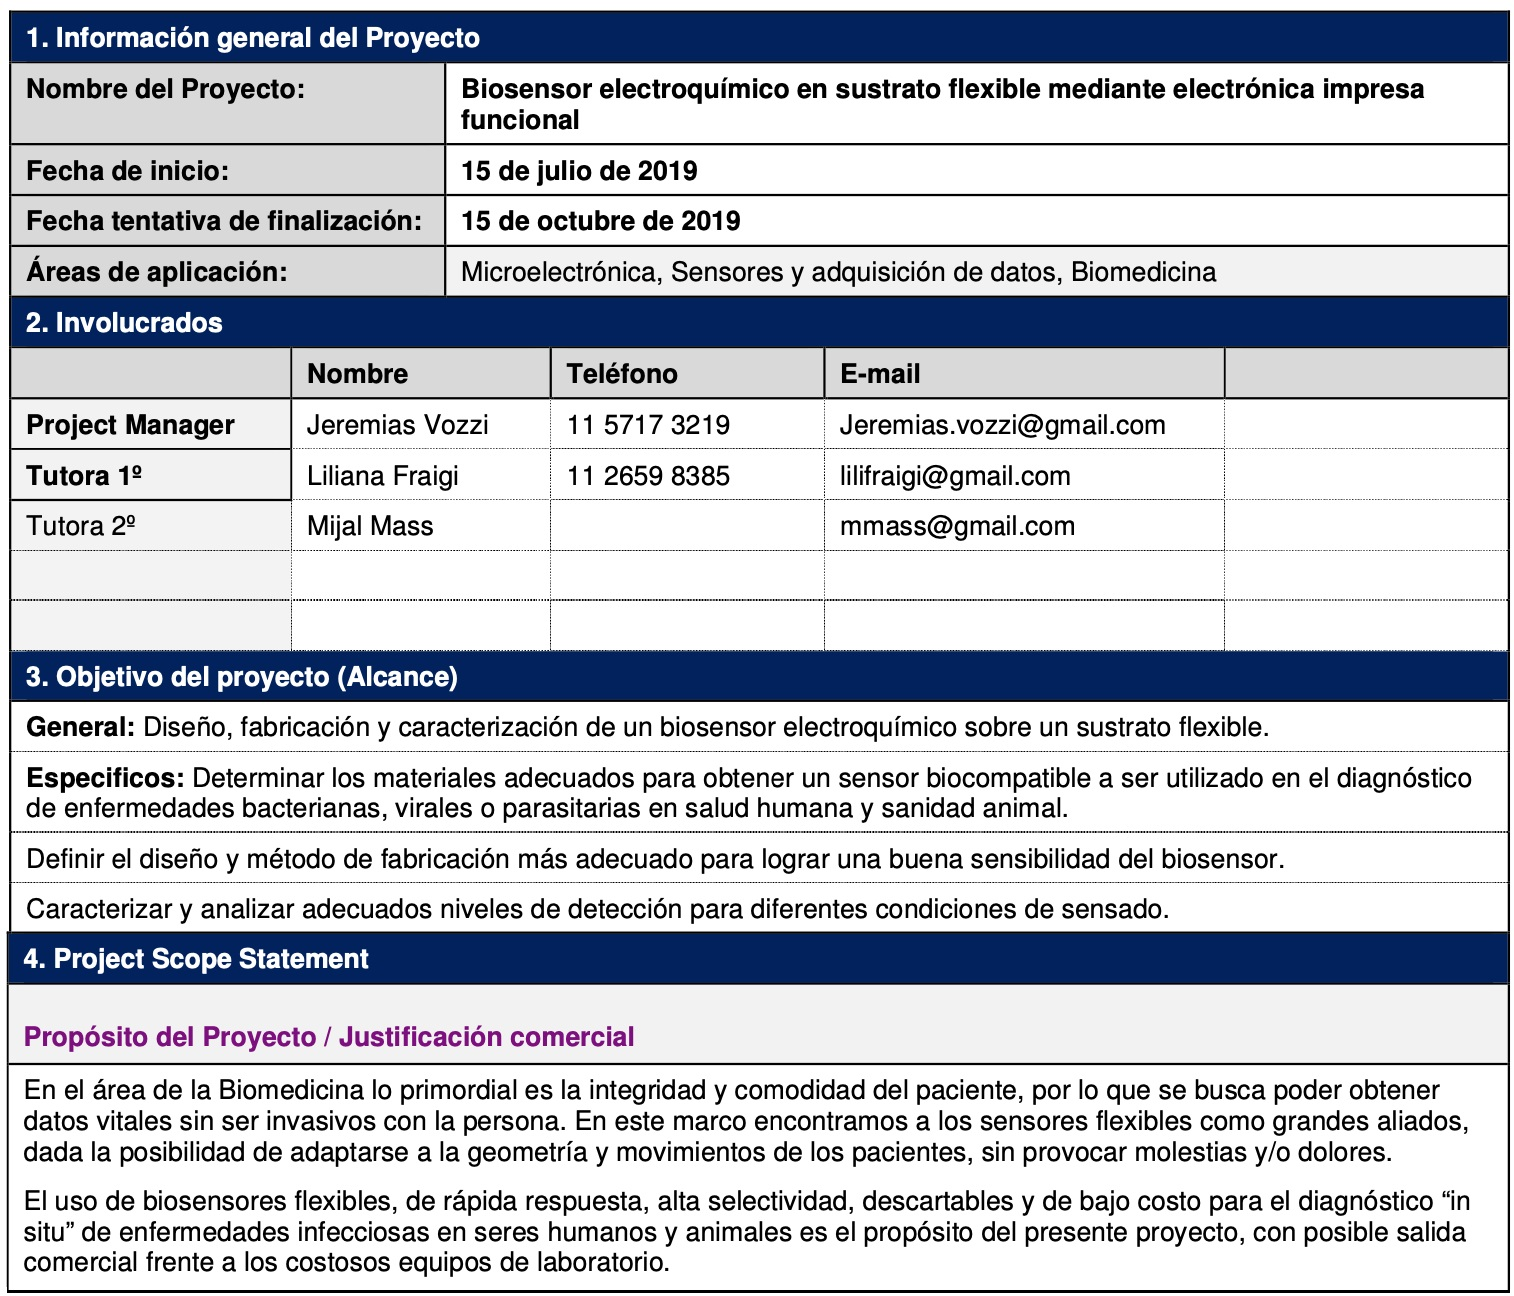
\includegraphics[width=1\textwidth]{Figuras/ProjChart1}
  \label{fig:ProjChart1}
\end{figure}
\begin{figure}[H]
  \centering
    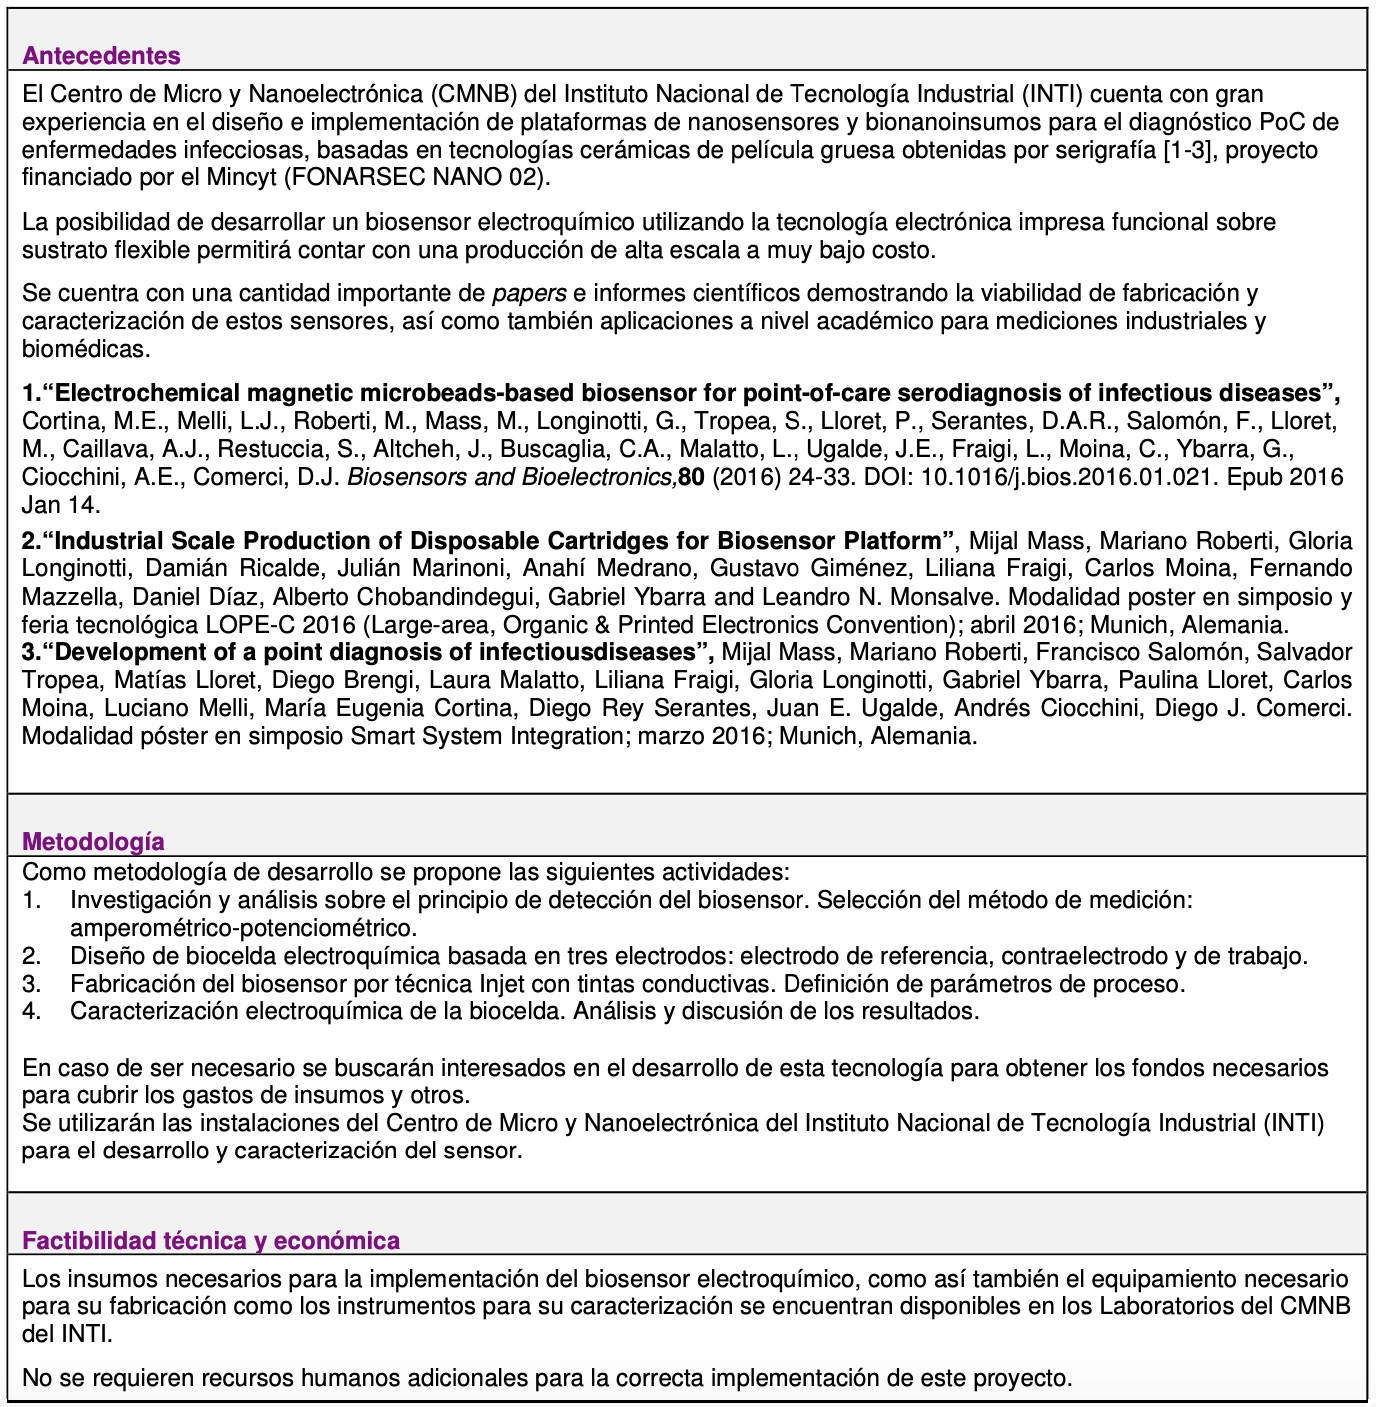
\includegraphics[width=1\textwidth]{Figuras/ProjChart2}
  \label{fig:ProjChart2}
\end{figure}
\begin{figure}[H]
  \centering
    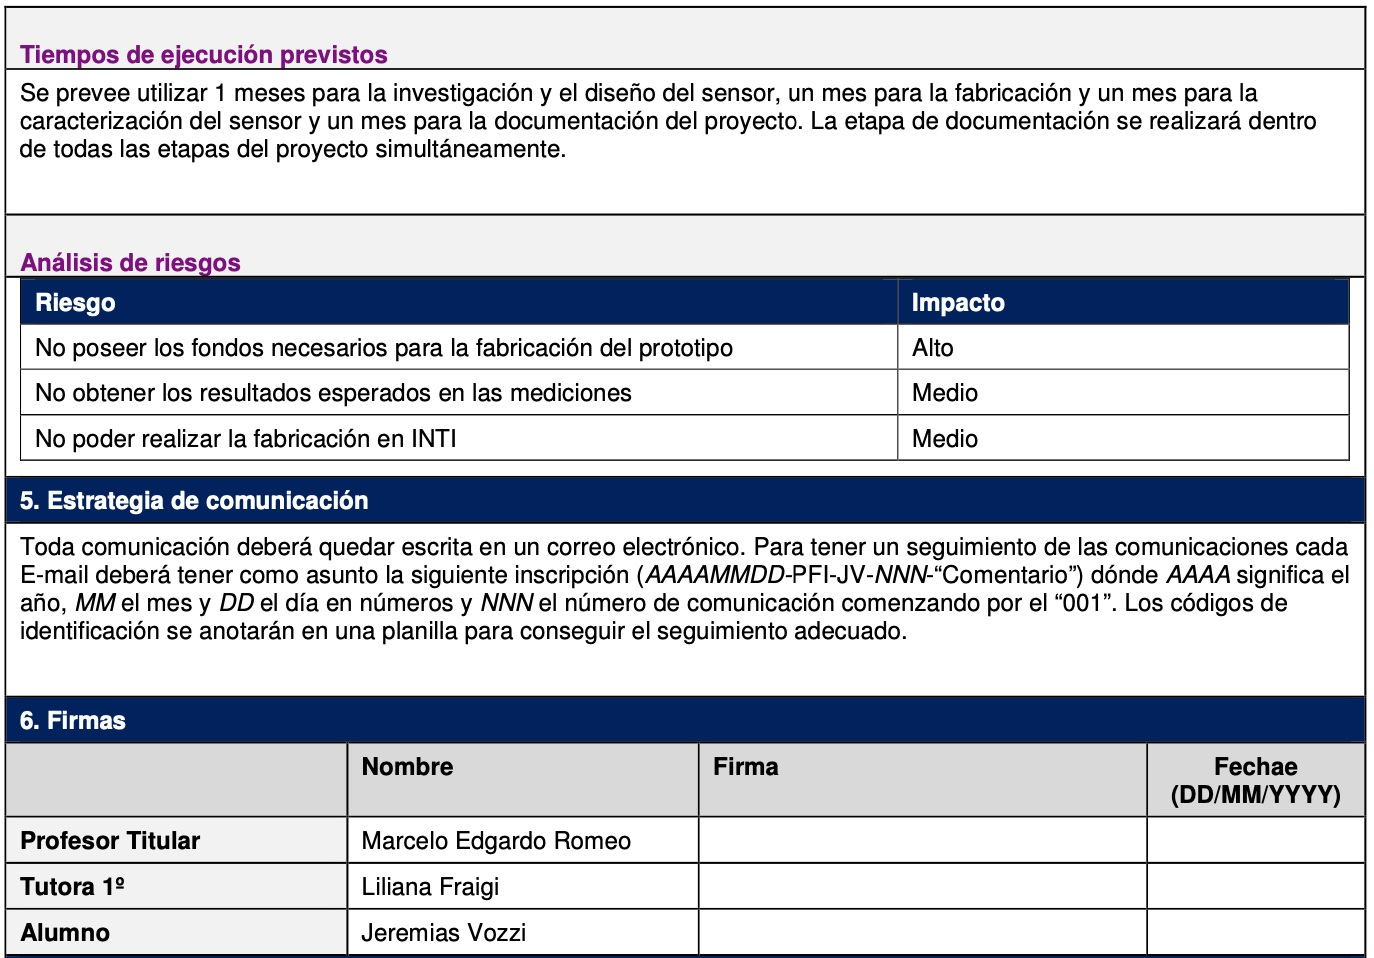
\includegraphics[width=1\textwidth]{Figuras/ProjChart3}
  \label{fig:ProjChart3}
\end{figure}
\newpage 
\begin{flushleft}
{\Large \textbf{Work breakdown structure}}
\end{flushleft}
\begin{figure}[H]
  \centering
    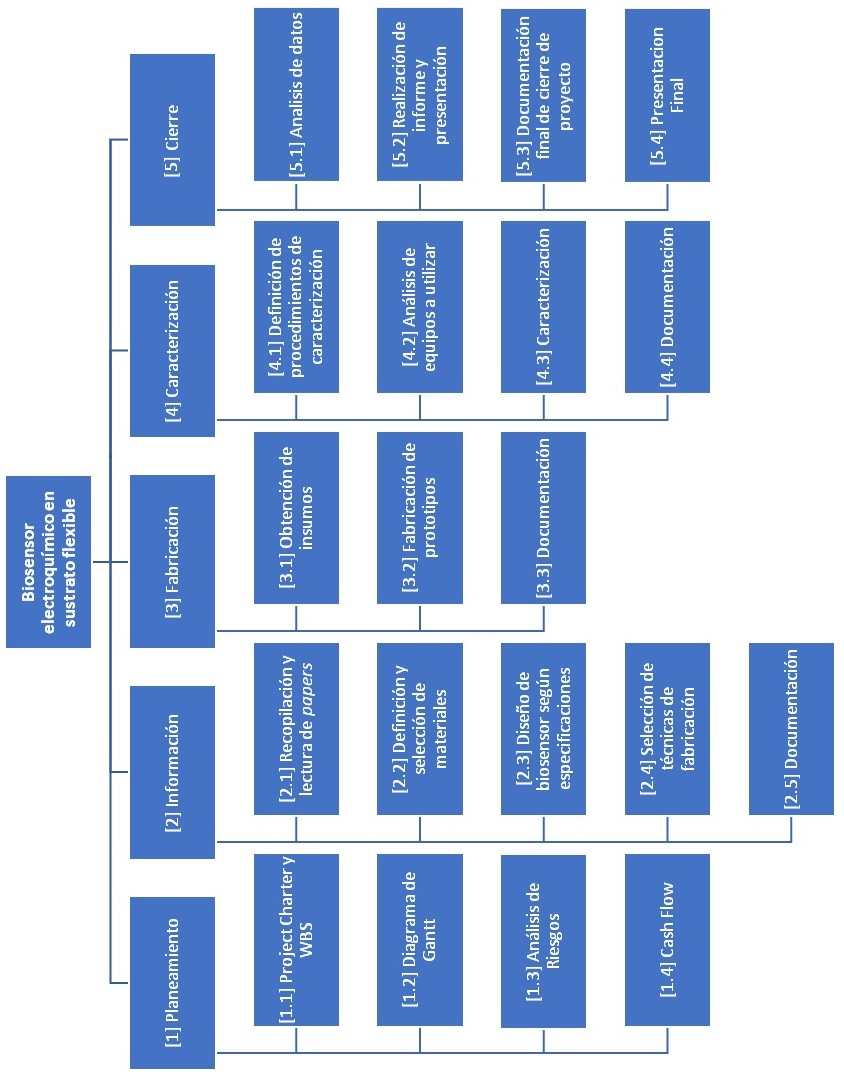
\includegraphics[width=1\textwidth]{Figuras/WBS}
  \label{fig:WBS}
\end{figure}
\newpage 
\begin{flushleft}
{\Large \textbf{Diagrama de Gantt}}
\end{flushleft}
\begin{figure}[H]
  \centering
    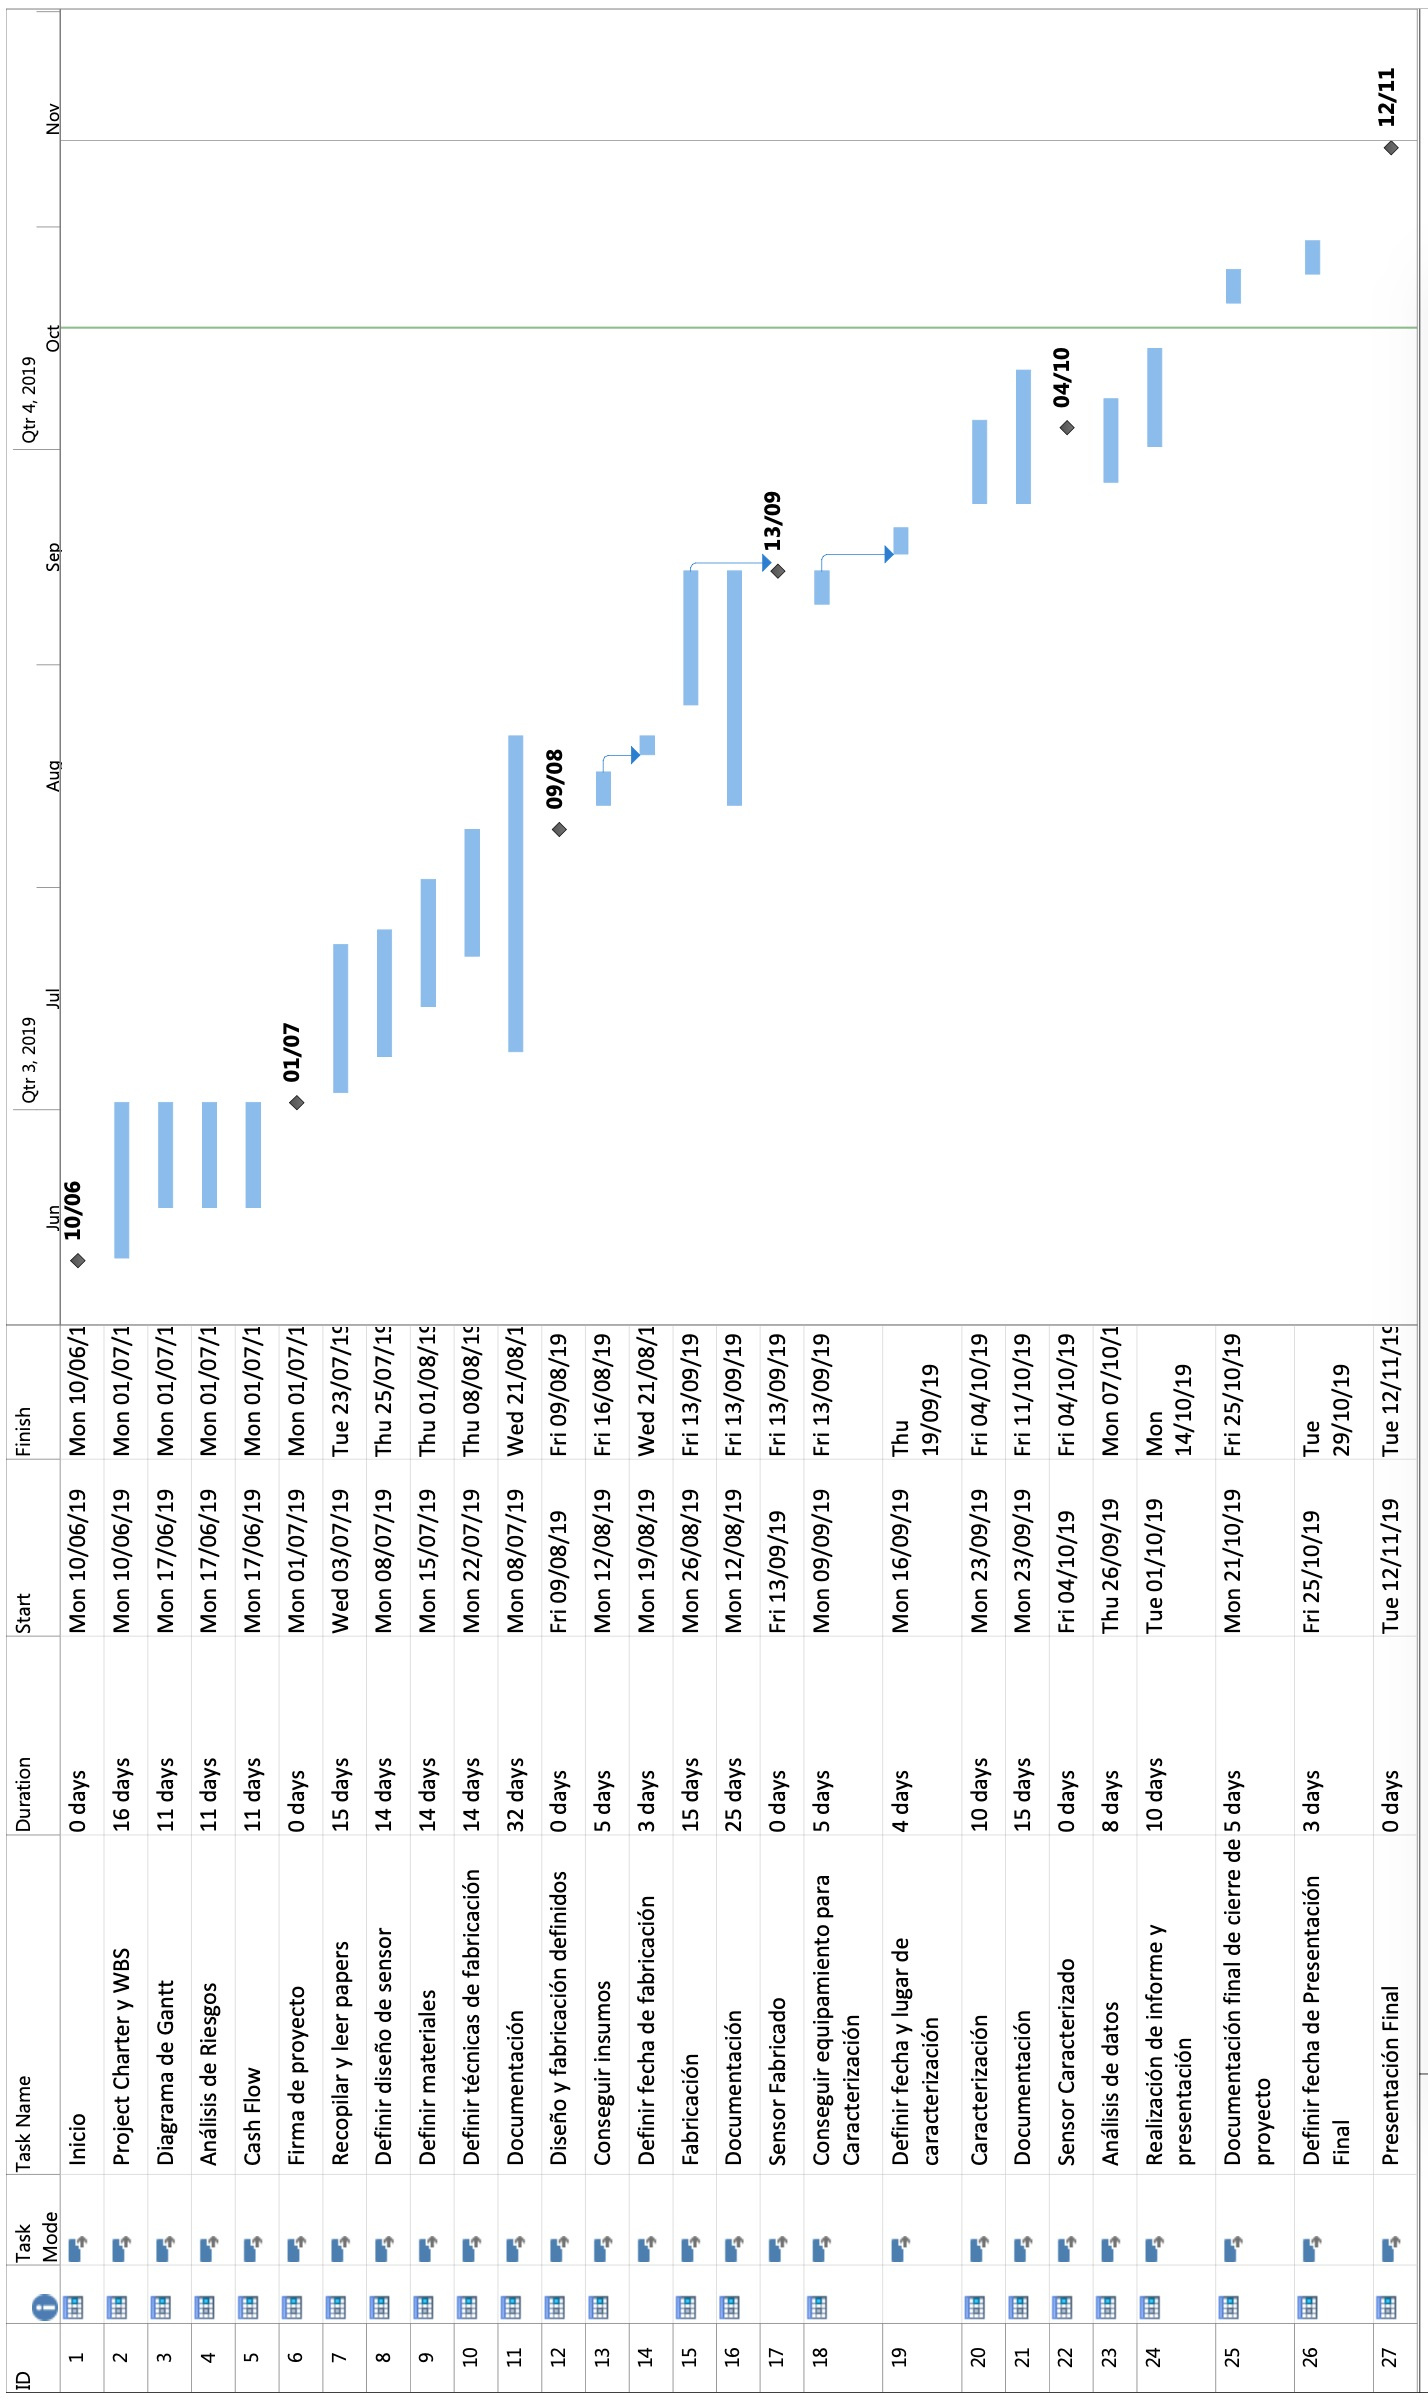
\includegraphics[width=0.82\textwidth]{Figuras/Gantt}
  \label{fig:Gantt}
\end{figure}
\newpage 
\begin{flushleft}
{\Large \textbf{Evaluación de riesgos}}
\end{flushleft}
\begin{figure}[H]
  \centering
    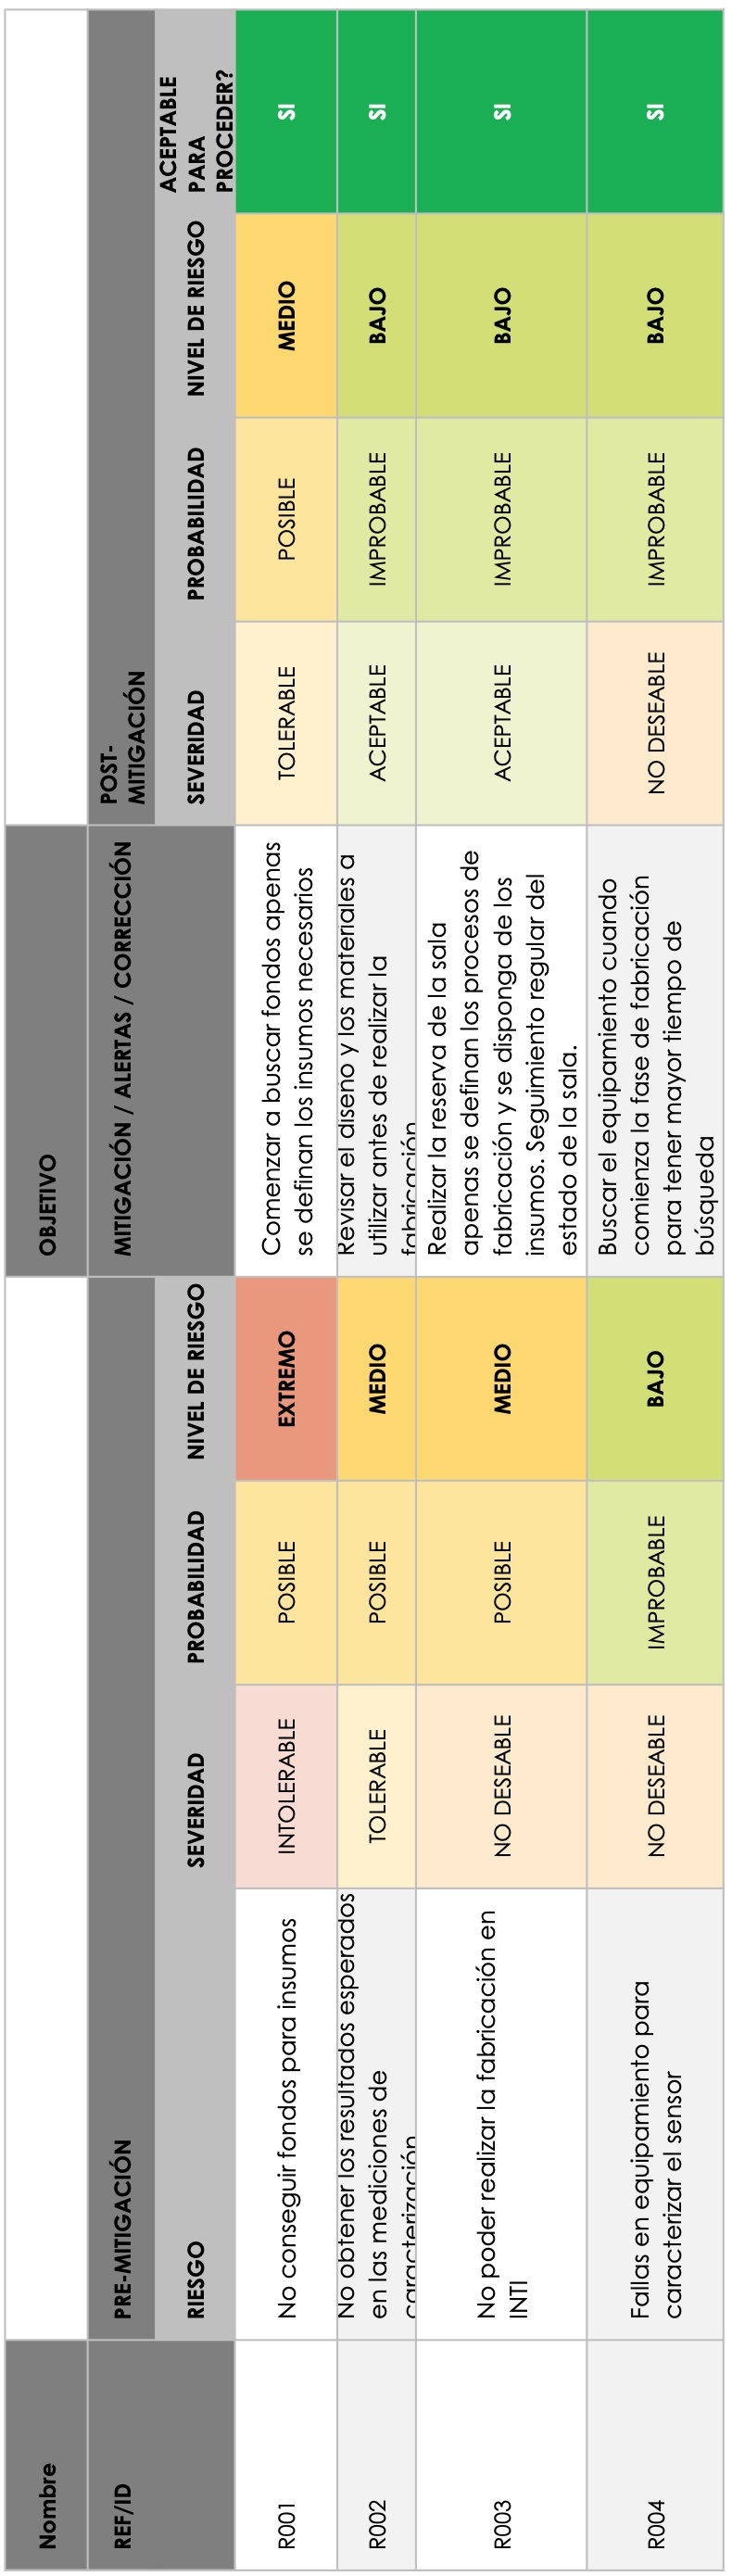
\includegraphics[width=0.38\textwidth]{Figuras/MatRiesgos}
  \label{fig:MatRiesgos}
\end{figure}
\newpage 
\begin{flushleft}
{\Large \textbf{Cashflow}}
\end{flushleft}
\begin{figure}[H]
  \centering
    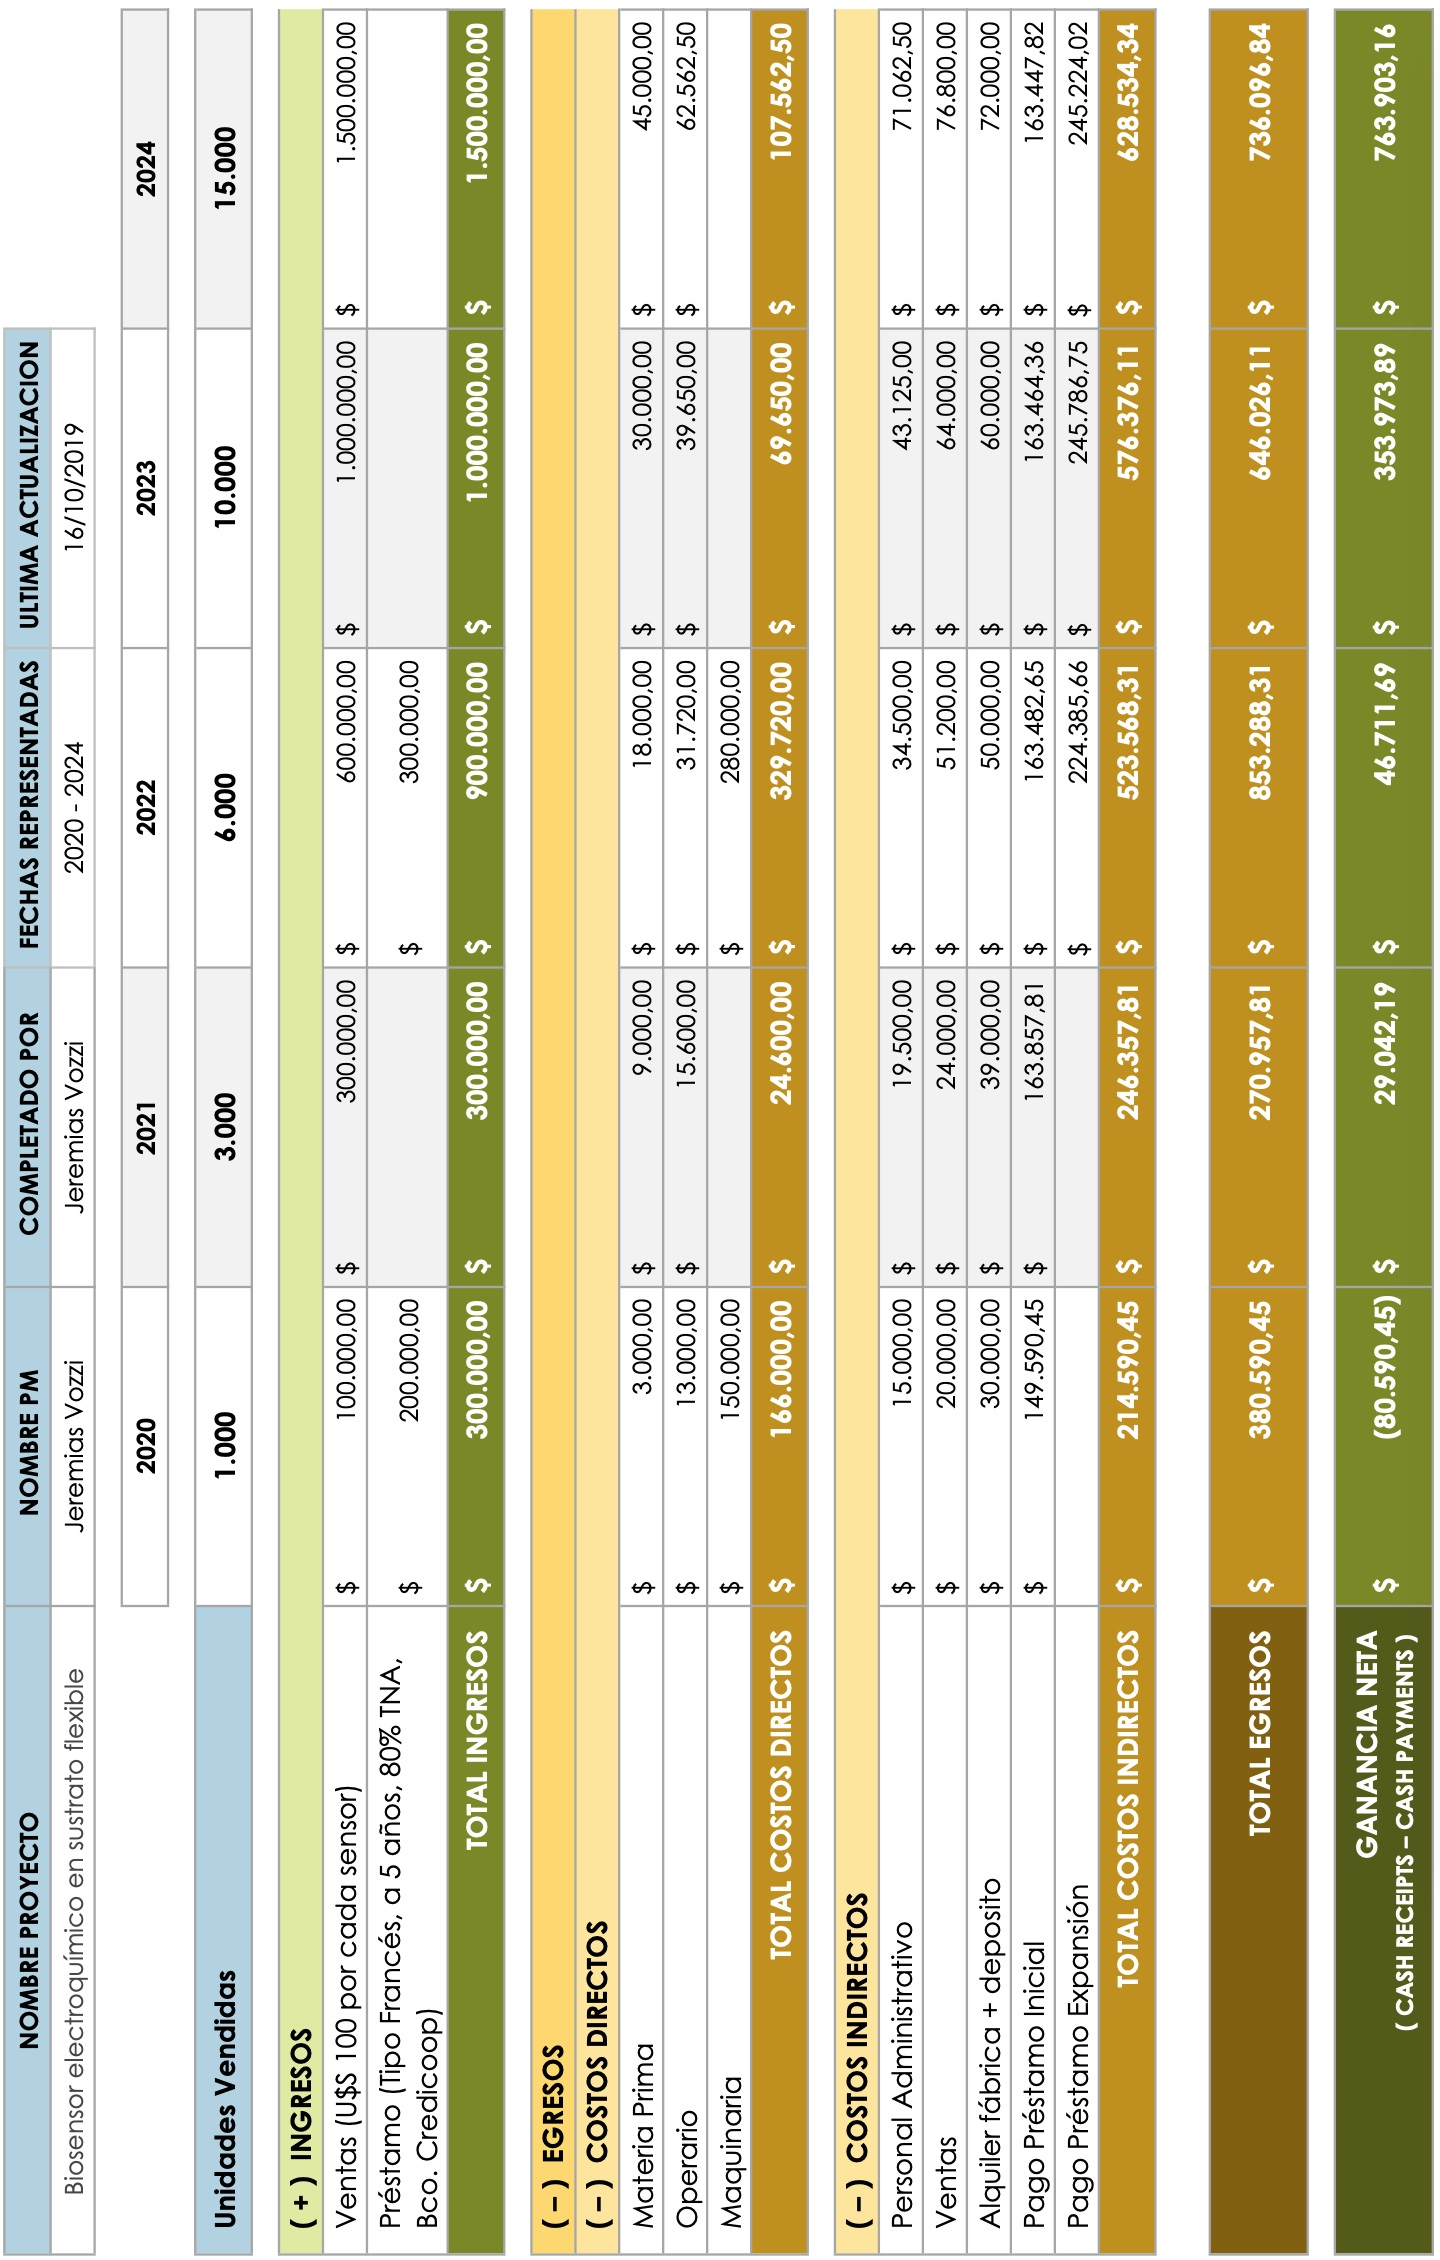
\includegraphics[width=0.85\textwidth]{Figuras/CashFlow}
  \label{fig:CashFlow}
\end{figure}

\begin{flushleft}
{\Large \textbf{Proceso de seguimiento y control}}
\end{flushleft}
Para realizar el seguimiento del proyecto se optó por generar reportes parciales sobre el estado del proyecto, una vez por semana, a través de actualizaciones de avance en el Gantt. Esto se llevo a cabo utilizando el software Project de Microsoft. De esta manera, en conjunto con los tutores, se registró el desempeño semanal teniendo en cuenta los adelantos o atrasos en las tareas y el cumplimiento de los hitos a tiempo. Mediante una reunión por semana, utilizando estos reportes, se actualizaba el cronograma y se planificaba la semana siguiente para cumplir con los objetivos propuestos.

De esta forma, se logró cumplir con los tiempos, costos y alcance estipulados.

\tableofcontents
\listoffigures

\chapter{Objetivos}
El proyecto se basa en el diseño, fabricación y caracterización de un biosensor electroquímico sobre un sustrato flexible a ser utilizado en la plataforma NanoPoc (Figura ~\ref{fig:Figura_Nano_Poc}), desarrollada en el Instituto Nacional de Tecnología Industrial, para la detección de enfermedades bacterianas, virales o parasitarias en salud humana y sanidad animal \cite{PosterPoc2}.

\begin{figure}[H]
  \centering
    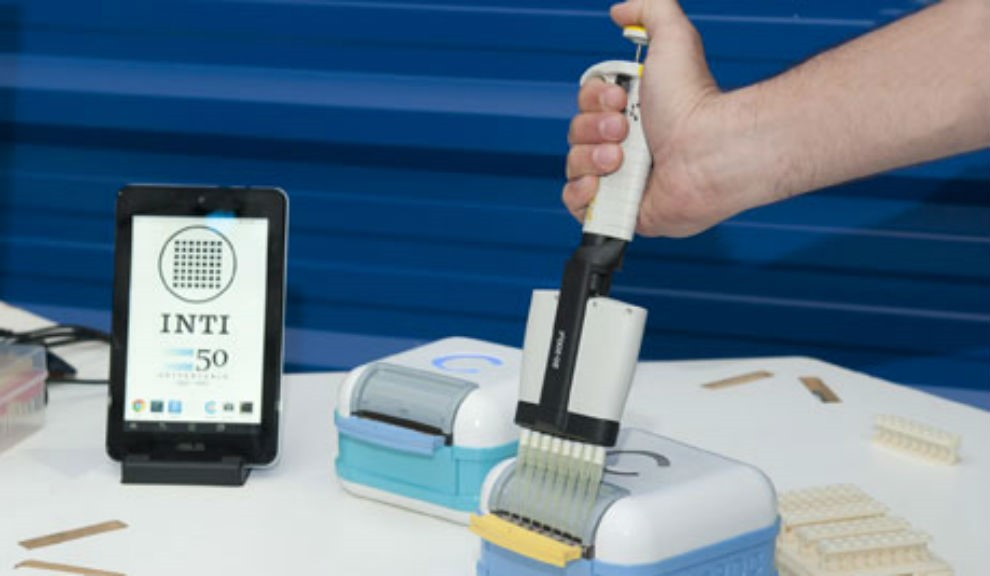
\includegraphics[width=0.5\textwidth]{Figuras/Figura_Nano_Poc}
  \caption{Plataforma NanoPoc.}
  \label{fig:Figura_Nano_Poc}
\end{figure}

\section{Objetivos Generales}
El objetivo principal es generar un biosensor de fácil fabricación y con alta reproducibilidad. Se pretende mejorar el uso del mismo, evitando el manejo de preparación de muestras entre la extracción y la medición en el dispositivo, para la detección $``$\textit{in situ}$"$ de enfermedades infecciosas en humanos y animales, dependiendo del tipo de biorreceptor desarrollado (Figura ~\ref{fig:Figura_Biosensor_objetivos}).
\begin{figure}[H]
  \centering
    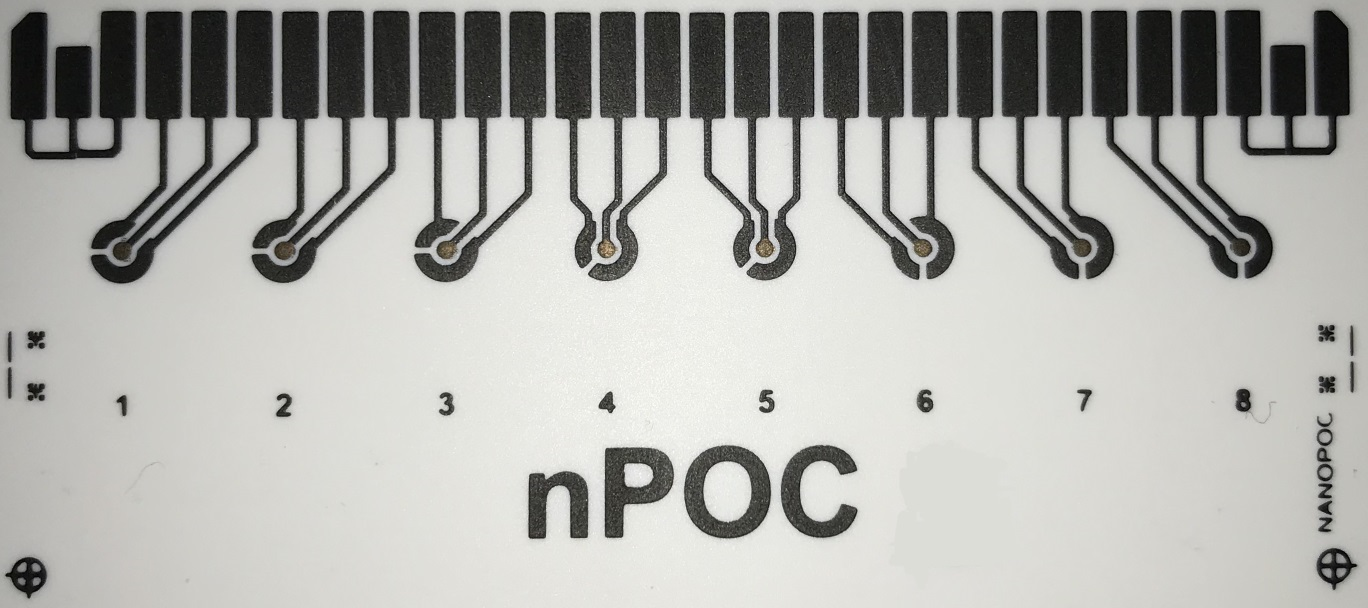
\includegraphics[width=0.5\textwidth]{Figuras/Figura_Biosensor_objetivos}
  \caption{Biosensor.}
  \label{fig:Figura_Biosensor_objetivos}
\end{figure}
\section{Objetivos Espec\'ificos}
- Fabricar los sensores con la forma adecuada, mediante una deposición controlada de material sobre el sustrato flexible, creando 8 celdas electroquímicas con las dimensiones estándar de una micropipeta de 8 canales (Figura ~\ref{fig:Figura_celda_electroquimica}).\\
\begin{figure}[H]
  \centering
    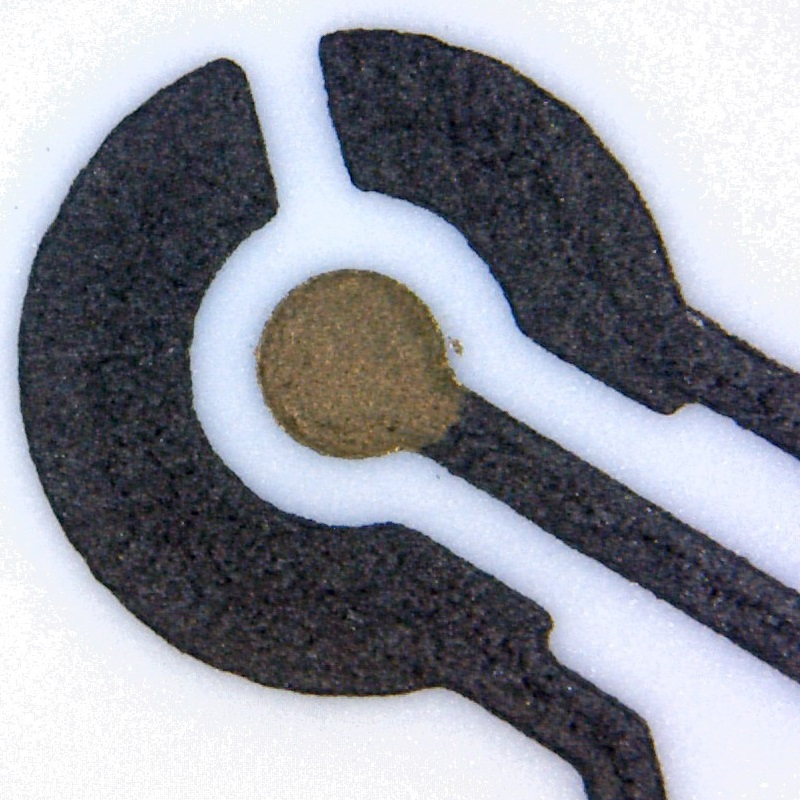
\includegraphics[width=0.35\textwidth]{Figuras/Figura_celda_electroquimica}
  \caption{Celda electroquímica.}
  \label{fig:Figura_celda_electroquimica}
\end{figure}
- Calibrar la impresora \textit{inkjet} con el fin de obtener el diseño del biosensor deseado utilizando una tinta específica sobre el sustrato elegido (Figura ~\ref{fig:Figura_impresora_objetivos}).\\
\begin{figure}[H]
  \centering
    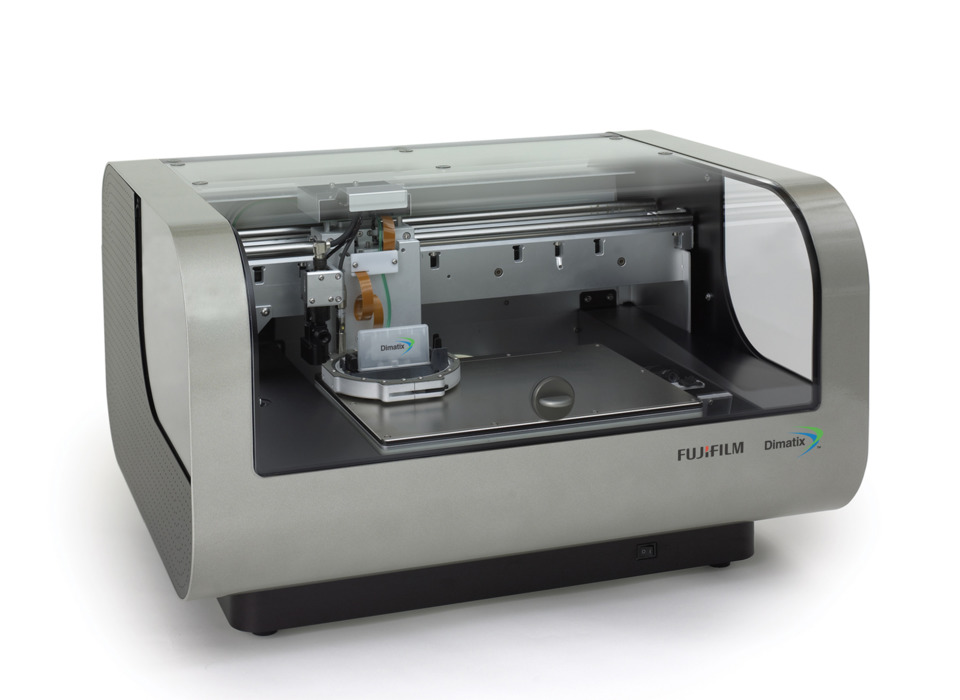
\includegraphics[width=0.5\textwidth]{Figuras/Figura_impresora_objetivos}
  \caption{Impresora \textit{Inkjet}.}
  \label{fig:Figura_impresora_objetivos}
\end{figure}
- Obtener una respuesta correcta de los biosensores mediante una solución química equivalente a un analito específico utilizando la técnica electroquímica del tipo amperométrico (Figura ~\ref{fig:Figura_caracElectroquim_objetivos}).\\
\begin{figure}[H]
  \centering
    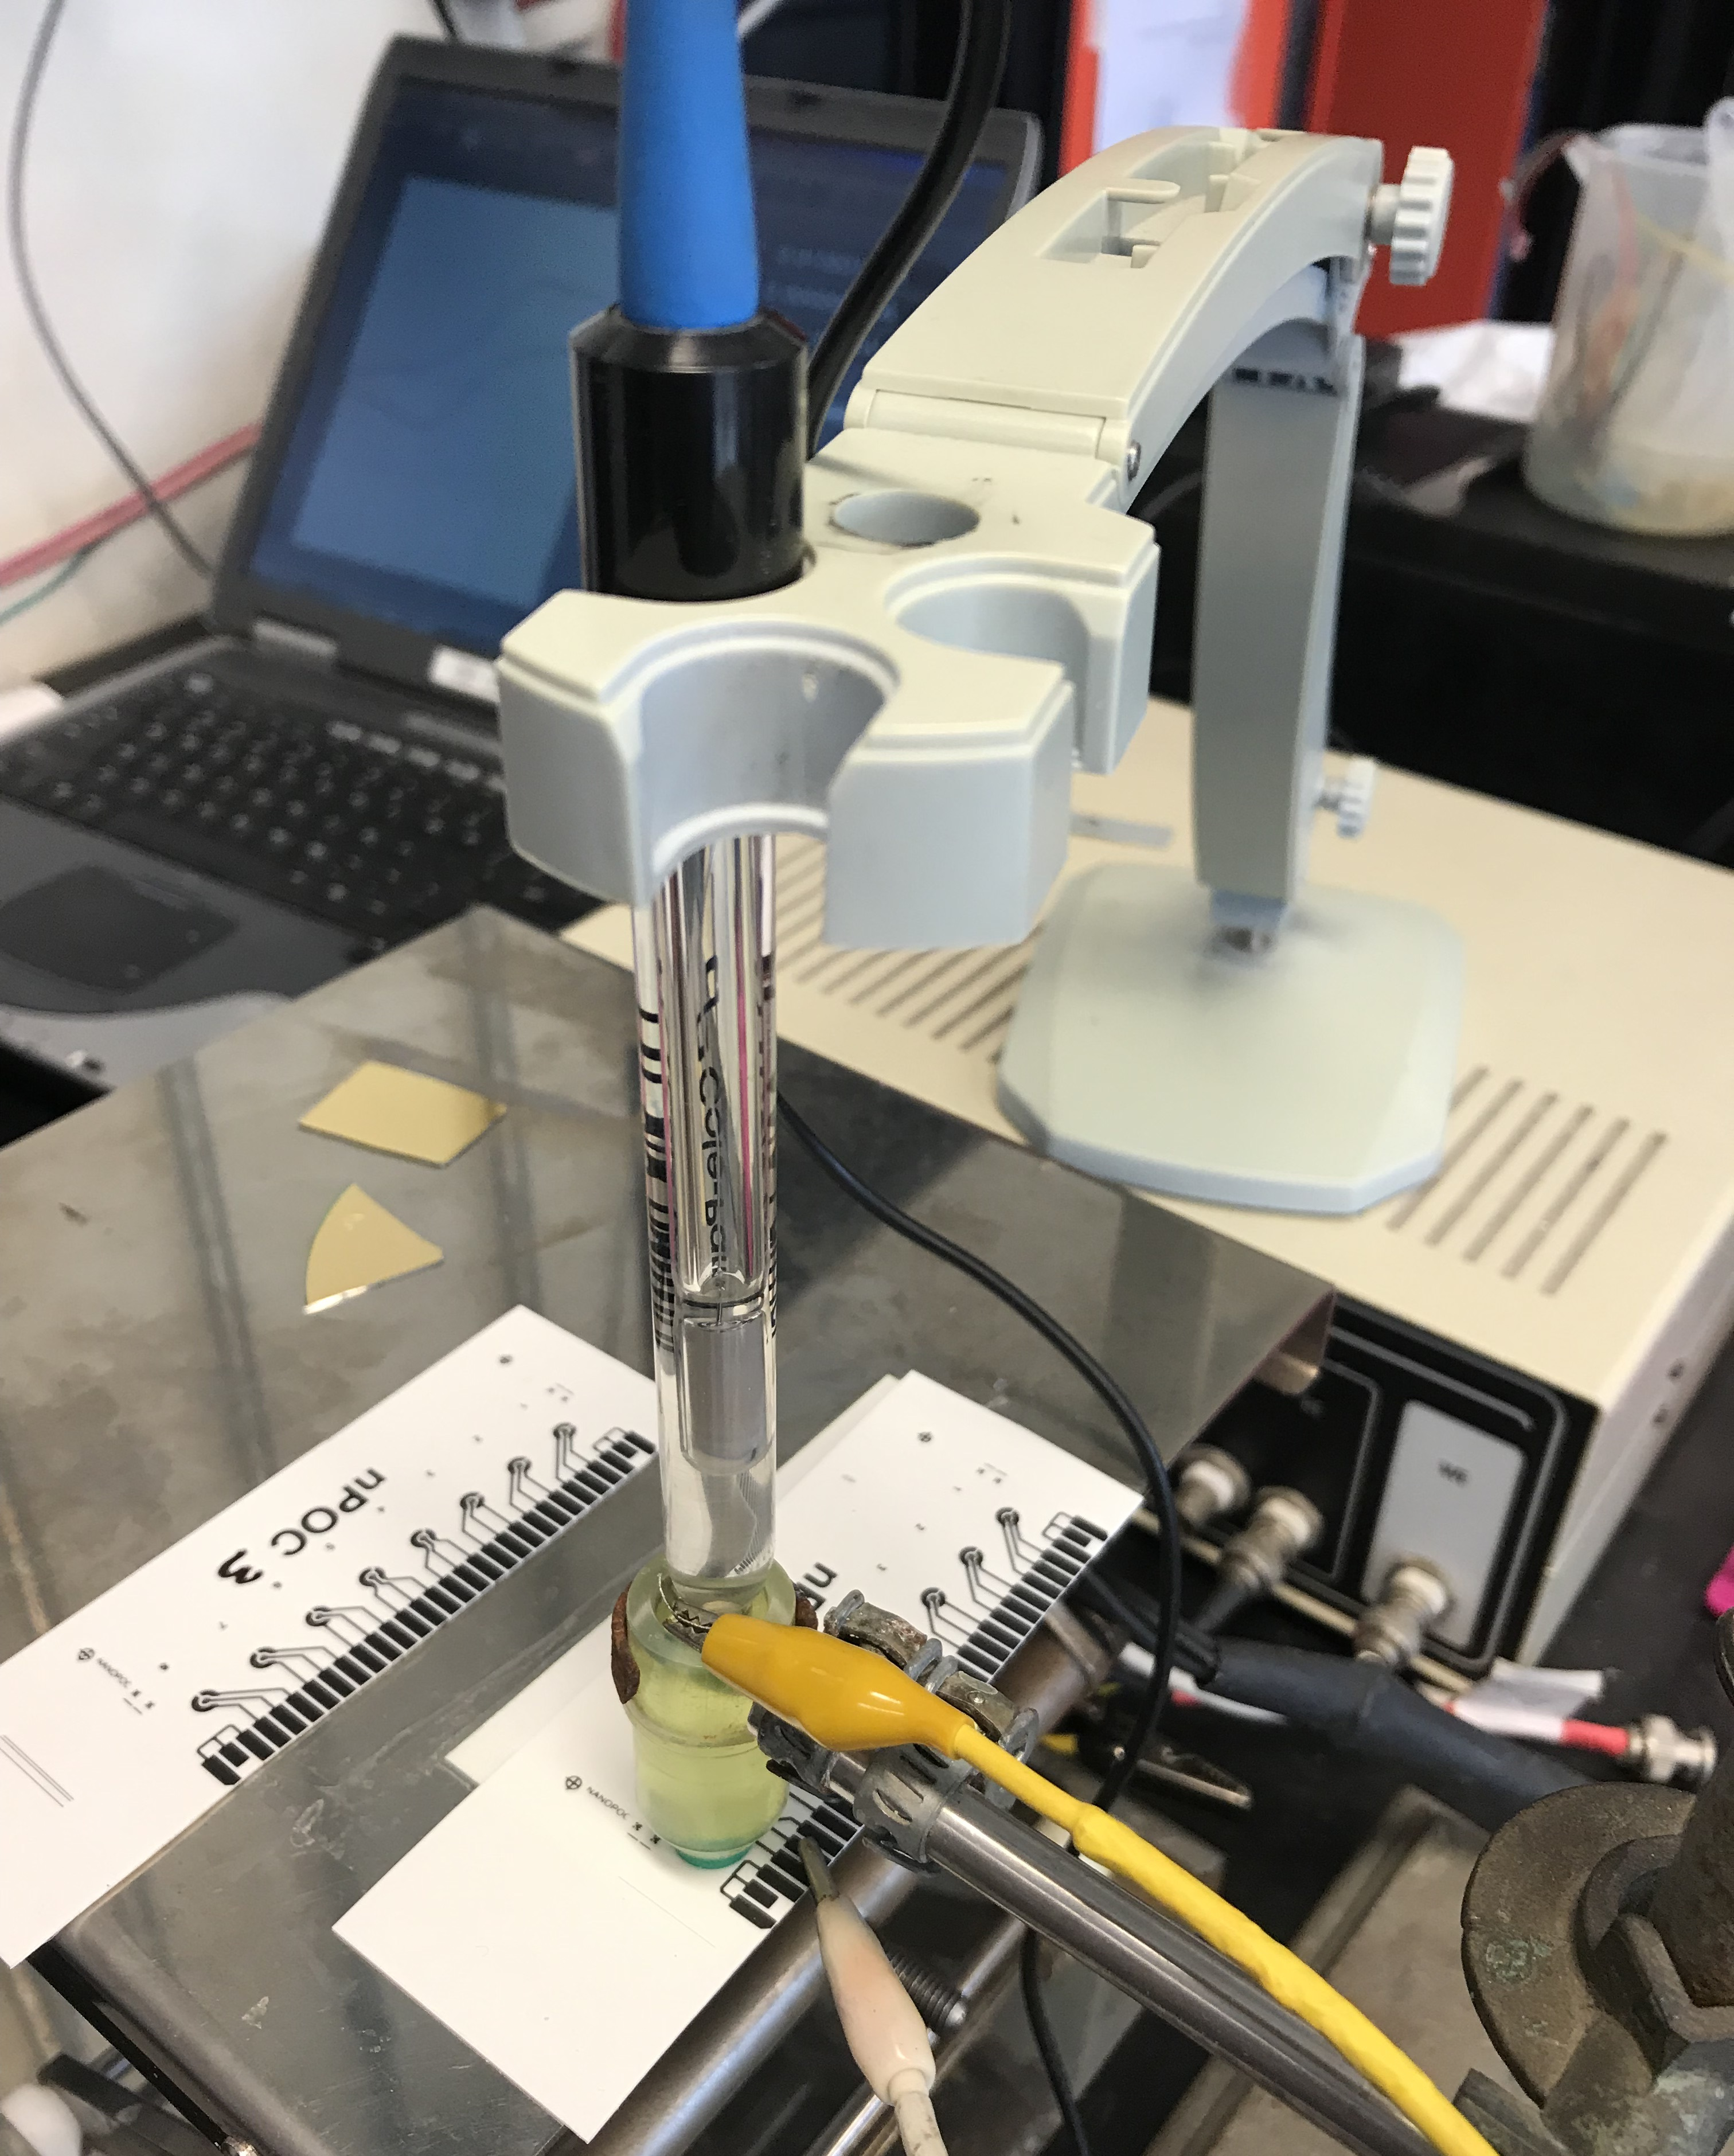
\includegraphics[width=0.4\textwidth]{Figuras/Figura_caracElectroquim_objetivos}
  \caption{Caracterización electroquímica.}
  \label{fig:Figura_caracElectroquim_objetivos}
\end{figure}
\chapter{Marco Te\'orico}
El presente capítulo permite conocer los conceptos básicos necesarios para el entendimiento del desarrollo acorde al proyecto propuesto. El campo de los biosensores se integra de conceptos elementales de electrónica, química, ciencia de los materiales y biología. La electrónica impresa funcional y las impresoras a chorro de tinta precisan de aclaraciones teóricas acordes al proyecto que se desarrollará. Se analizarán principios fundamentales de biosensores, las técnicas de electrónica impresa funcional, la impresión mediante chorro de tinta, los materiales a utilizar y las caracterizaciones a realizar.

\section{Sensores, transductores y biosensores}
Un \textbf{sensor} es un dispositivo capaz de transformar magnitudes físicas o químicas, llamadas variables de instrumentación, en magnitudes eléctricas a través de un transductor. Estos dispositivos pueden ser caracterizados por diferentes propiedades como el rango de medida, la precisión, la linealidad, la repetitividad, entre otros. Las variables de instrumentación pueden ser magnitudes como temperatura, presión, humedad, pH, intensidad lumínica, distancia, aceleración, inclinación, desplazamiento, fuerza, torsión, movimiento, etc. En un significado más extenso, es la ampliación de los sentidos para adquirir un conocimiento de cantidades fisicoquímicas que, por su naturaleza o tamaño, no pueden ser percibidas directamente por los sentidos \cite{PallasAreny}.

Un \textbf{transductor} transforma la variación de la propiedad del sensor en una salida de información detectable por un sistema electrónico. Puede poseer o no un acondicionador de señal dentro del mismo dispositivo, típicamente con alguna de las salidas de uso industrial: salida en tensión (V) o salida normalizada en corriente (4 a 20 mA)(Figura ~\ref{fig:Figura_concepto_sensor}).

\begin{figure}[H]
  \centering
    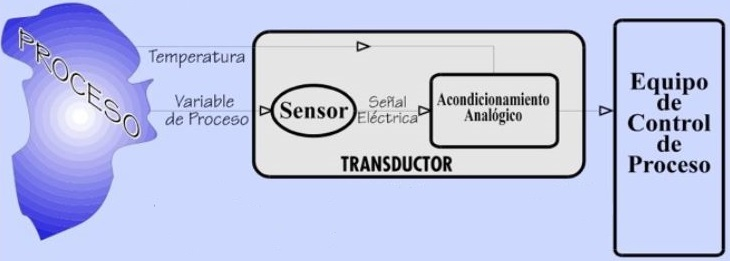
\includegraphics[width=0.8\textwidth]{Figuras/Figura_concepto_sensor}
  \caption{Diagrama sensor y transductor. Figura extraída de \cite{Hector1}.}
  \label{fig:Figura_concepto_sensor}
\end{figure}

Un \textbf{biosensor} se puede definir como un dispositivo que reconoce un determinado analito mediante un \textbf{biorreceptor} acoplado a un \textbf{transductor fisicoquímico} que convierte la señal biológica en una señal eléctrica (Figura ~\ref{fig:Figura_Biosensor}), siendo esta señal proporcional al grupo de compuestos que se quiere determinar cualitativa o cuantitativamente. Un analito es el componente de interés analítico de una muestra. En el caso de los biosensores, son ejemplos una molécula de proteína, una toxina, un péptido, una vitamina o un ion metálico. El biorreceptor puede ser una biomolécula simple o compleja (enzimas, anticuerpos, cadenas de ácidos nucleicos), o basado en células (tejidos, organismos) y puede ser tomado de la naturaleza o sintetizado en un laboratorio. El transductor puede ser del tipo resonante, óptico, térmico, transistor de efecto de campo FET (\textit{Field-Effect Transistor}), de ondas acústicas superficiales (\textit{Surface Acoustic Wave}), piezoeléctrico o electroquímico. Dentro de este último se pueden diferenciar los del tipo conductímetro, amperométrico, potenciométrico e impedométrico \cite{Eggins}.

\begin{figure}[H]
  \centering
    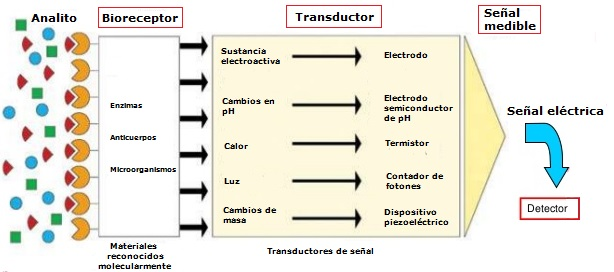
\includegraphics[width=0.8\textwidth]{Figuras/Figura_Biosensor}
  \caption{Diagrama de biosensor: biorreceptor, transductor y acondicionador de señal electrónico. Figura extraída de \cite{Lili1}.}
  \label{fig:Figura_Biosensor}
\end{figure}

Los transductores electroquímicos son los más utilizados en el desarrollo de biosensores enzimáticos. Esto se debe a que poseen una serie de ventajas, tales como:

$\bullet$ Las medidas electroquímicas pueden ser realizadas en volúmenes pequeños, incluso del orden de nanolitros, con relativa facilidad. Esto hace que tales dispositivos sean especialmente apropiados para monitorizar $``$\textit{in vivo}$"$.

$\bullet$ La señal eléctrica obtenida es la transducción directa de la velocidad de reacción química.

$\bullet$ Los límites de detección que se obtienen, normalmente entre 10\textsuperscript{-9} y 10\textsuperscript{-6} mol$\cdot$l\textsuperscript{-1}, son suficientes y adecuados para la detección de numerosos analitos de interés.

$\bullet$ La relativa simplicidad y el bajo costo de la instrumentación electroquímica permiten una fácil disponibilidad de estos dispositivos.


Sin duda alguna, en el contexto de los biosensores electroquímicos, los más prometedores en términos de sensibilidad, selectividad, tamaño, portabilidad y un mínimo volúmen de muestra (analito) necesaria, son los biosensores amperométricos, objeto de estudio del presente proyecto final integrador. Dichos sensores monitorizan corrientes faradaicas (transferencia directa de electrones vía una reacción de oxidación en un electrodo y una reacción de reducción en el otro) entre el sistema biológico y una celda electroquímica típica conformada por tres electrodos: un electrodo de trabajo \emph{(WE)}, uno de referencia \emph{(RE)} y un contra electrodo \emph{(CE)} (Figura ~\ref{fig:Figura_Definicion_Electrodo}). En el \emph{WE} ocurre la reacción electroquímica, para lo cual se le aplica un potencial variable respecto del electrodo de potencial fijo \emph{(RE)}. La corriente resultante de la reacción química circula entre el \emph{WE} y el \emph{CE}. La variación de potencial aplicado y la medición de corriente se controlan mediante un potenciostato.

\begin{figure}[H]
  \centering
    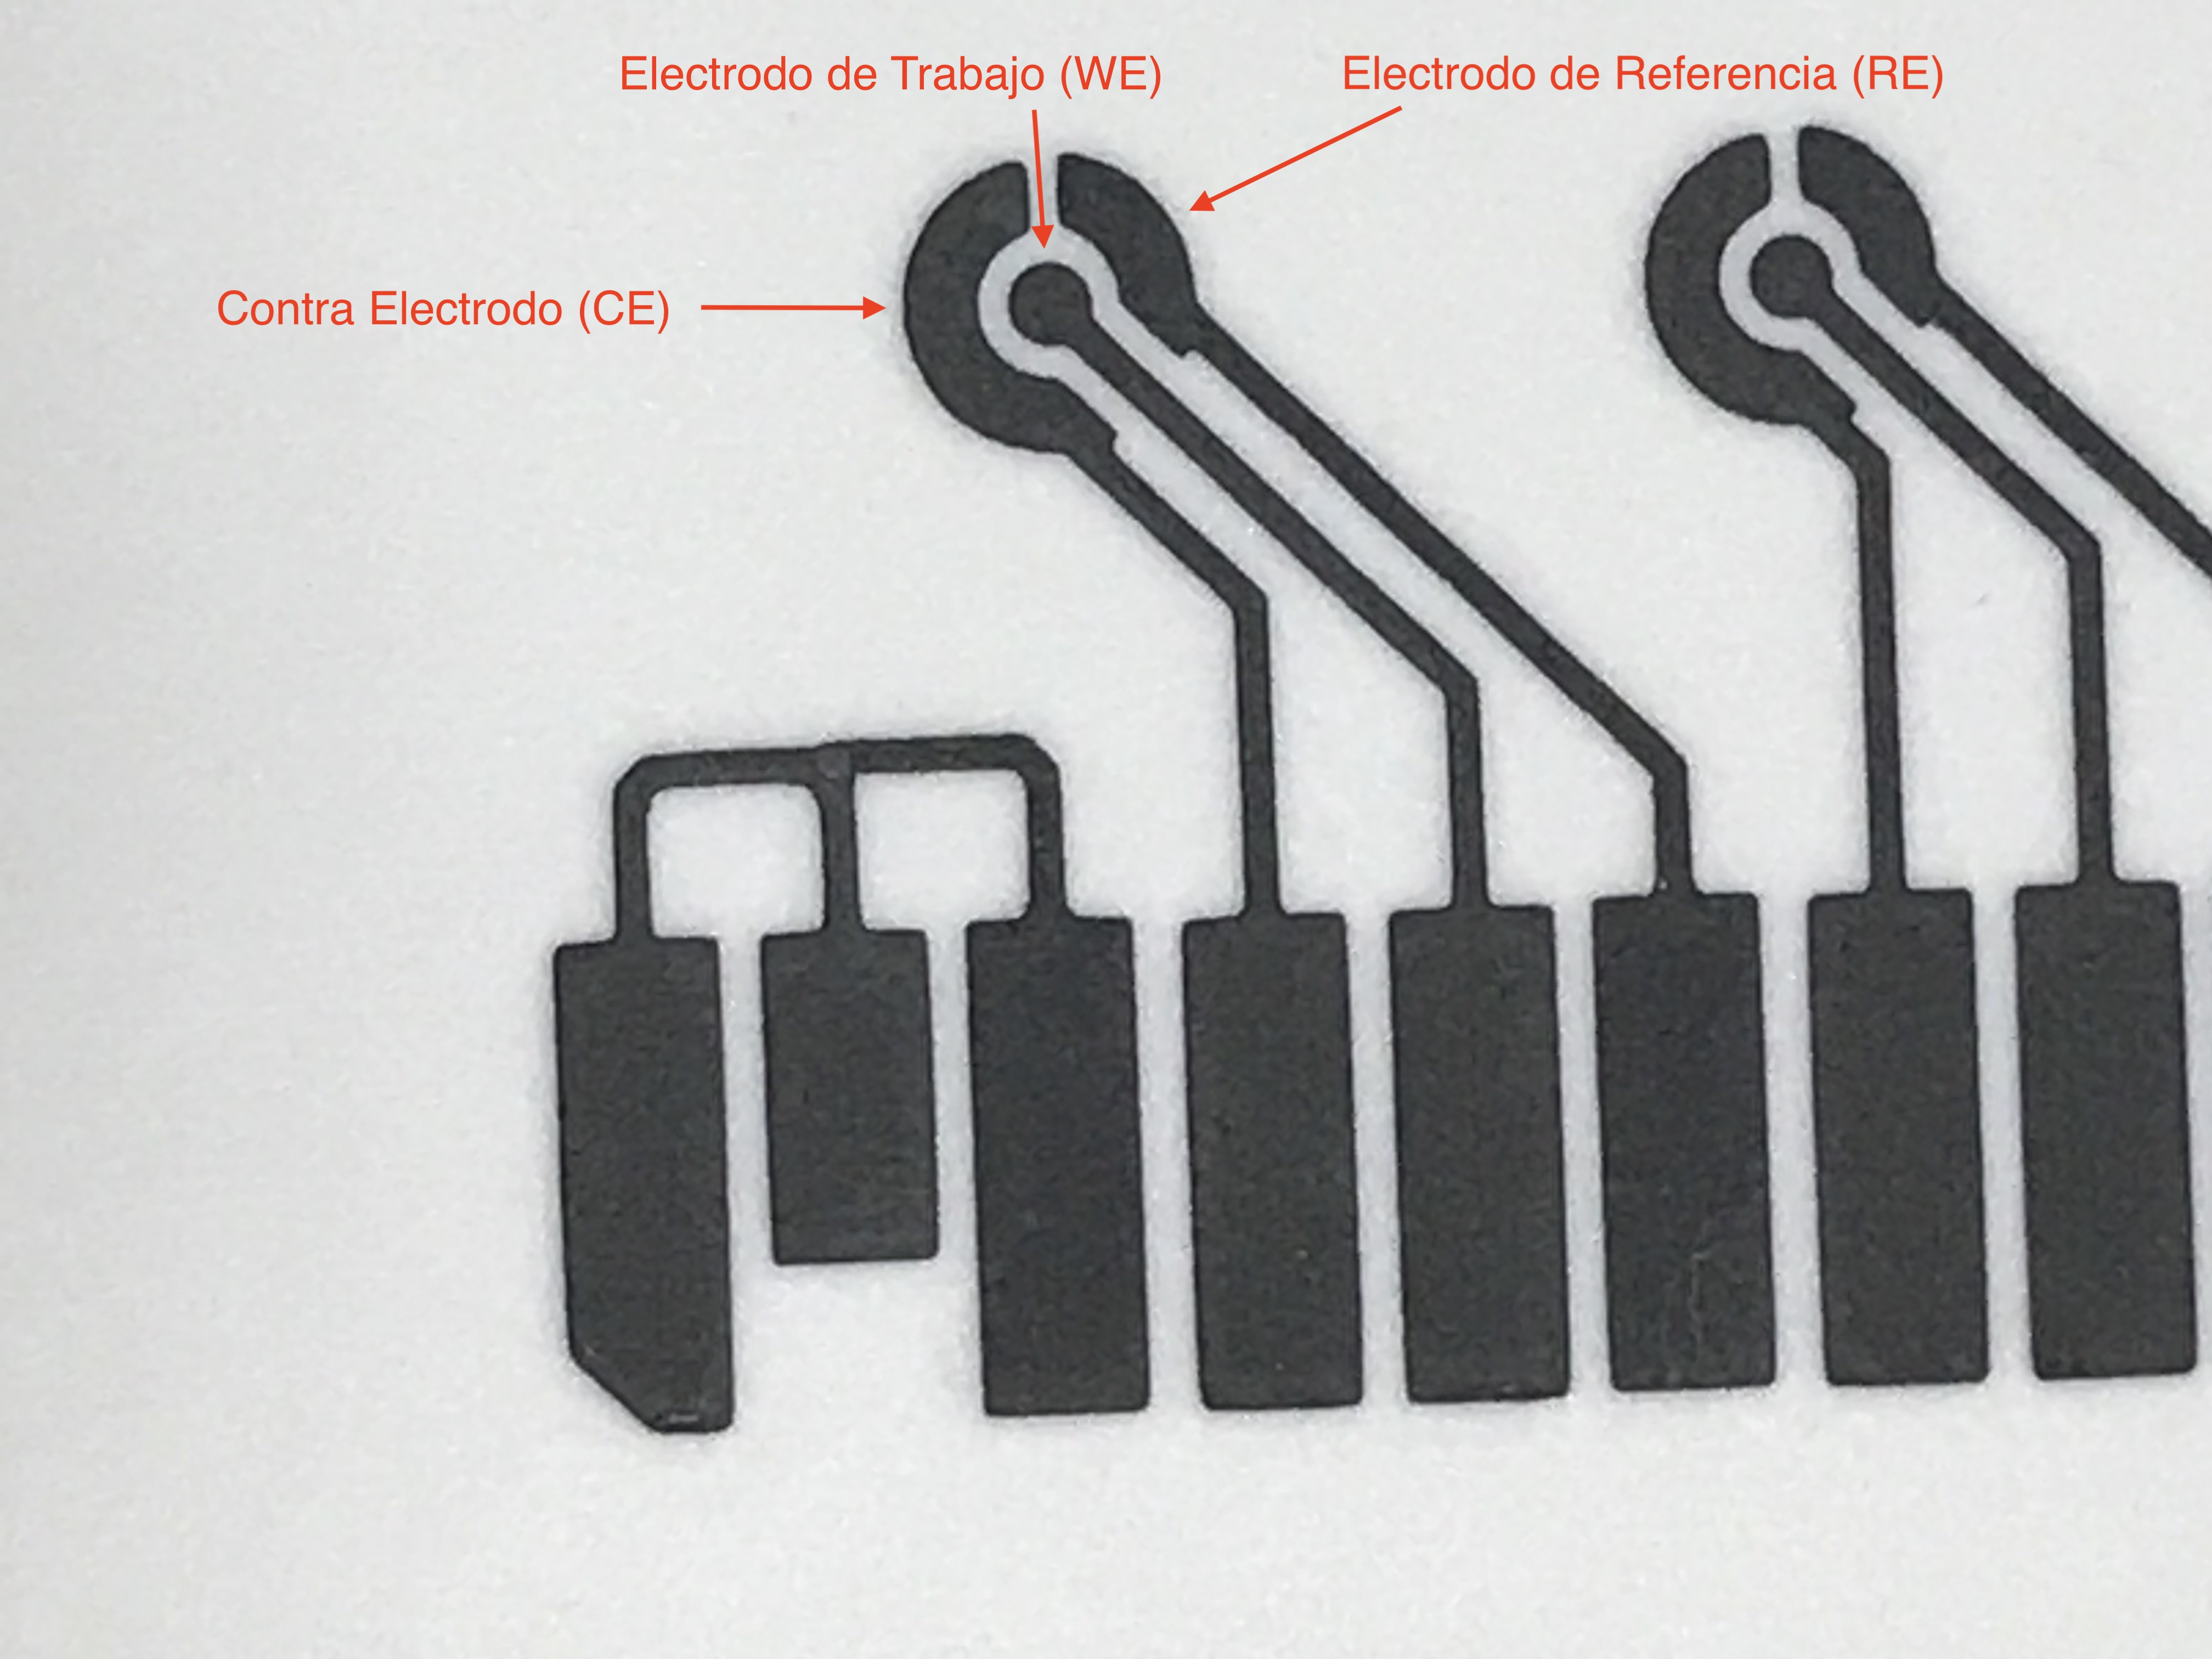
\includegraphics[width=0.5\textwidth]{Figuras/Figura_Definicion_Electrodo}
  \caption{Biosensor Electroquímico.}
  \label{fig:Figura_Definicion_Electrodo}
\end{figure}

Un potenciostato (Figura ~\ref{fig:Figura_potenciostato}) es un dispositivo electrónico utilizado para controlar una celda de tres electrodos y poder realizar la mayoría de los experimentos electroanalíticos. Su función es aplicar un potencial variable sobre el \emph{WE} respecto del potencial fijo aplicado sobre el \emph{RE} y medir la corriente resultante que circula entre el \emph{WE} (donde ocurre la reacción electroquímica) y el \emph{CE}.

\begin{figure}[H]
  \centering
    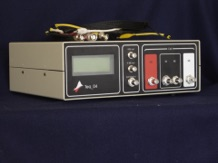
\includegraphics[width=0.5\textwidth]{Figuras/Figura_potenciostato}
  \caption{Potenciostato utilizado para la caracterización electroquímica.}
  \label{fig:Figura_potenciostato}
\end{figure}

\section{Electr\'onica Impresa Funcional}
Aprovechando los avances tecnológicos en micro y nano electrónica, se decidió implementar los biosensores utilizando técnicas de impresión, buscando de esta manera contar con cartuchos de arreglos de sensores descartables, de simple fabricación y alta escala de producción. Dichos biosensores se pueden imprimir sobre sustratos cerámicos (Al\textsubscript{2}O\textsubscript{3}), acrílicos o PMMA (Polímero de Metil Metacrilato), o sobre material flexible tipo PET (PoliEtileno Tereftalato), Valox, etc., utilizando diferentes técnicas, tales como impresión serigráfica ($``$\textit{Screen Printing}$"$) o impresión a chorro de tinta ($``$\textit{Inkjet}$"$).

La impresión serigráfica, propia de la tecnología de película gruesa, permite fabricar circuitos electrónicos y sensores que se obtienen al depositar capas de tintas (típicamente resistivas, conductoras y dieléctricas), por medio de una espátula de goma que se desplaza transversalmente a través de una malla o máscara, con un patrón dado, sobre un sustrato aislado, generalmente cerámica. La espátula fuerza la tinta a atravesar las aberturas de la malla que es de acero inoxidable. Posteriormente se sinterizan a temperaturas pico de 850ºC para remover los solventes de las tintas, fijar las características eléctricas de las tintas y adherir las capas al sustrato (Figura ~\ref{fig:Figura_serigrafia}).

\begin{figure}[H]
  \centering
    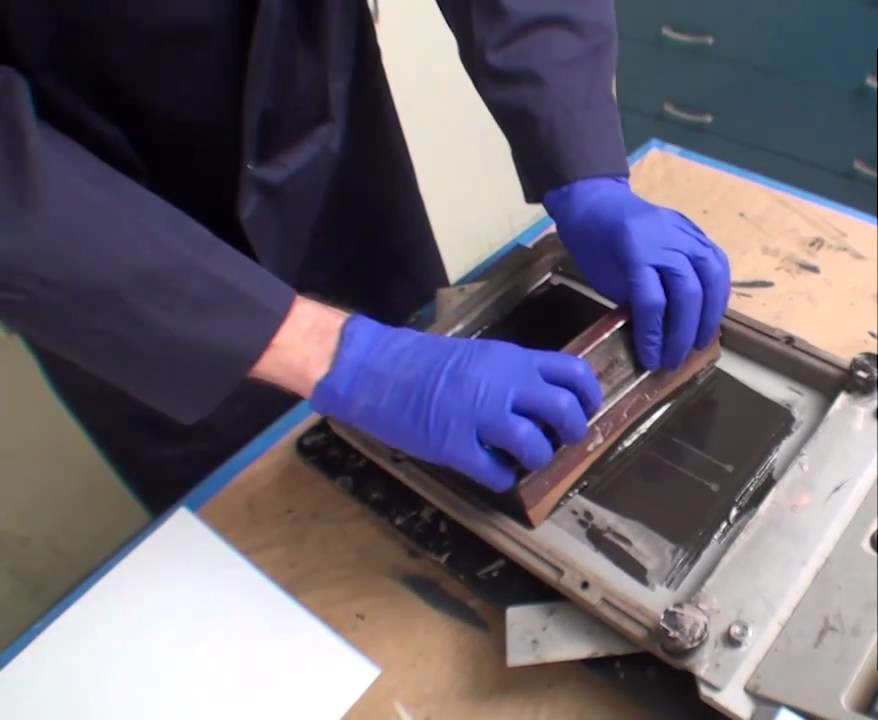
\includegraphics[width=0.5\textwidth]{Figuras/Figura_serigrafia}
  \caption{Impresión serigráfica manual.}
  \label{fig:Figura_serigrafia}
\end{figure}


La impresión a chorro de tinta utiliza cabezales piezoeléctricos para depositar gotas de tinta según coordenadas controladas por software. Las tintas pueden ser conductoras, semiconductoras o dieléctricas (Figura ~\ref{fig:Figura_inkjet_dimatix}).

\begin{figure}[H]
  \centering
    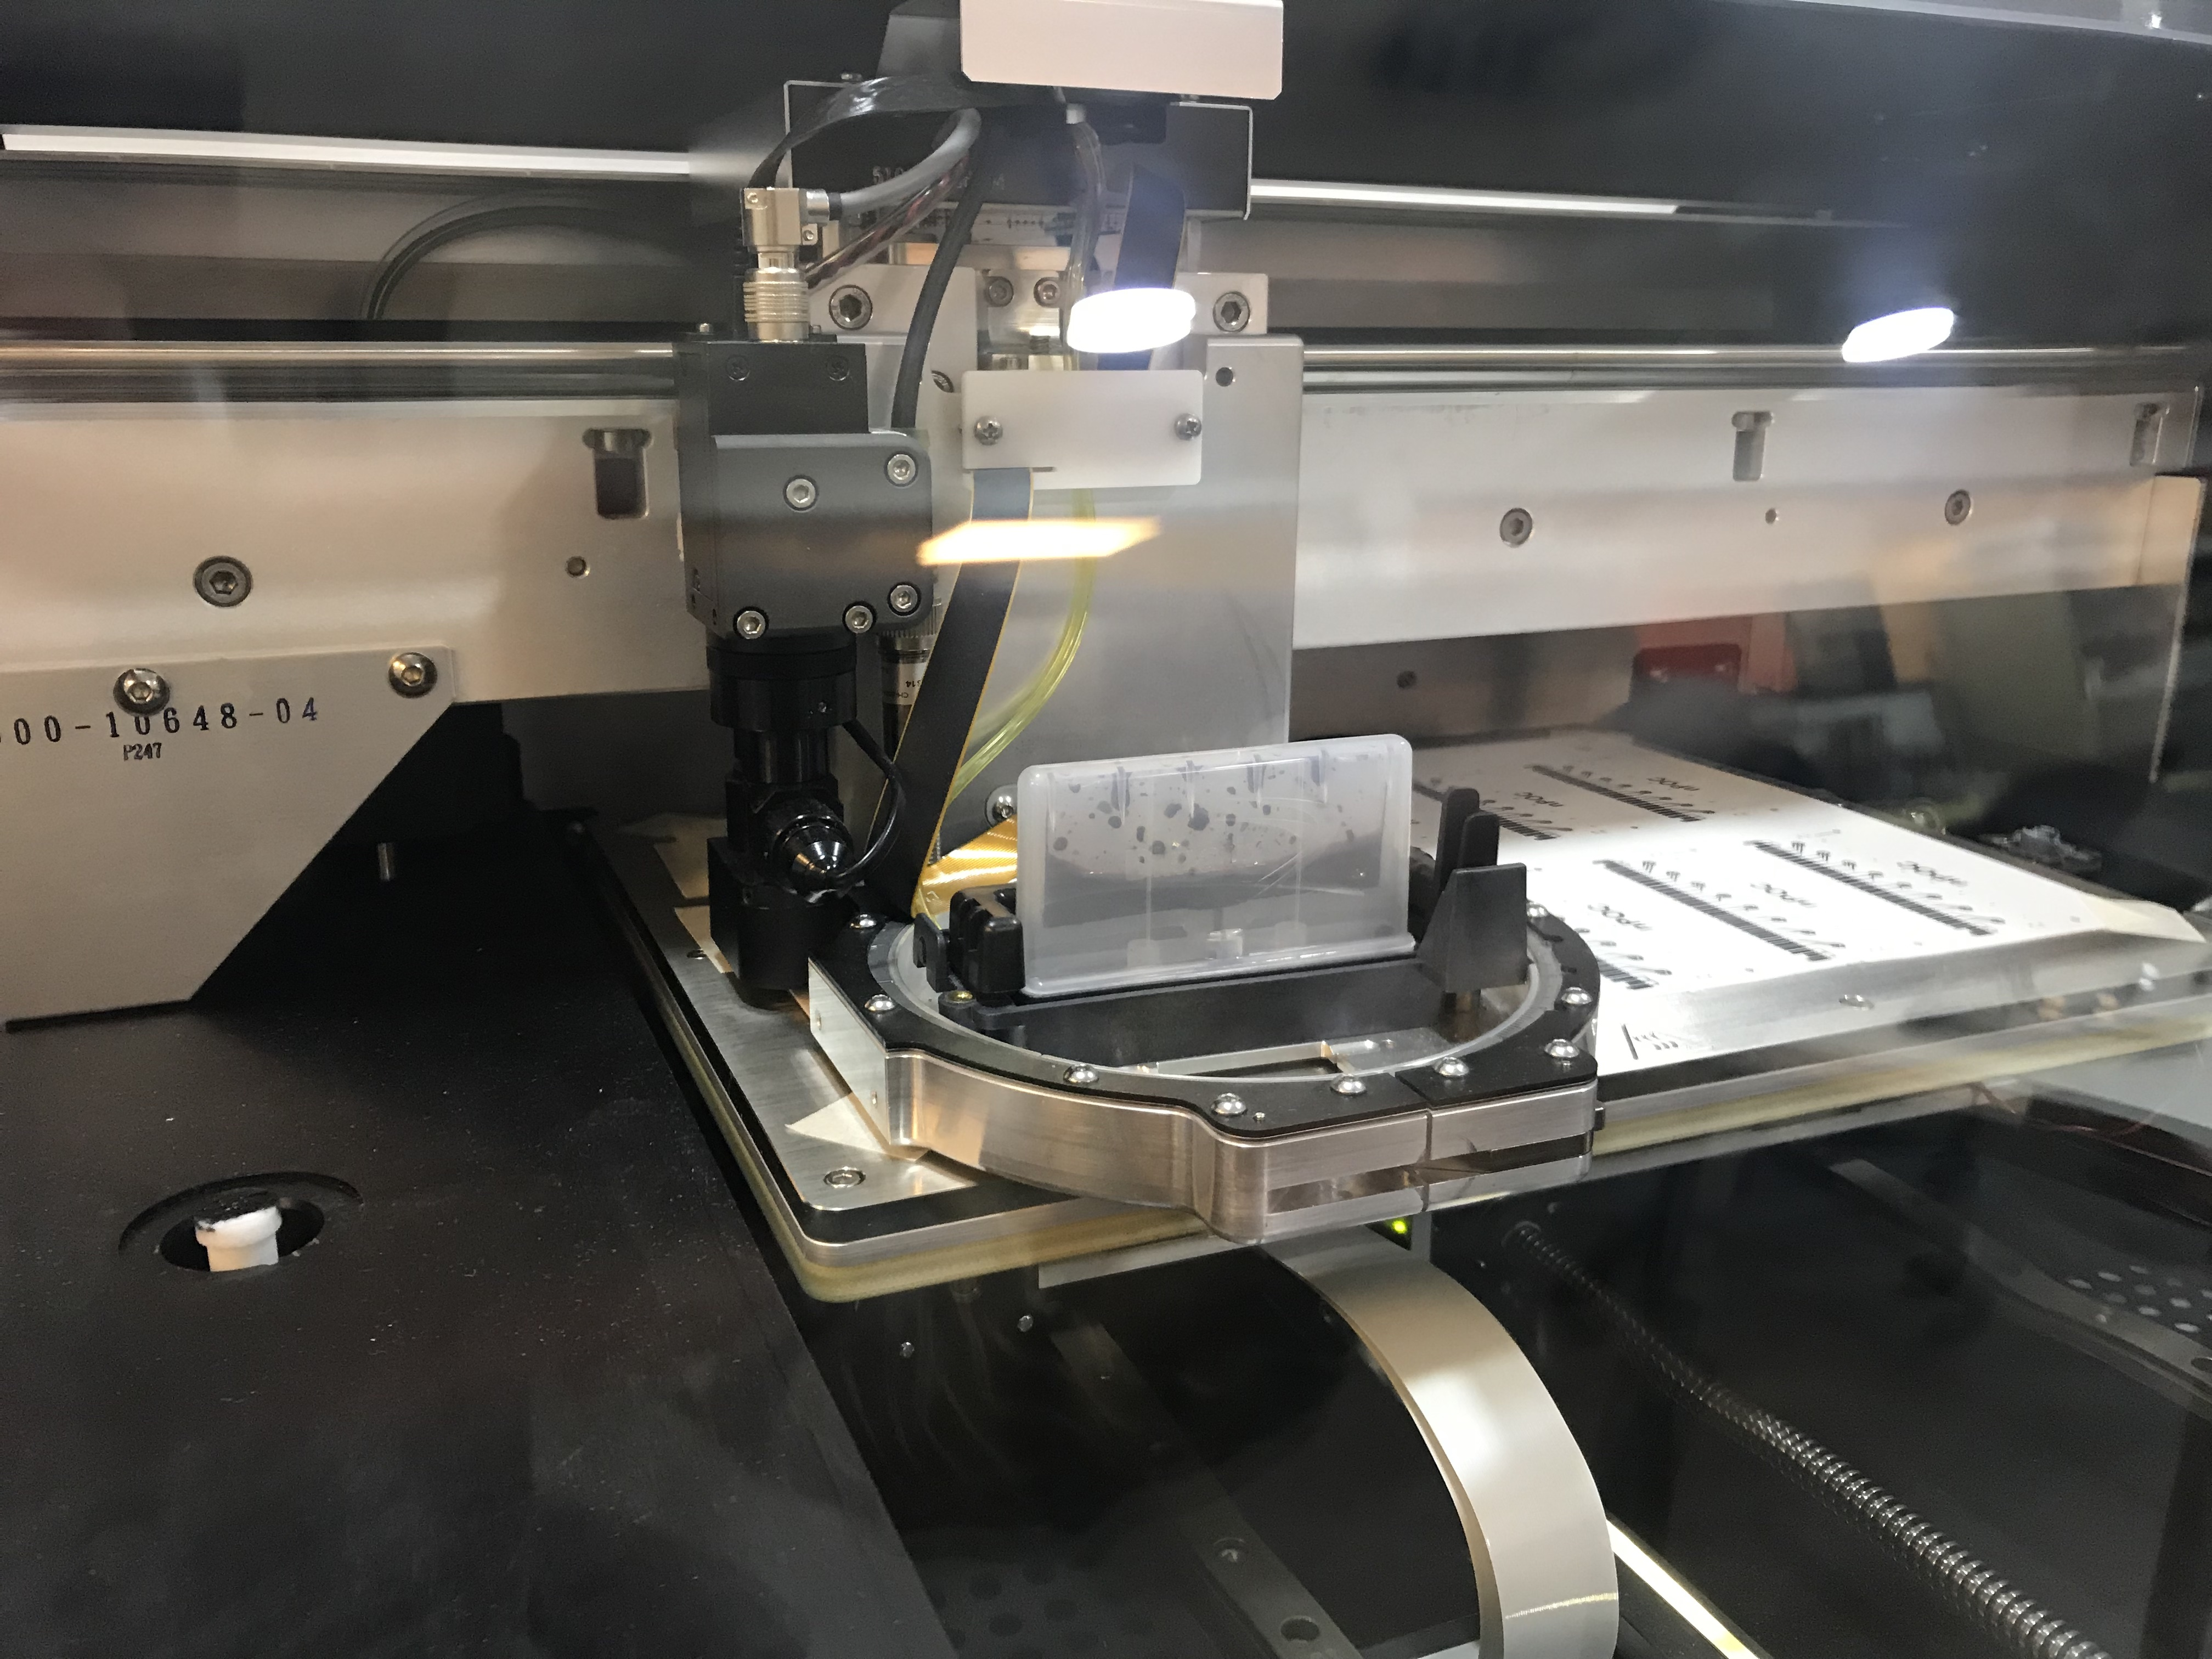
\includegraphics[width=0.5\textwidth]{Figuras/Figura_inkjet_dimatix}
  \caption{Impresión a chorro de tinta.}
  \label{fig:Figura_inkjet_dimatix}
\end{figure}


En esta tesis se implementa un biosensor electroquímico sobre sustrato flexible mediante una impresora \textit{Inkjet} y se utiliza el método amperométrico para caracterizarlo. La versatilidad, facilidad de uso y el tipo de fabricación innovador son algunas de las razones más destacables por las que se decidió realizar el presente proyecto en una impresora de chorro de tinta.

\subsection{Impresora tipo \textit{Inkjet}}
Como se mencionó la impresora tipo \textit{Inkjet} utiliza un cabezal piezoeléctrico para la deposición de tintas (Figura ~\ref{fig:Figura_Piezoelectrico}). Dicho cabezal contiene un reservorio con un cristal que, al aplicársele un potencial, se mueve generando una fuerza mecánica en el tanque, lo que provoca la eyección de una gota de tinta.

\begin{figure}[H]
  \centering
    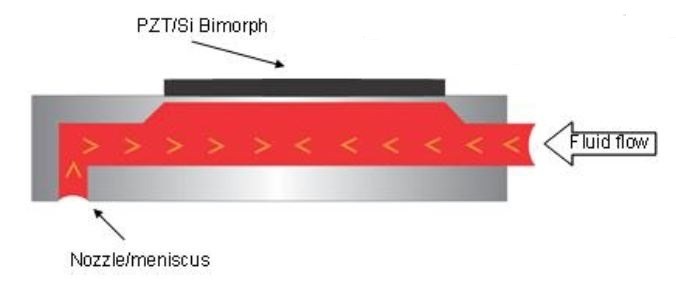
\includegraphics[width=0.5\textwidth]{Figuras/Figura_Piezoelectrico}
  \caption{Esquema de cabezal Piezoeléctrico.}
  \label{fig:Figura_Piezoelectrico}
\end{figure}

Para ello, se debe aplicar una forma de onda especificada por el fabricante (Figura ~\ref{fig:Figura_Waveform_Dimatix}), aunque esta debe ser modificada para cada tipo de tinta. 

\begin{figure}[H]
  \centering
    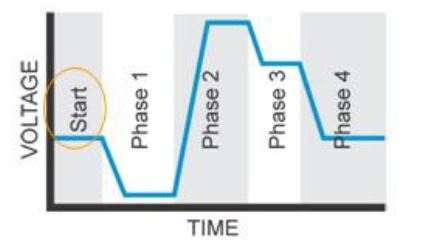
\includegraphics[width=0.5\textwidth]{Figuras/Figura_Waveform_Dimatix}
  \caption{Forma de onda especificada para cabezal de impresión piezoeléctrico.}
  \label{fig:Figura_Waveform_Dimatix}
\end{figure}

En la etapa denominada $``$\textit{Start}$"$ o también identificada como $``$\textit{Standby}$"$, el piezoeléctrico está levemente deflectado generando un menisco de tinta, evitando la caída involuntaria de tinta. En la etapa $``$\textit{Phase 1}$"$ se disminuye el potencial y el piezoeléctrico se mueve hacia arriba, permitiendo el llenado del reservorio. En la etapa $``$\textit{Phase 2}$"$ se incrementa la tensión, iniciando la formación de la gota. Una vez formada la gota, en la etapa $``$\textit{Phase 3}$"$ se vuelve a disminuir la tension, desprendiéndose la gota del cabezal. La etapa $``$\textit{Phase 4}$"$ es el retorno a la tensión de $``$\textit{Start}$"$ (Figura ~\ref{fig:Figura_etapas_eyector}).

\begin{figure}[H]
  \centering
    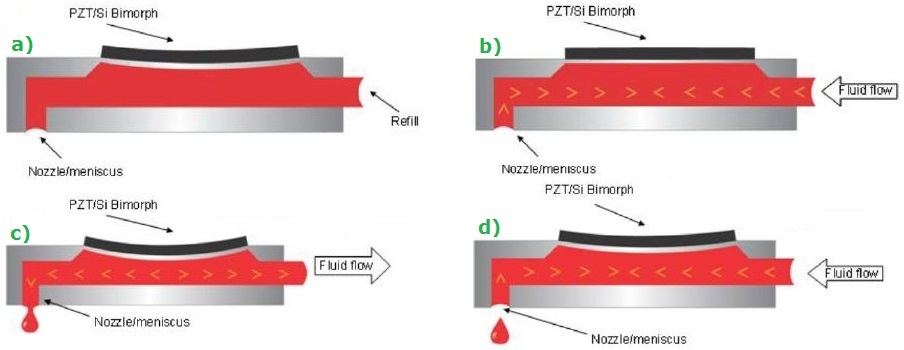
\includegraphics[width=0.8\textwidth]{Figuras/Figura_etapas_eyector}
  \caption{a) Etapa Start/Standby, b) Etapa 1, c) Etapa 2, d) Etapa 3 y vuelta a Standby.}
  \label{fig:Figura_etapas_eyector}
\end{figure}

Los parámetros modificables de esta forma de onda son el nivel de tensión (porcentaje relativo a la tensión seteada al eyector), velocidad de subida (\textit{Slew rate}) que especifica la pendiente de las rampas entre fases y la duración de cada segmento \cite{DimatixUM}.

El cabezal, responsable de eyectar la tinta es una pieza del tipo \textit{MEMS} (Sistemas-Micro-Electro-Mecánicos). Debido a esto son del tamaño convencional de una impresora de inyección térmica, pero de una tecnología superior (Figura ~\ref{fig:Figura_cabezal}). 

\begin{figure}[H]
  \centering
    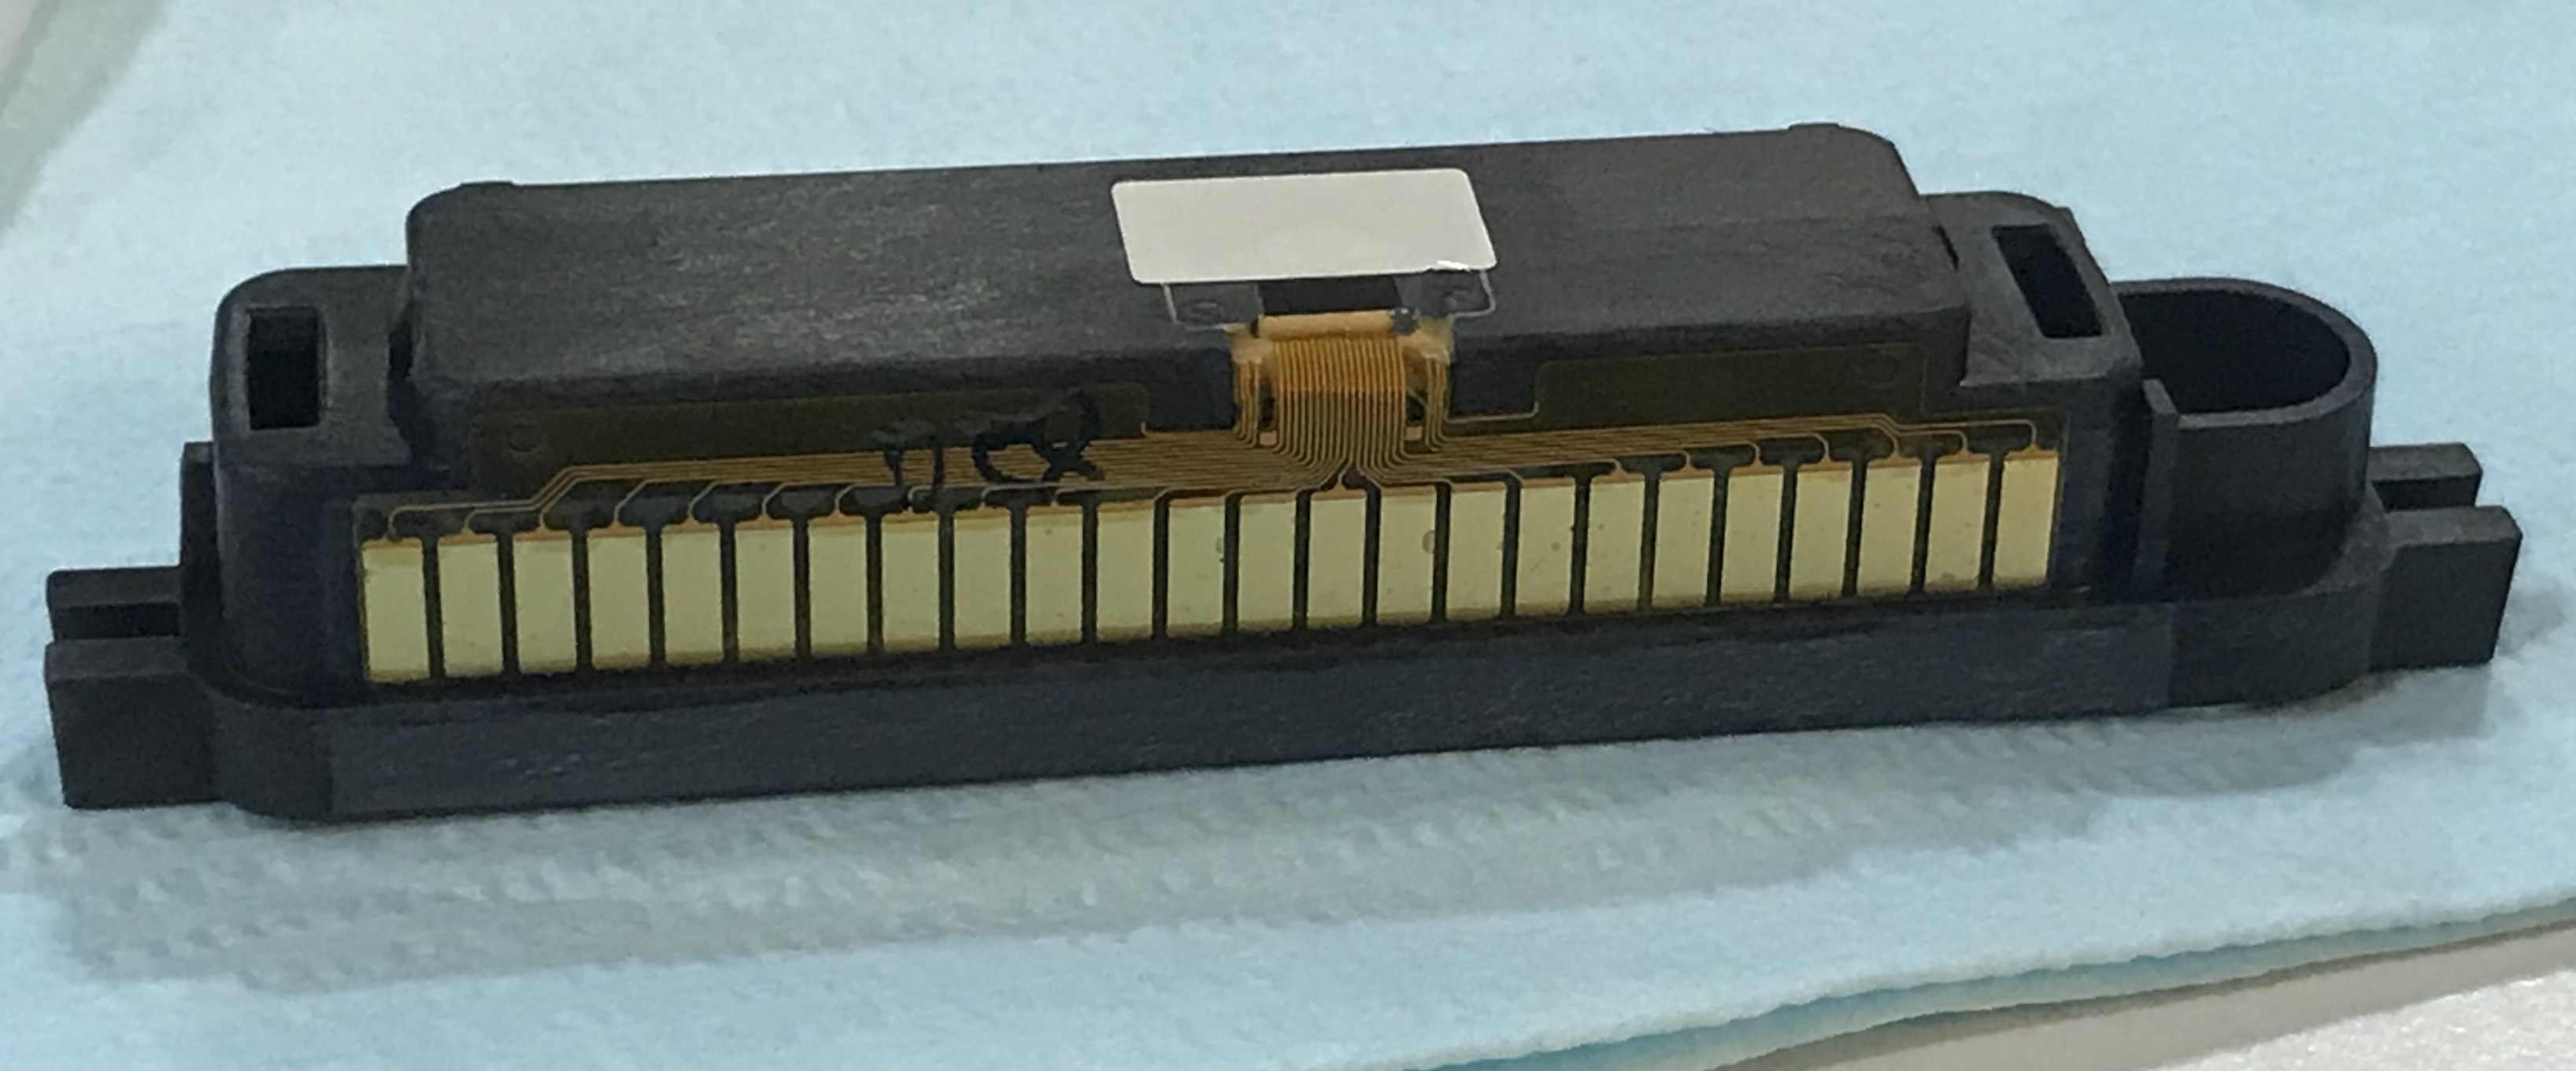
\includegraphics[width=0.5\textwidth]{Figuras/Figura_cabezal}
  \caption{Cabezal de impresora Fujifilm Dimatix DMP-2850.}
  \label{fig:Figura_cabezal}
\end{figure}

El correspondiente a la impresora Fujifilm Dimatix DMP2850 posee 16 eyectores, con los que se puede realizar distintas combinaciones, logrando diferentes espaciados entre gotas y por ende, distintos anchos de líneas. El cartucho completo consta del cabezal y un reservorio de 3 ml, que puede ser llenado con tintas de diferentes materiales (Figura ~\ref{fig:Figura_cartucho_completo}).

\begin{figure}[H]
  \centering
    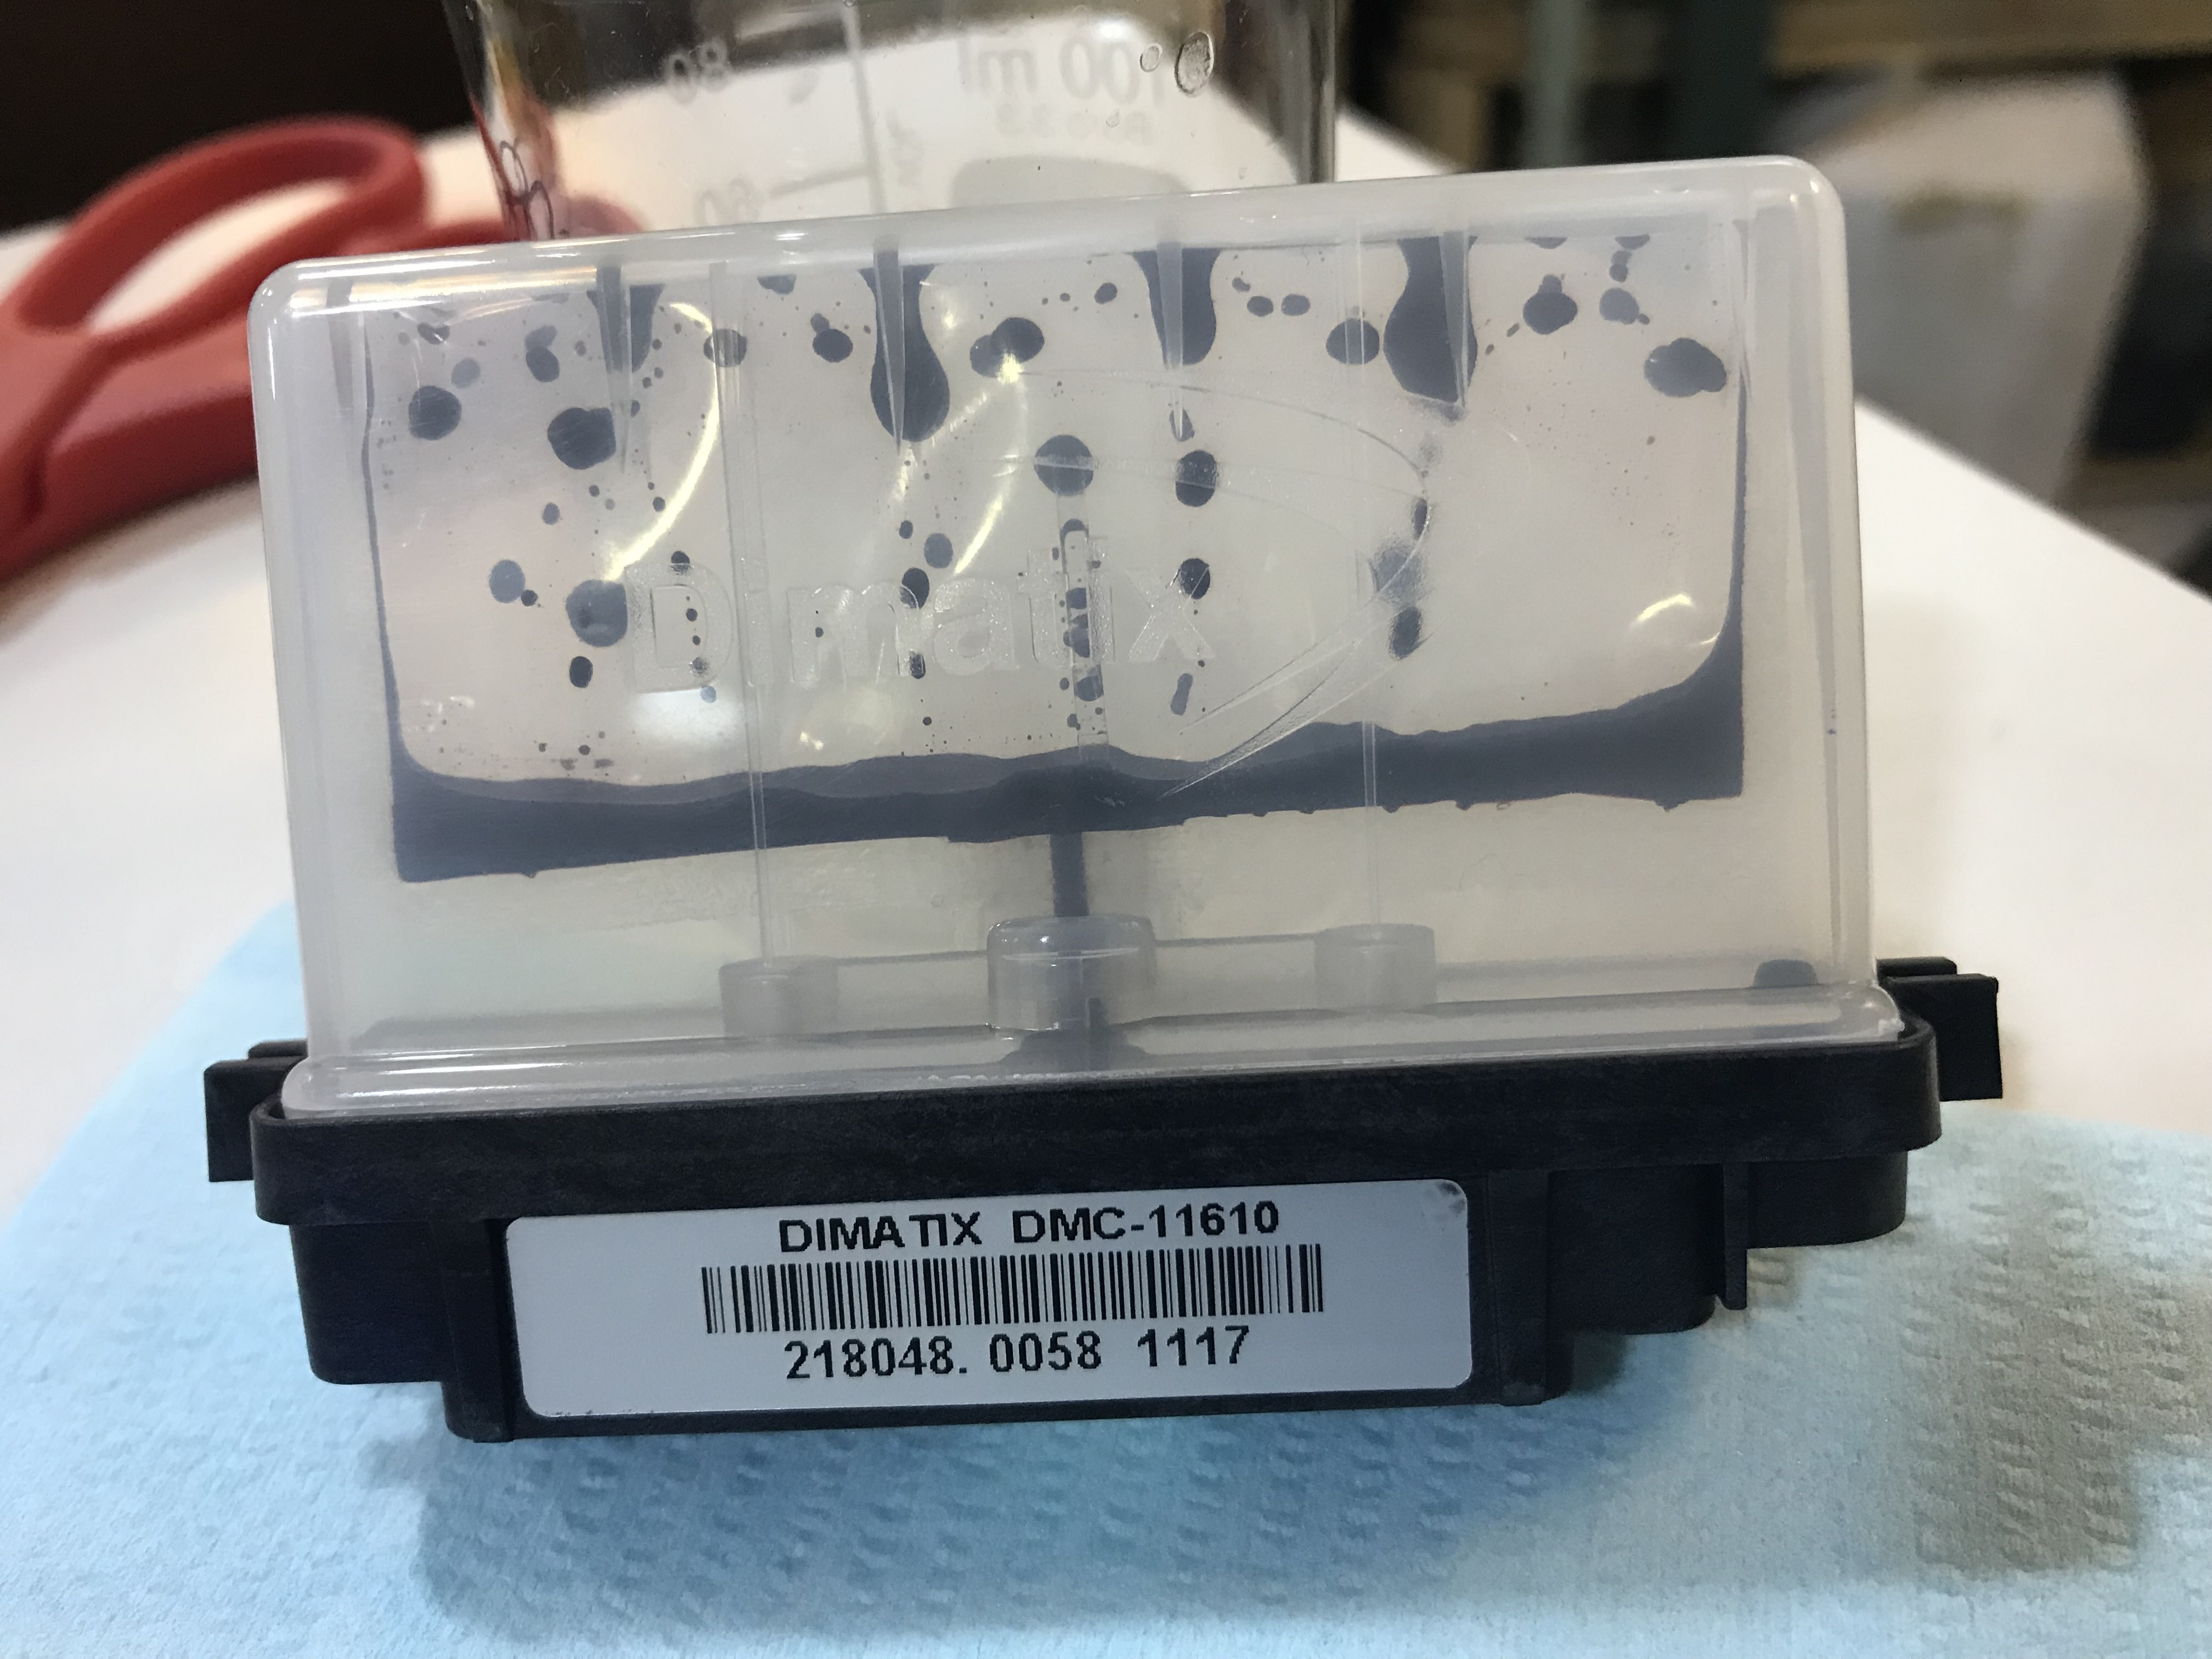
\includegraphics[width=0.5\textwidth]{Figuras/Figura_cartucho_completo}
  \caption{Cartucho de impresora Fujifilm Dimatix DMP-2850.}
  \label{fig:Figura_cartucho_completo}
\end{figure}

Como ejemplos, Fujifilm informa que puede imprimirse gráfica, electrónica, \textit{displays}, químicos, objetos ópticos, objetos fotovoltáicos, objetos mecánicos en 3D y elementos de la ciencia de la vida como cadenas de ADN.

\subsection{Tinta de nanopartículas de oro}
En este proyecto se utilizará una tinta con nanopartículas de oro, fabricada por \textit{C-INK Company} bajo el nombre comercial de \textit{Drycure Au-JB 1010B} \cite{DrycureAu}. Esta tinta contiene partículas nanométricas de oro (Au). Si bien no está comprobado el efecto de las mismas en el cuerpo humano, debe tenerse extrema precaución al manipularla. Por esto, el fabricante recomienda utilizarla en un ambiente con buena ventilación o sistema de extracción, utilizar protección respiratoria en caso de presentarse vapores. En todo momento deben usarse guantes, anteojos y ropa de trabajo, sobretodo al momento de manipular la tinta.

Dentro de su composición se tiene, dado como porcentaje en peso, 9-11 \% de Oro, 36-40 \% de agua, 48-52 \% de Glycerol, 0.1-1.0 \% de Alcohol, 0.1-0.5 \% de \textit{Acetylene glycol} y 0.1-2.0 \% de resina Polyester.

Como caracteristicas físicas y químicas, se indica que la tinta es liquida, es una solución miscible, tiene una densidad de 1.10 a 1.20 g/ml y una viscosidad de 9 a 11 mPa$\cdot$s.

Dado que la tinta está formulada a base de agua, debe mantenerse a bajas temperaturas y sellada hermeticamente para evitar la evaporación del solvente o la excesiva humedad, que pueden provocar cambios en sus características (Figura ~\ref{fig:Figura_tinta_Au}).

\begin{figure}[H]
  \centering
    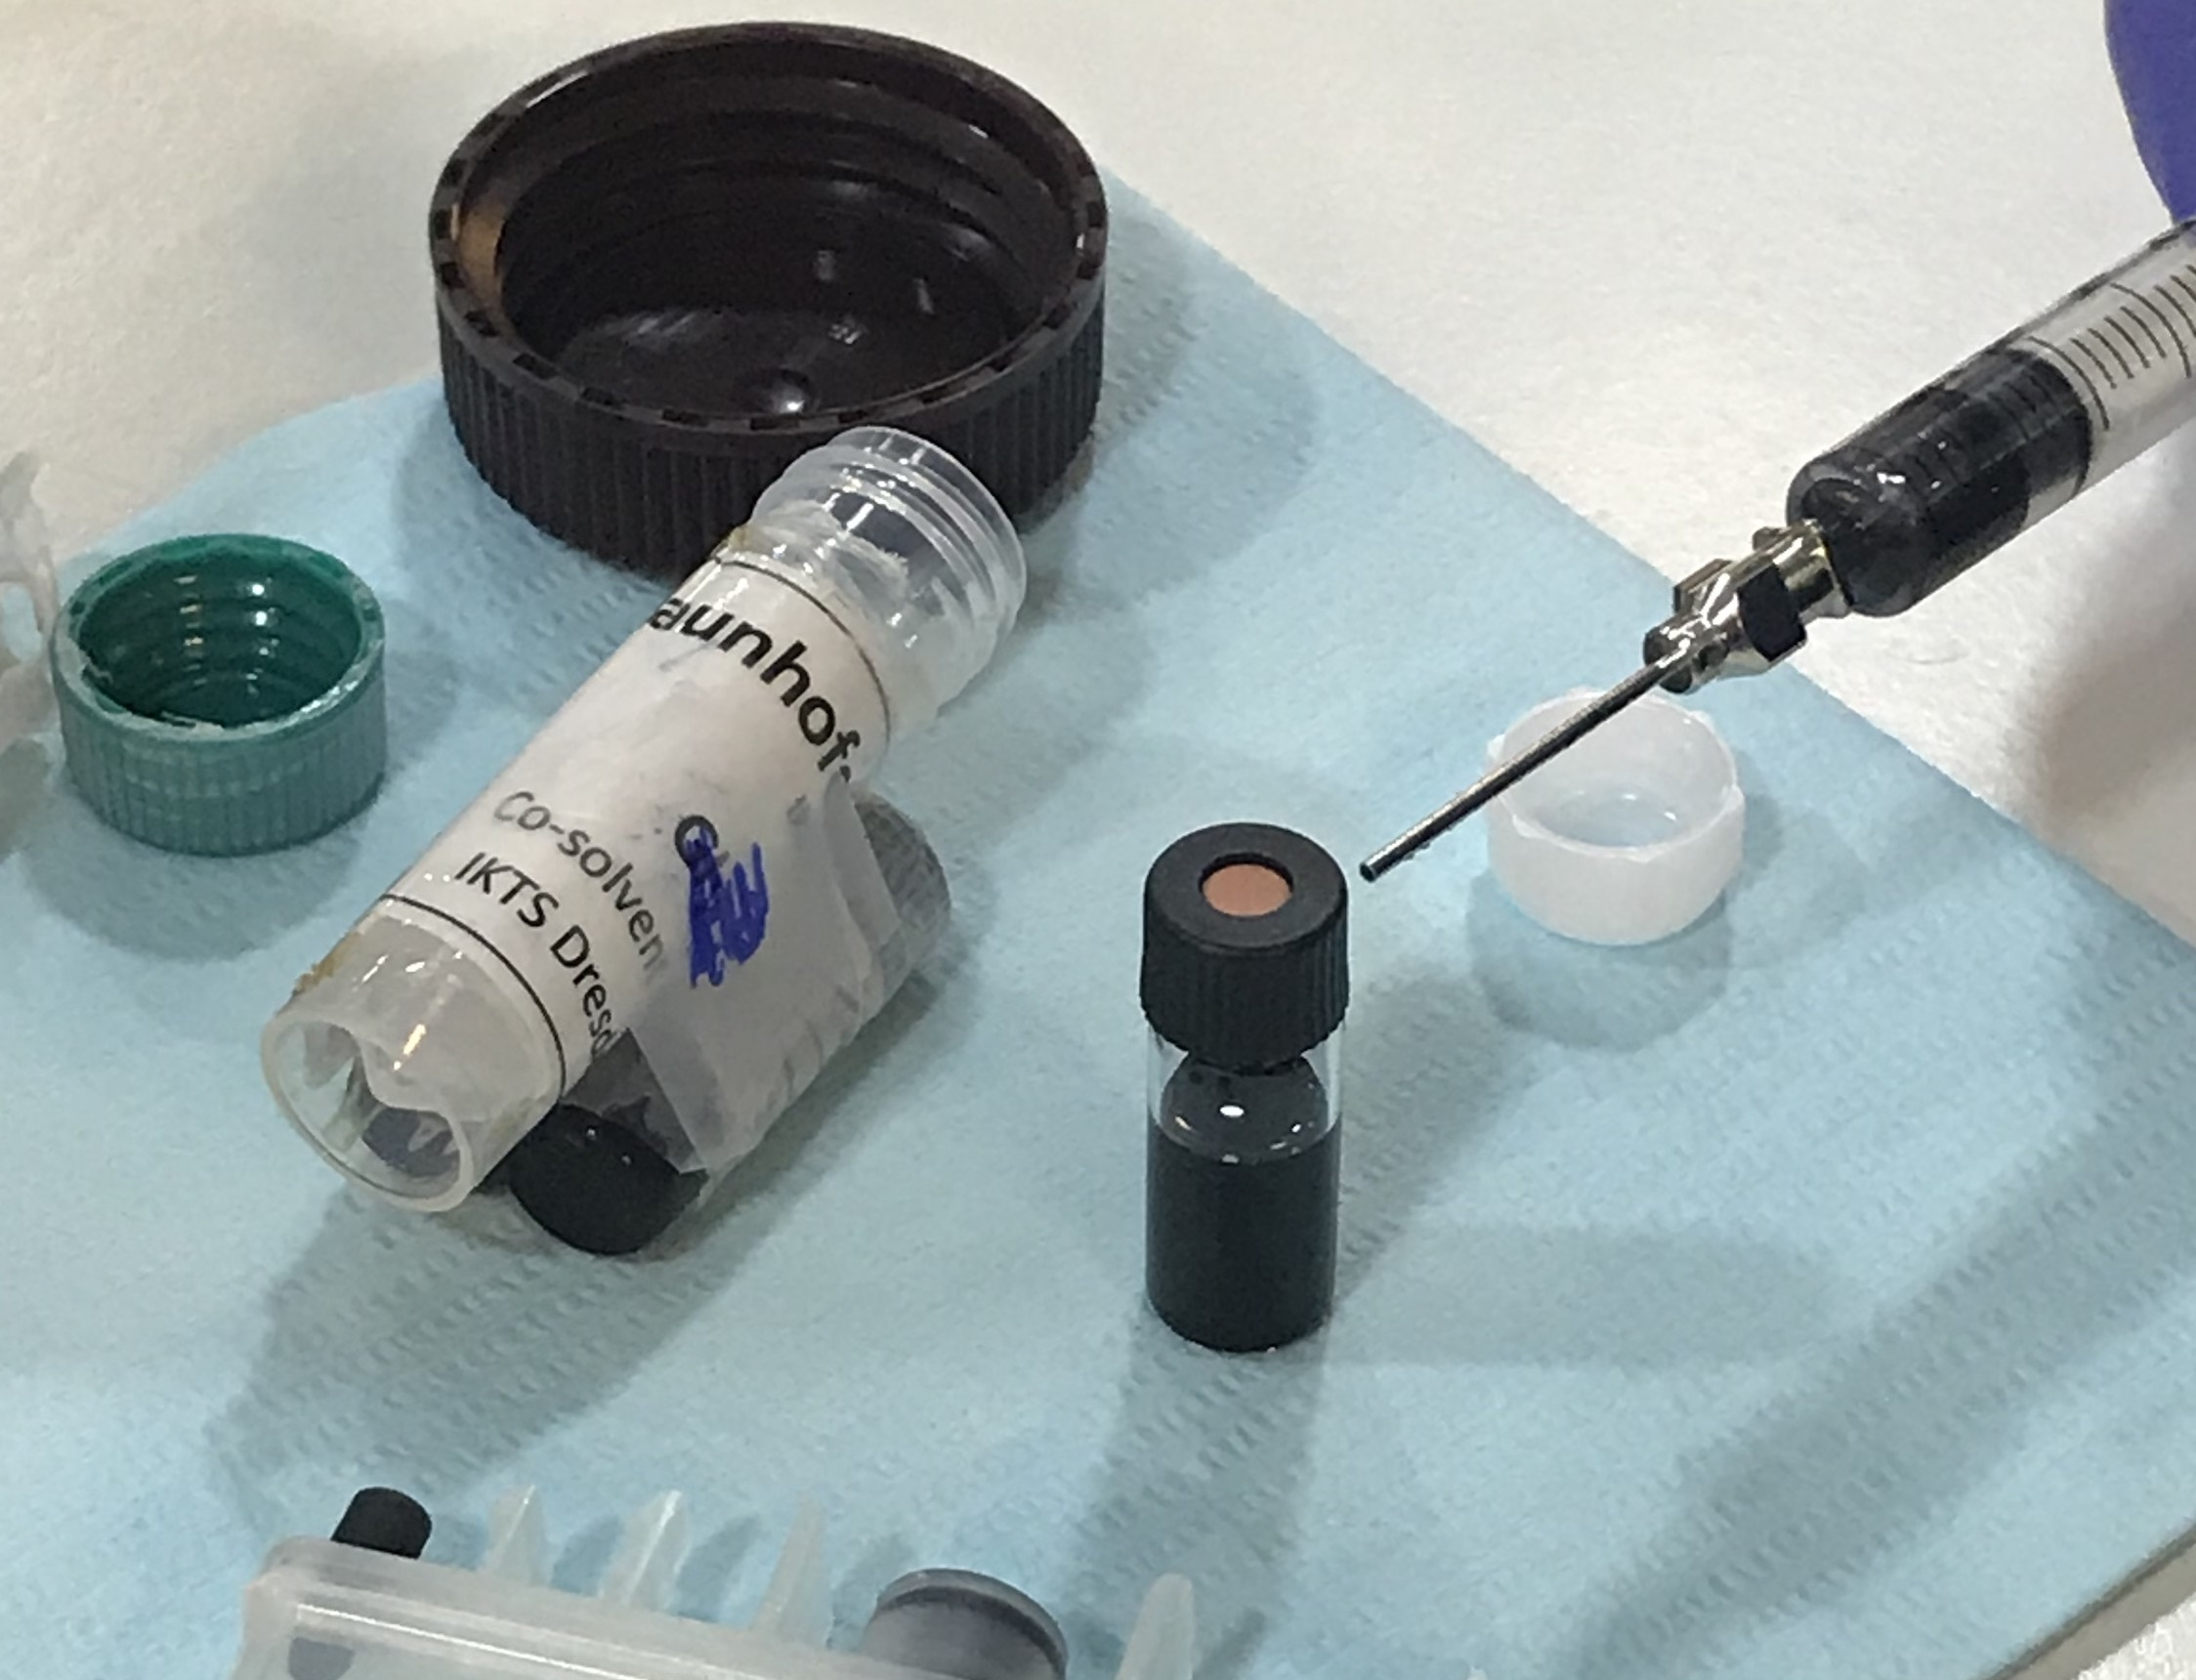
\includegraphics[width=0.5\textwidth]{Figuras/Figura_tinta_Au}
  \caption{Recipiente con tinta de nanopartículas de oro sellado herméticamente.}
  \label{fig:Figura_tinta_Au}
\end{figure}

\subsection{Tinta dieléctrica fotodefinible SU-8}
La tinta dieléctrica usada en este proyecto es \emph{PriElex SU-8 2007} de la firma \emph{MicroChem}. La misma se basa en el compuesto SU-8, es compatible con procesos de impresión por \textit{Inkjet} y puede curarse térmicamente sin la necesidad de exposición a rayos UV. (Figura ~\ref{fig:Figura_tinta_SU8}).

Algunas de sus ventajas más destacadas son su baja temperatura de curado ($<$ 150ºC), excelente estabilidad térmica y alta resistencia química.

Posee una tensión superficial de 30 dinas/cm, una densidad de 1,038 g/cm\textsuperscript{3} y una viscosidad cinemática de 9,33 cSt. Estas propiedades se encuentran informadas en la hoja de datos del fabricante \cite{PriElexSU8}.

\begin{figure}[H]
  \centering
    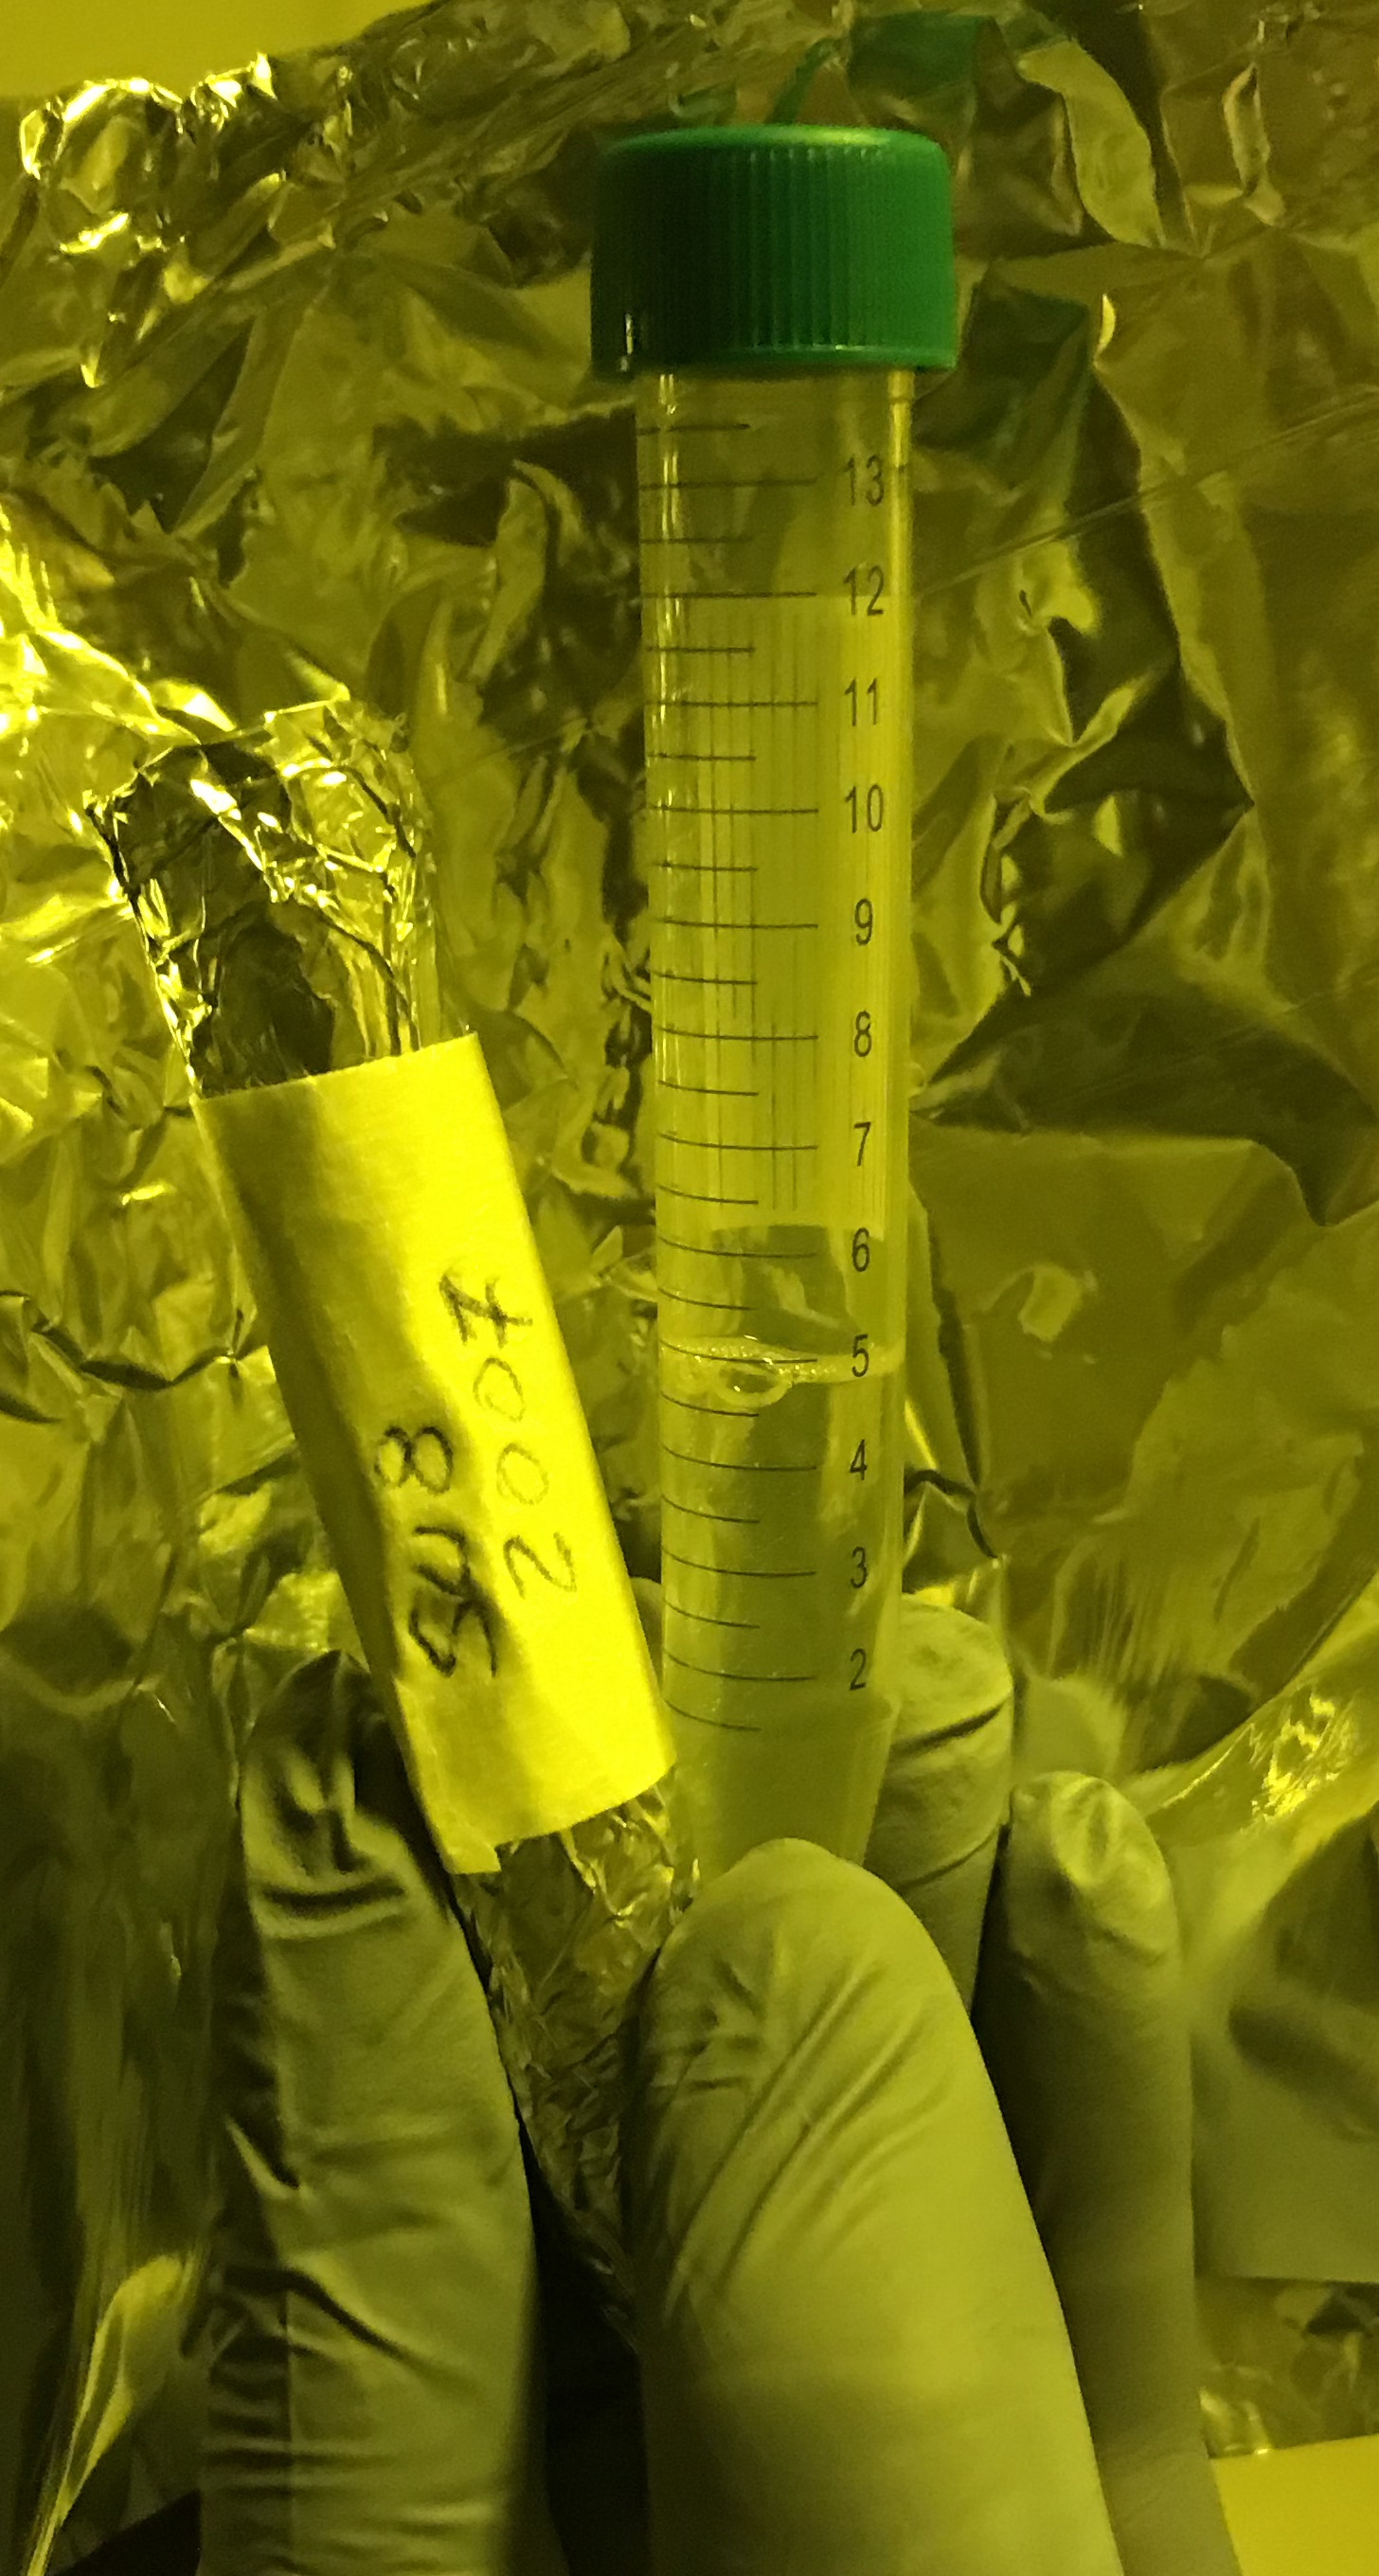
\includegraphics[width=0.2\textwidth]{Figuras/Figura_tinta_SU8}
  \caption{Recipiente con tinta dieléctrica SU-8.}
  \label{fig:Figura_tinta_SU8}
\end{figure}

\subsection{Sustrato \textit{Valox}}
El sustrato, donde se imprimirán los biosensores, es una película de tereftalita y polibutileno termoplástico. El mismo se comercializa en diferentes espesores, para este proyecto se utilizó el de 600 $\mu$m (Figura ~\ref{fig:Figura_Valox}).

Este compuesto posee una excelente resistencia dieléctrica y una fácil manipulación para realizar termoformados, estampados y doblados, lo que lo hace adecuado para una amplia gama de aplicaciones eléctricas, electrónicas y médicas \cite{Valox}.

\begin{figure}[H]
  \centering
    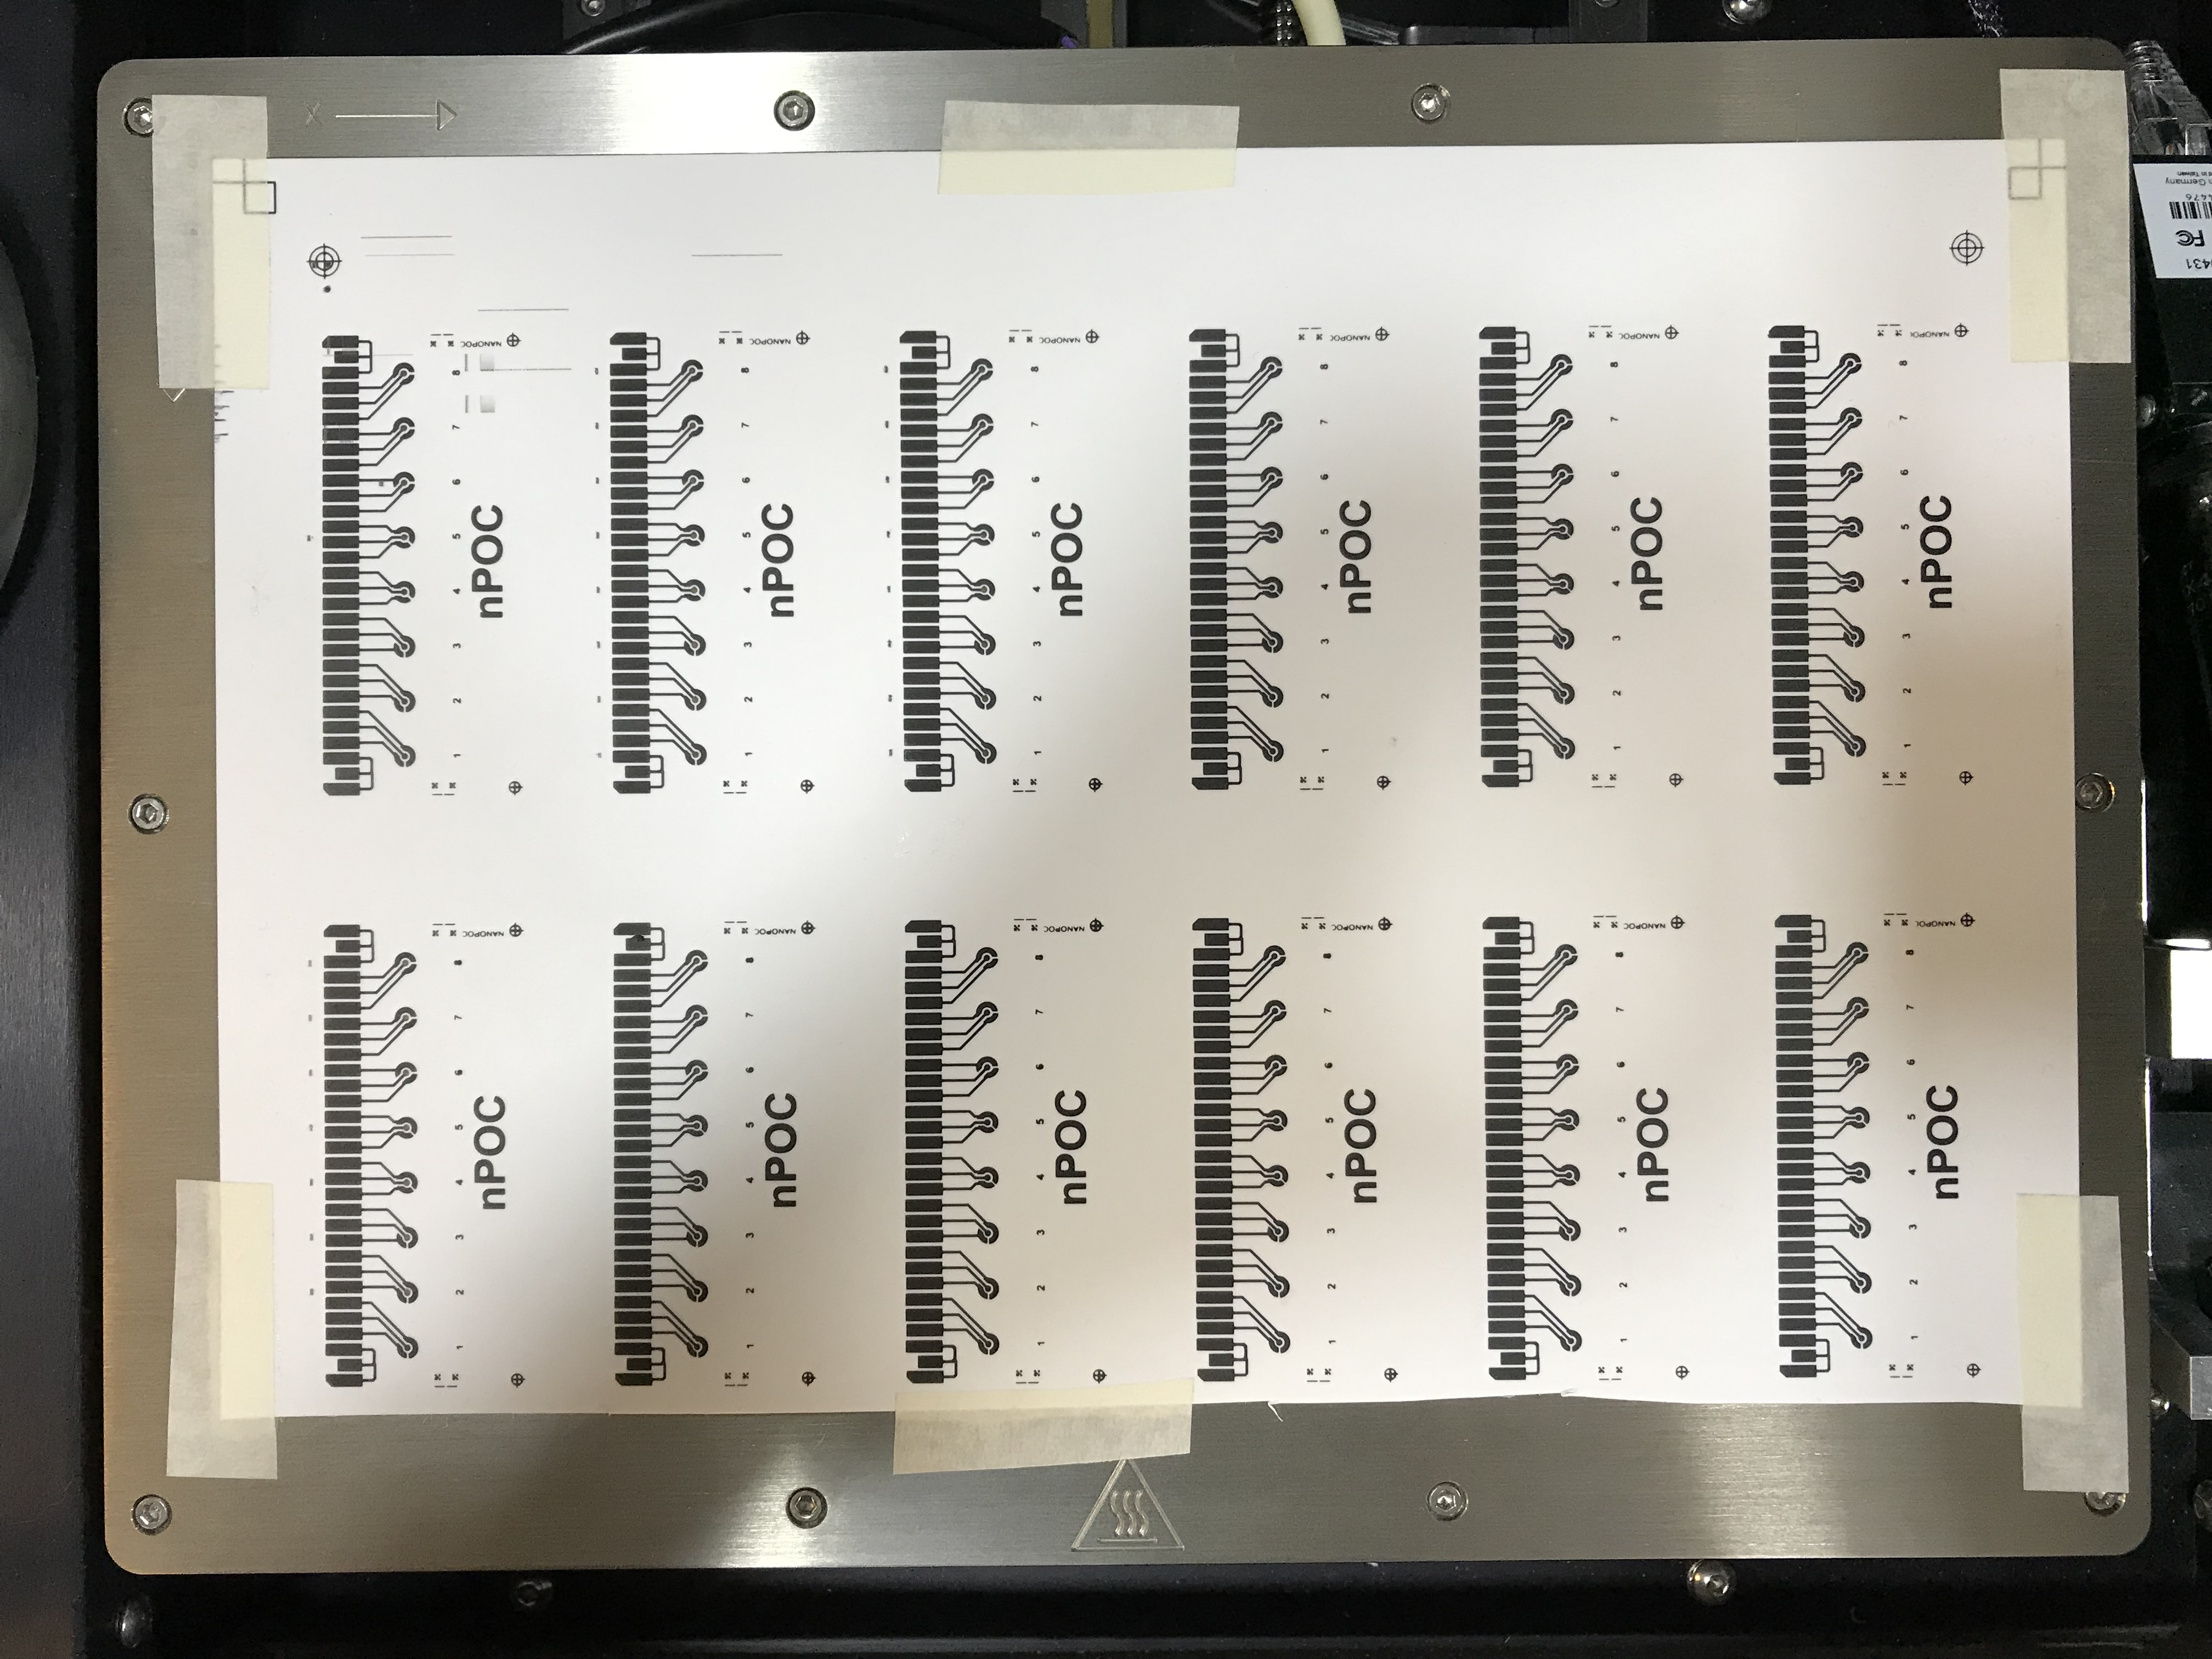
\includegraphics[width=0.55\textwidth]{Figuras/Figura_Valox}
  \caption{Sustrato \textit{Valox} con impresión serigráfica de carbono.}
  \label{fig:Figura_Valox}
\end{figure}

\section{T\'ecnicas de Caracterizaci\'on}
\subsection{Caracterizaci\'on El\'ectrica}\label{subsec:carac_elec}
Debido a la escala en que se imprime la tinta de nanopartículas puede presentar microfisuras invisibles a la vista e imágenes de poco aumento, sin embargo, son perceptibles en imágenes aumentadas por microscopio (Figura ~\ref{fig:Figura_Carac_elec}).

\begin{figure}[H]
  \centering
    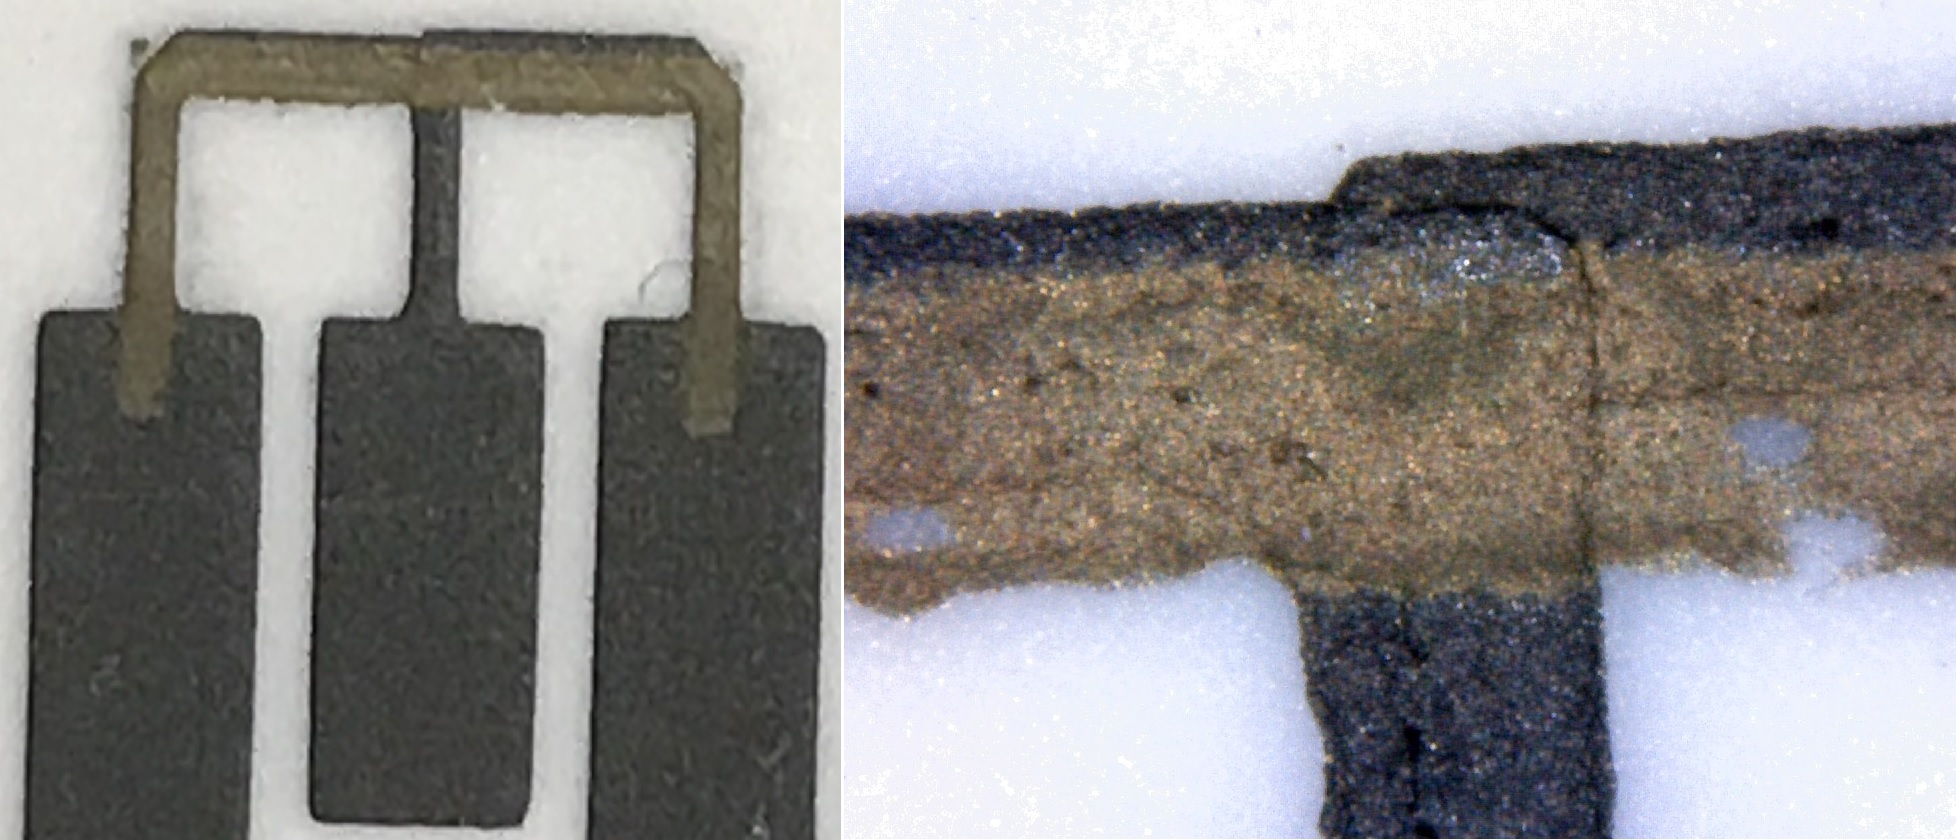
\includegraphics[width=0.5\textwidth]{Figuras/Figura_Carac_elec}
  \caption{Imagen con cámara convencional (iPhone 7) e imagen con microscopio USB Aumento 1000X.}
  \label{fig:Figura_Carac_elec}
\end{figure}

A través de una medición de resistencia a 4 puntas (conocido como método de Kelvin), se puede asegurar la continuidad física de la película, el correcto funcionamiento de la impresora y por ende del eléctrodo de trabajo del biosensor.

El método utiliza dos circuitos vinculados por una fuente de corriente continua. Por uno circula la corriente proveniente de la fuente, medida por un amperimetro y el otro posee un voltímetro en paralelo con la resistencia a medir. También se encuentra el sistema dual al anterior, dónde se tiene una fuente de tensión verificada con un voltímetro y un amperímetro que mide la corriente circulante por la resistencia (Figura ~\ref{fig:Figura_metodo_Kelvin}).

\begin{figure}[H]
  \centering
    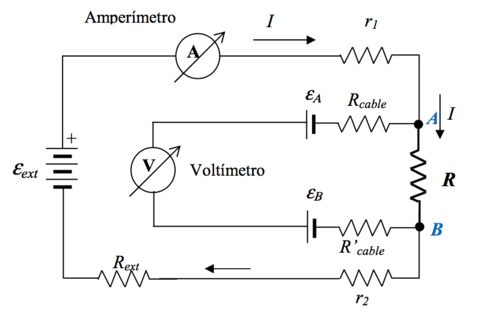
\includegraphics[width=0.5\textwidth]{Figuras/Figura_metodo_Kelvin}
  \caption{Circuito de medición a cuatro puntas.}
  \label{fig:Figura_metodo_Kelvin}
\end{figure}


\subsection{Caracterizaci\'on \'Optica/Dimensional}
Como parte de una caracterización óptica o dimensional es importante saber tamaños, espesores y rugosidades.

Los tamaños pueden obtenerse a través de la cámara fiducial de la impresora. El software de la misma permite realizar mediciones de distancias entre dos puntos y de esta forma obtener todos los valores requeridos en la caracterización (Figura ~\ref{fig:Figura_Cam_Fiducial_Medicion}).

\begin{figure}[H]
  \centering
    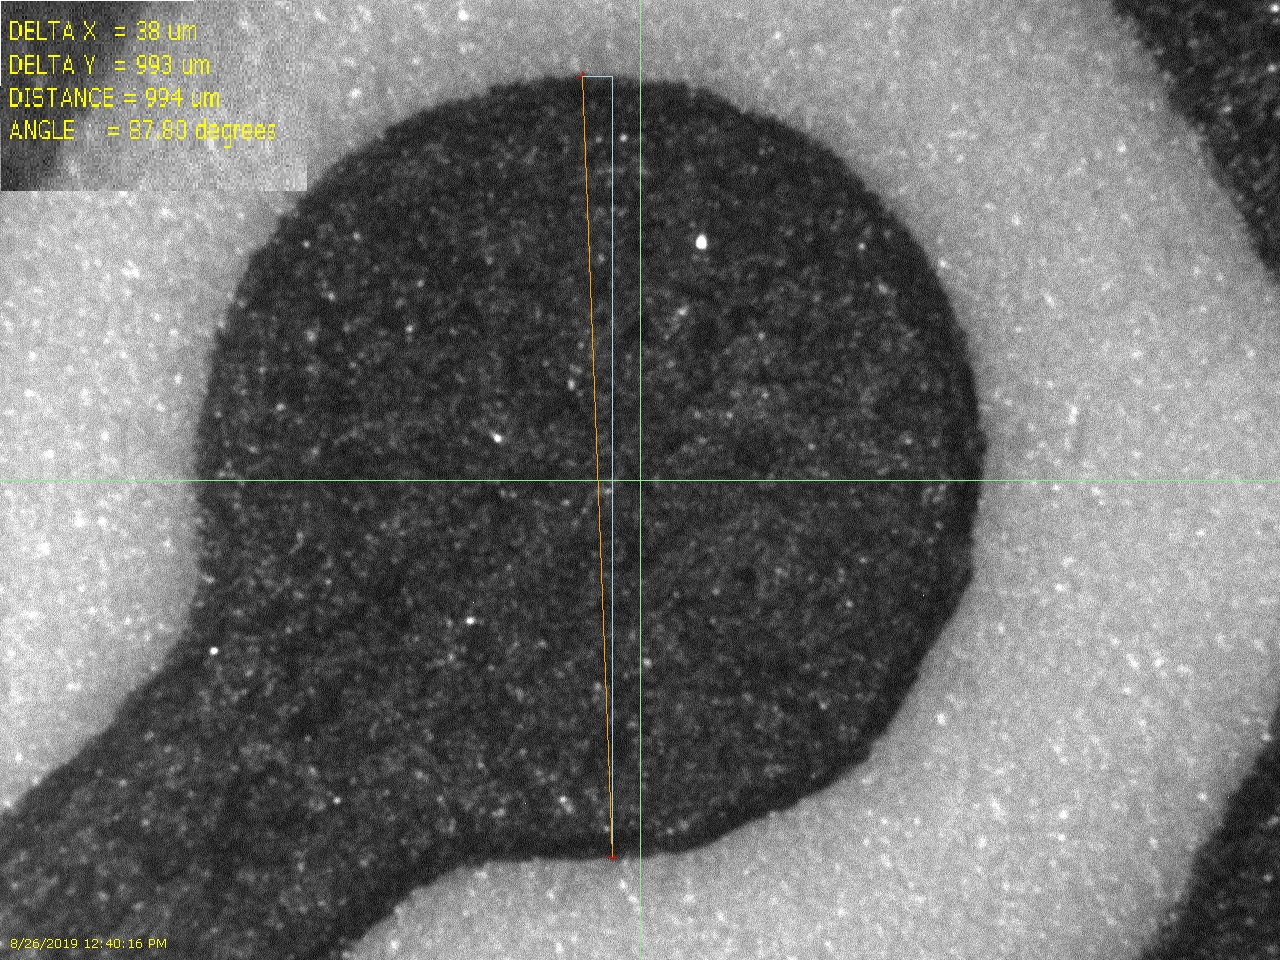
\includegraphics[width=0.5\textwidth]{Figuras/Figura_Cam_Fiducial_Medicion}
  \caption{Imagen de cámara fiducial con medición de distancias.}
  \label{fig:Figura_Cam_Fiducial_Medicion}
\end{figure}

A través de un perfilómetro de contacto se puede obtener el espesor de las impresiones y la rugosidad de las superficies. Este equipo, también llamado rugosímetro, utiliza una punta fina en contacto con la superficie a analizar (Figura ~\ref{fig:Figura_Stylus}), realizando un barrido controlado en línea recta. Las variaciones de alturas detectadas por esta punta son convertidas en señales eléctricas y pueden ser registradas o graficadas.

\begin{figure}[H]
  \centering
    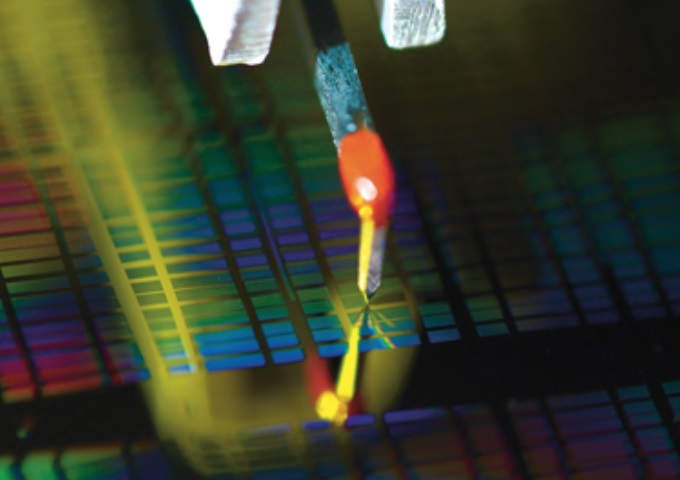
\includegraphics[width=0.5\textwidth]{Figuras/Figura_Stylus}
  \caption{Imagen de punta tipo Stylus de un perfilómetro de contacto.}
  \label{fig:Figura_Stylus}
\end{figure}

La rugosidad es un dato importante en la caracterización, ya que esta define el área efectiva de funcionamiento del biosensor. Cuanto más lisa sea la superficie, el área efectiva se aproximará al área geométrica del electrodo.

\subsection{Caracterizaci\'on Electroqu\'imica}
Para este trabajo se utiliza el procedimiento de voltametría cíclica de corriente continua. Esta caracterización electroquímica consiste en variar, de manera cíclica, el potencial del electrodo de trabajo respecto de uno de referencia. Ambos se sumergen en una solución y se mide la corriente resultante que circula por el electrodo de trabajo (Figura ~\ref{fig:Figura_circuito_voltametria}). 
\begin{figure}[H]
  \centering
    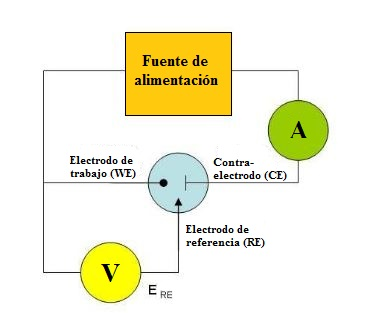
\includegraphics[width=0.65\textwidth]{Figuras/Figura_circuito_voltametria}
  \caption{Esquema de circuito eléctrico para voltametría cíclica de corriente contínua.}
  \label{fig:Figura_circuito_voltametria}
\end{figure}
La señal de excitación es un barrido de potencial lineal con una onda de forma triangular, la cual parte de un potencial E1, que evoluciona linealmente en el tiempo hasta un potencial E2 para luego volver a E1 (Figura ~\ref{fig:Figura_Carac_electroquimica}). Las velocidades de este barrido pueden variar desde menos de 1 mV/s hasta cientos de volts por segundo \cite{TesisGG}.

\begin{figure}[H]
  \centering
    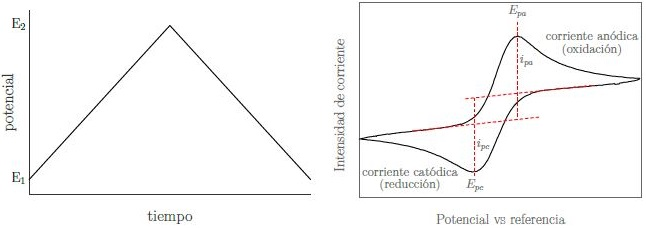
\includegraphics[width=1\textwidth]{Figuras/Figura_Carac_electroquimica}
  \caption{Curva de excitación y voltagrama típico para una especie redox reversible. Figura extraída de \cite{TesisGG}.}
  \label{fig:Figura_Carac_electroquimica}
\end{figure}

Se usaron como sondas electroquímicas ferrocianuro y ferricianuro. La elección de estas sondas se debe a la reversibilidad de los pares \textit{redox}, cuyas especies oxidada y reducida son económicas y fáciles de conseguir, solubles en solución acuosa y se comportan de forma cuasi reversible frente al intercambio electrónico.

Se espera, en la aproximación más simple, que sigan el comportamiento voltamétrico descrito por Randles-Sevcik \ref{ecuacion3}, donde la corriente pico $(i_{p})$ es proporcional a la concentración (C), a la raíz cuadrada de la velocidad de barrido (\textit{v}) y al área (A). Los demás parámetros se consideran constantes.

\begin{equation}\label{ecuacion3}
i_{p}=0,4463nFAC(\frac{nFvD}{RT})^{1/2}\
\end{equation}



\chapter{Desarrollo Experimental}
Para el siguiente proyecto se utilizaron como base celdas electroquímicas impresas en carbono por el método de serigrafía sobre un sustrato Valox (Figura ~\ref{fig:Figura_Electrodos_nPOC}). Mediante una impresora marca Fujifilm modelo Dimatix DMP-2850 se realizó la deposición de la tinta de oro sobre el electrodo de trabajo. Se caracterizaron las propiedades eléctricas, dimensionales y electroquímicas de la misma para corroborar el correcto funcionamiento de los sensores.

\begin{figure}[H]
  \centering
    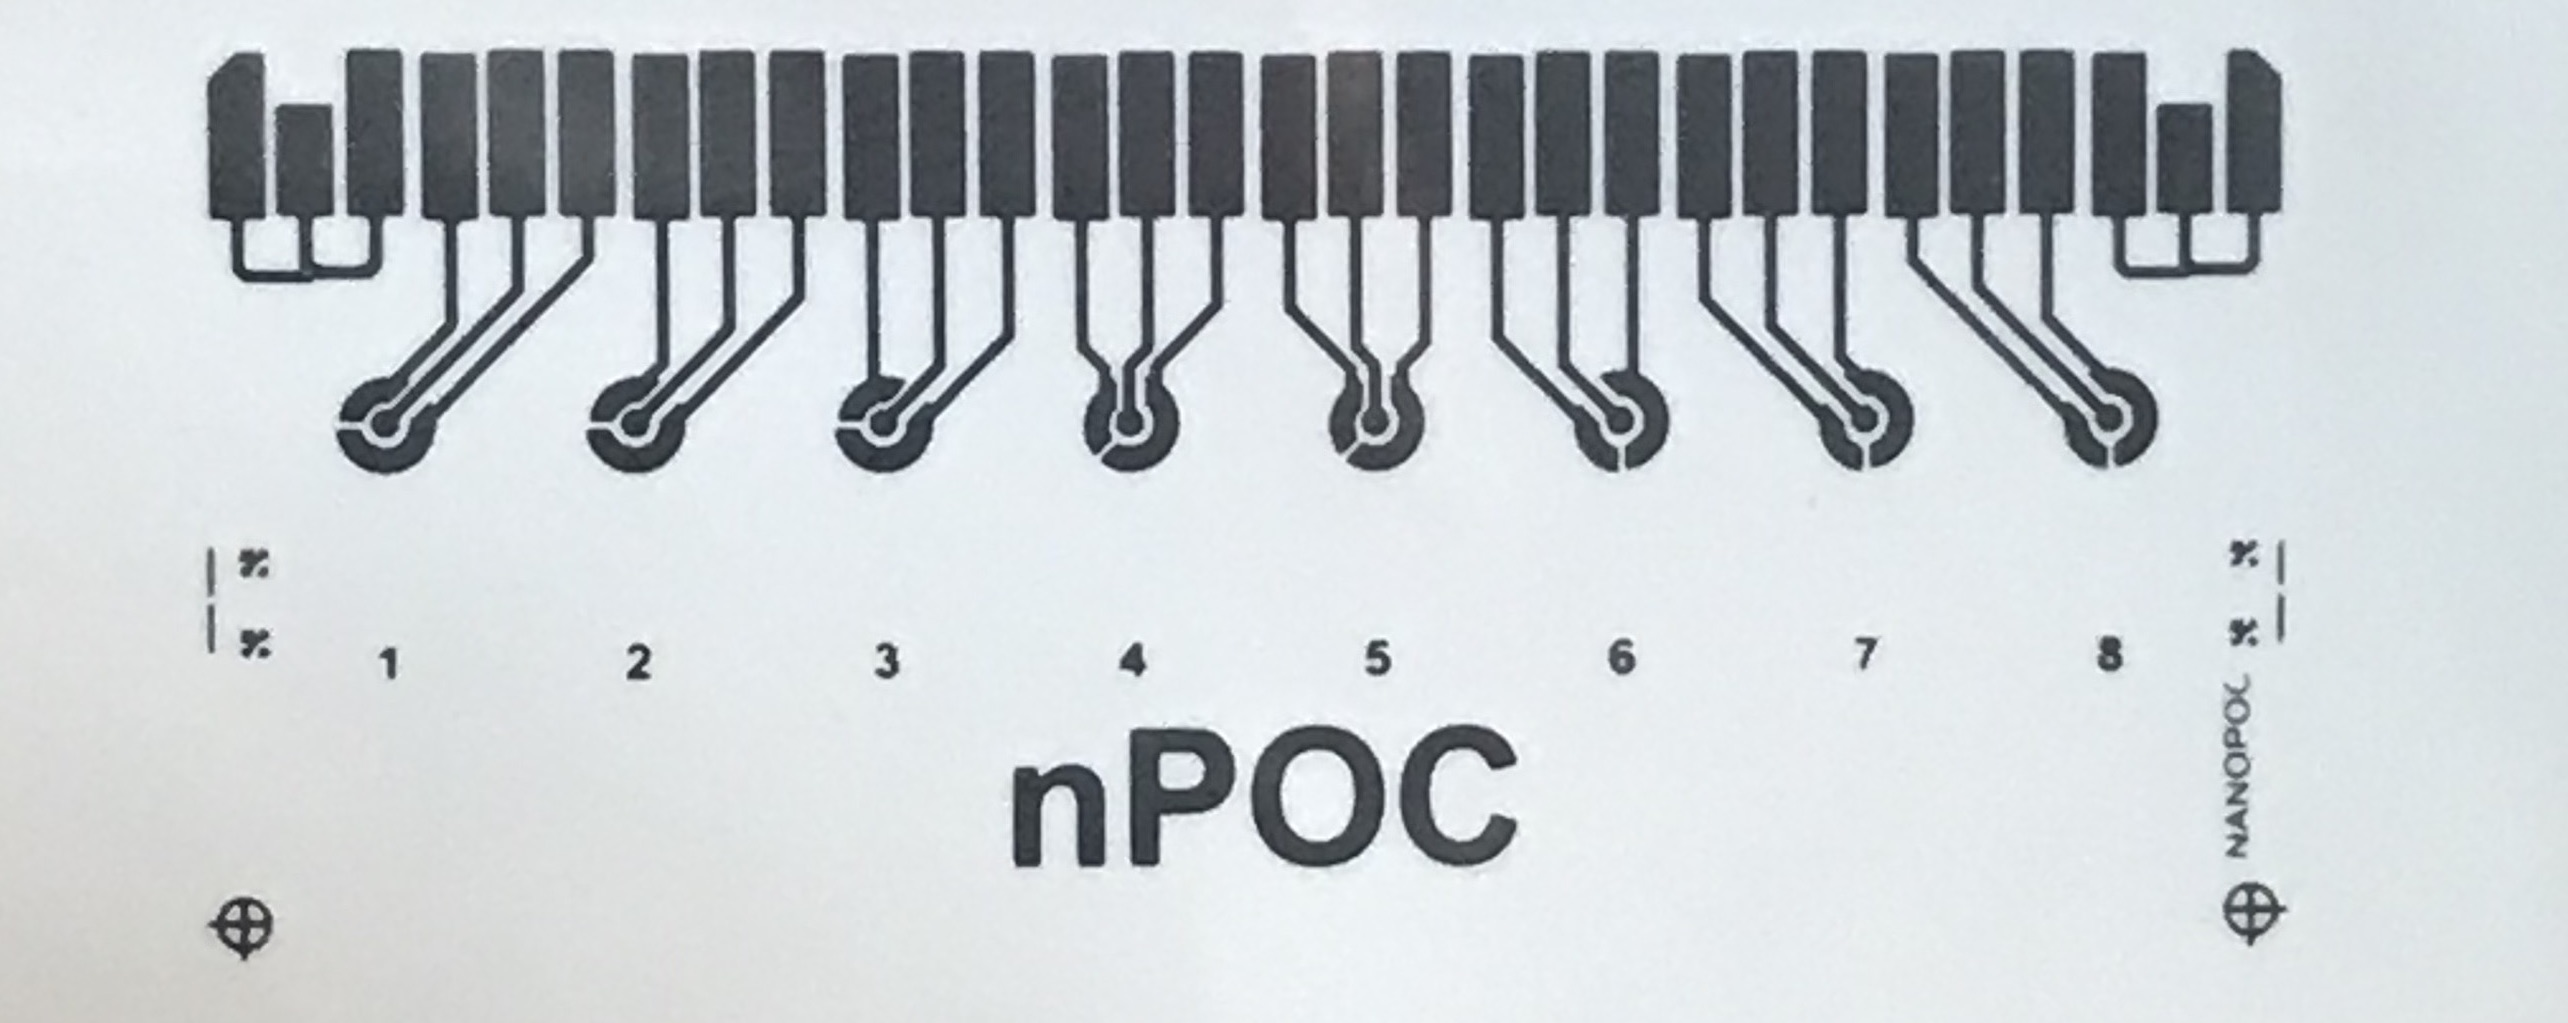
\includegraphics[width=0.5\textwidth]{Figuras/Figura_Electrodos_nPOC}
  \caption{Celdas Electroqu\'imicas}
  \label{fig:Figura_Electrodos_nPOC}
\end{figure}

\section{Preparación de patrones de imágenes}

\subsection{Mediciones previas}
Como primera instancia, se midieron los diferentes componentes de las celdas electroquímicas impresos en carbono. Se concluyó que los electrodos de trabajo (desde ahora \emph{WE}) poseen 1 mm de diámetro, donde se depositará la tinta de oro. La separación entre \emph{WE} y electrodo de referencia (desde ahora \emph{RE}) y contraelectrodo (desde ahora \emph{CE}) es de 400 $\mu$m. La distancia entre dos \emph{WE} es de 9 mm y cada cartucho cuenta con ocho sensores. Esta distancia medida entre dos \emph{WE} corresponde a la separación de una micro pipeta de ocho canales, utilizada en laboratorios. (Figura ~\ref{fig:Figura_medicion_celdas})

\begin{figure}[H]
  \centering
    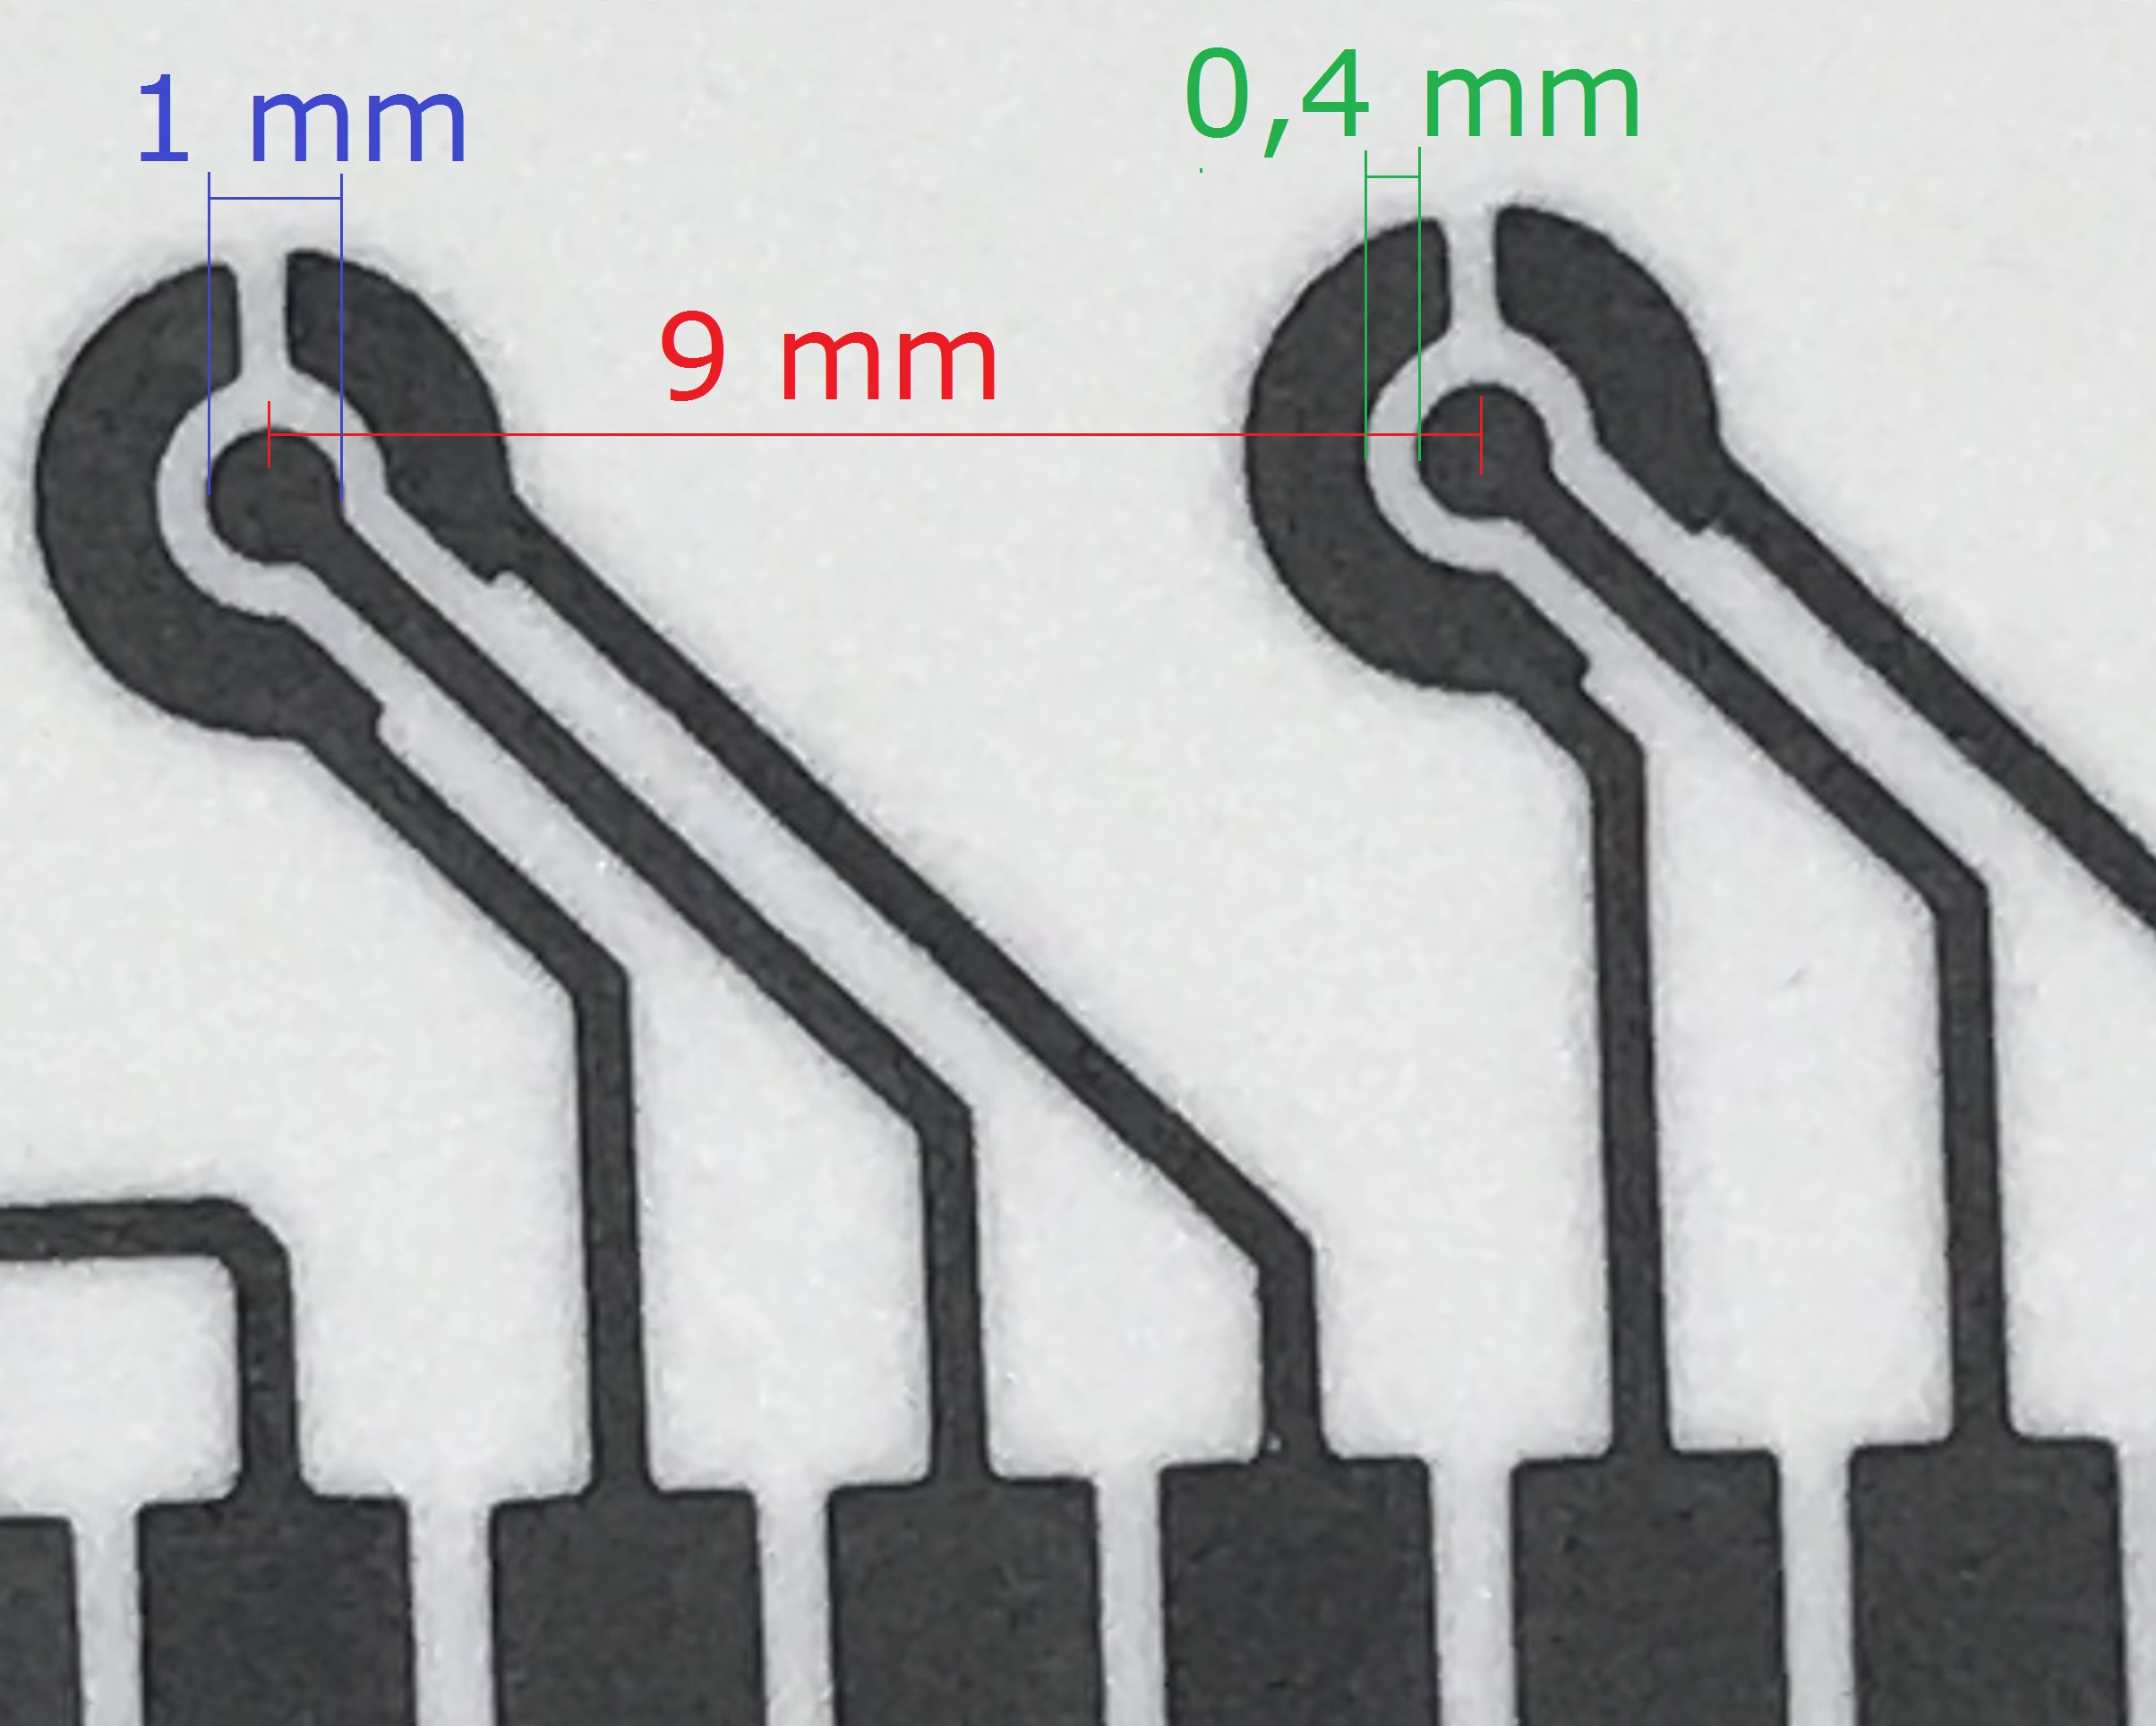
\includegraphics[width=0.5\textwidth]{Figuras/Figura_medicion_celdas}
  \caption{Mediciones dimensionales en sustrato.}
  \label{fig:Figura_medicion_celdas}
\end{figure}

Dado que las impresiones de carbono fueron realizadas por una empresa dedicada a impresiones serigráficas industriales, los biosensores se encuentran fabricados en dos columnas y seis filas dando un total de doce sensores por sustrato de tamaño A4 (Figura ~\ref{fig:Figura_sensores_hoja_A4}). Para tener un seguimiento preciso de los trabajos que se realizarán en cada muestra se los enumera aprovechando su nombre ya impreso en carbono como \textit{nPoc} del 1 al 5. (Figura ~\ref{fig:Figura_ejemplo_numeracion_nPoc})

\begin{figure}[H]
  \centering
    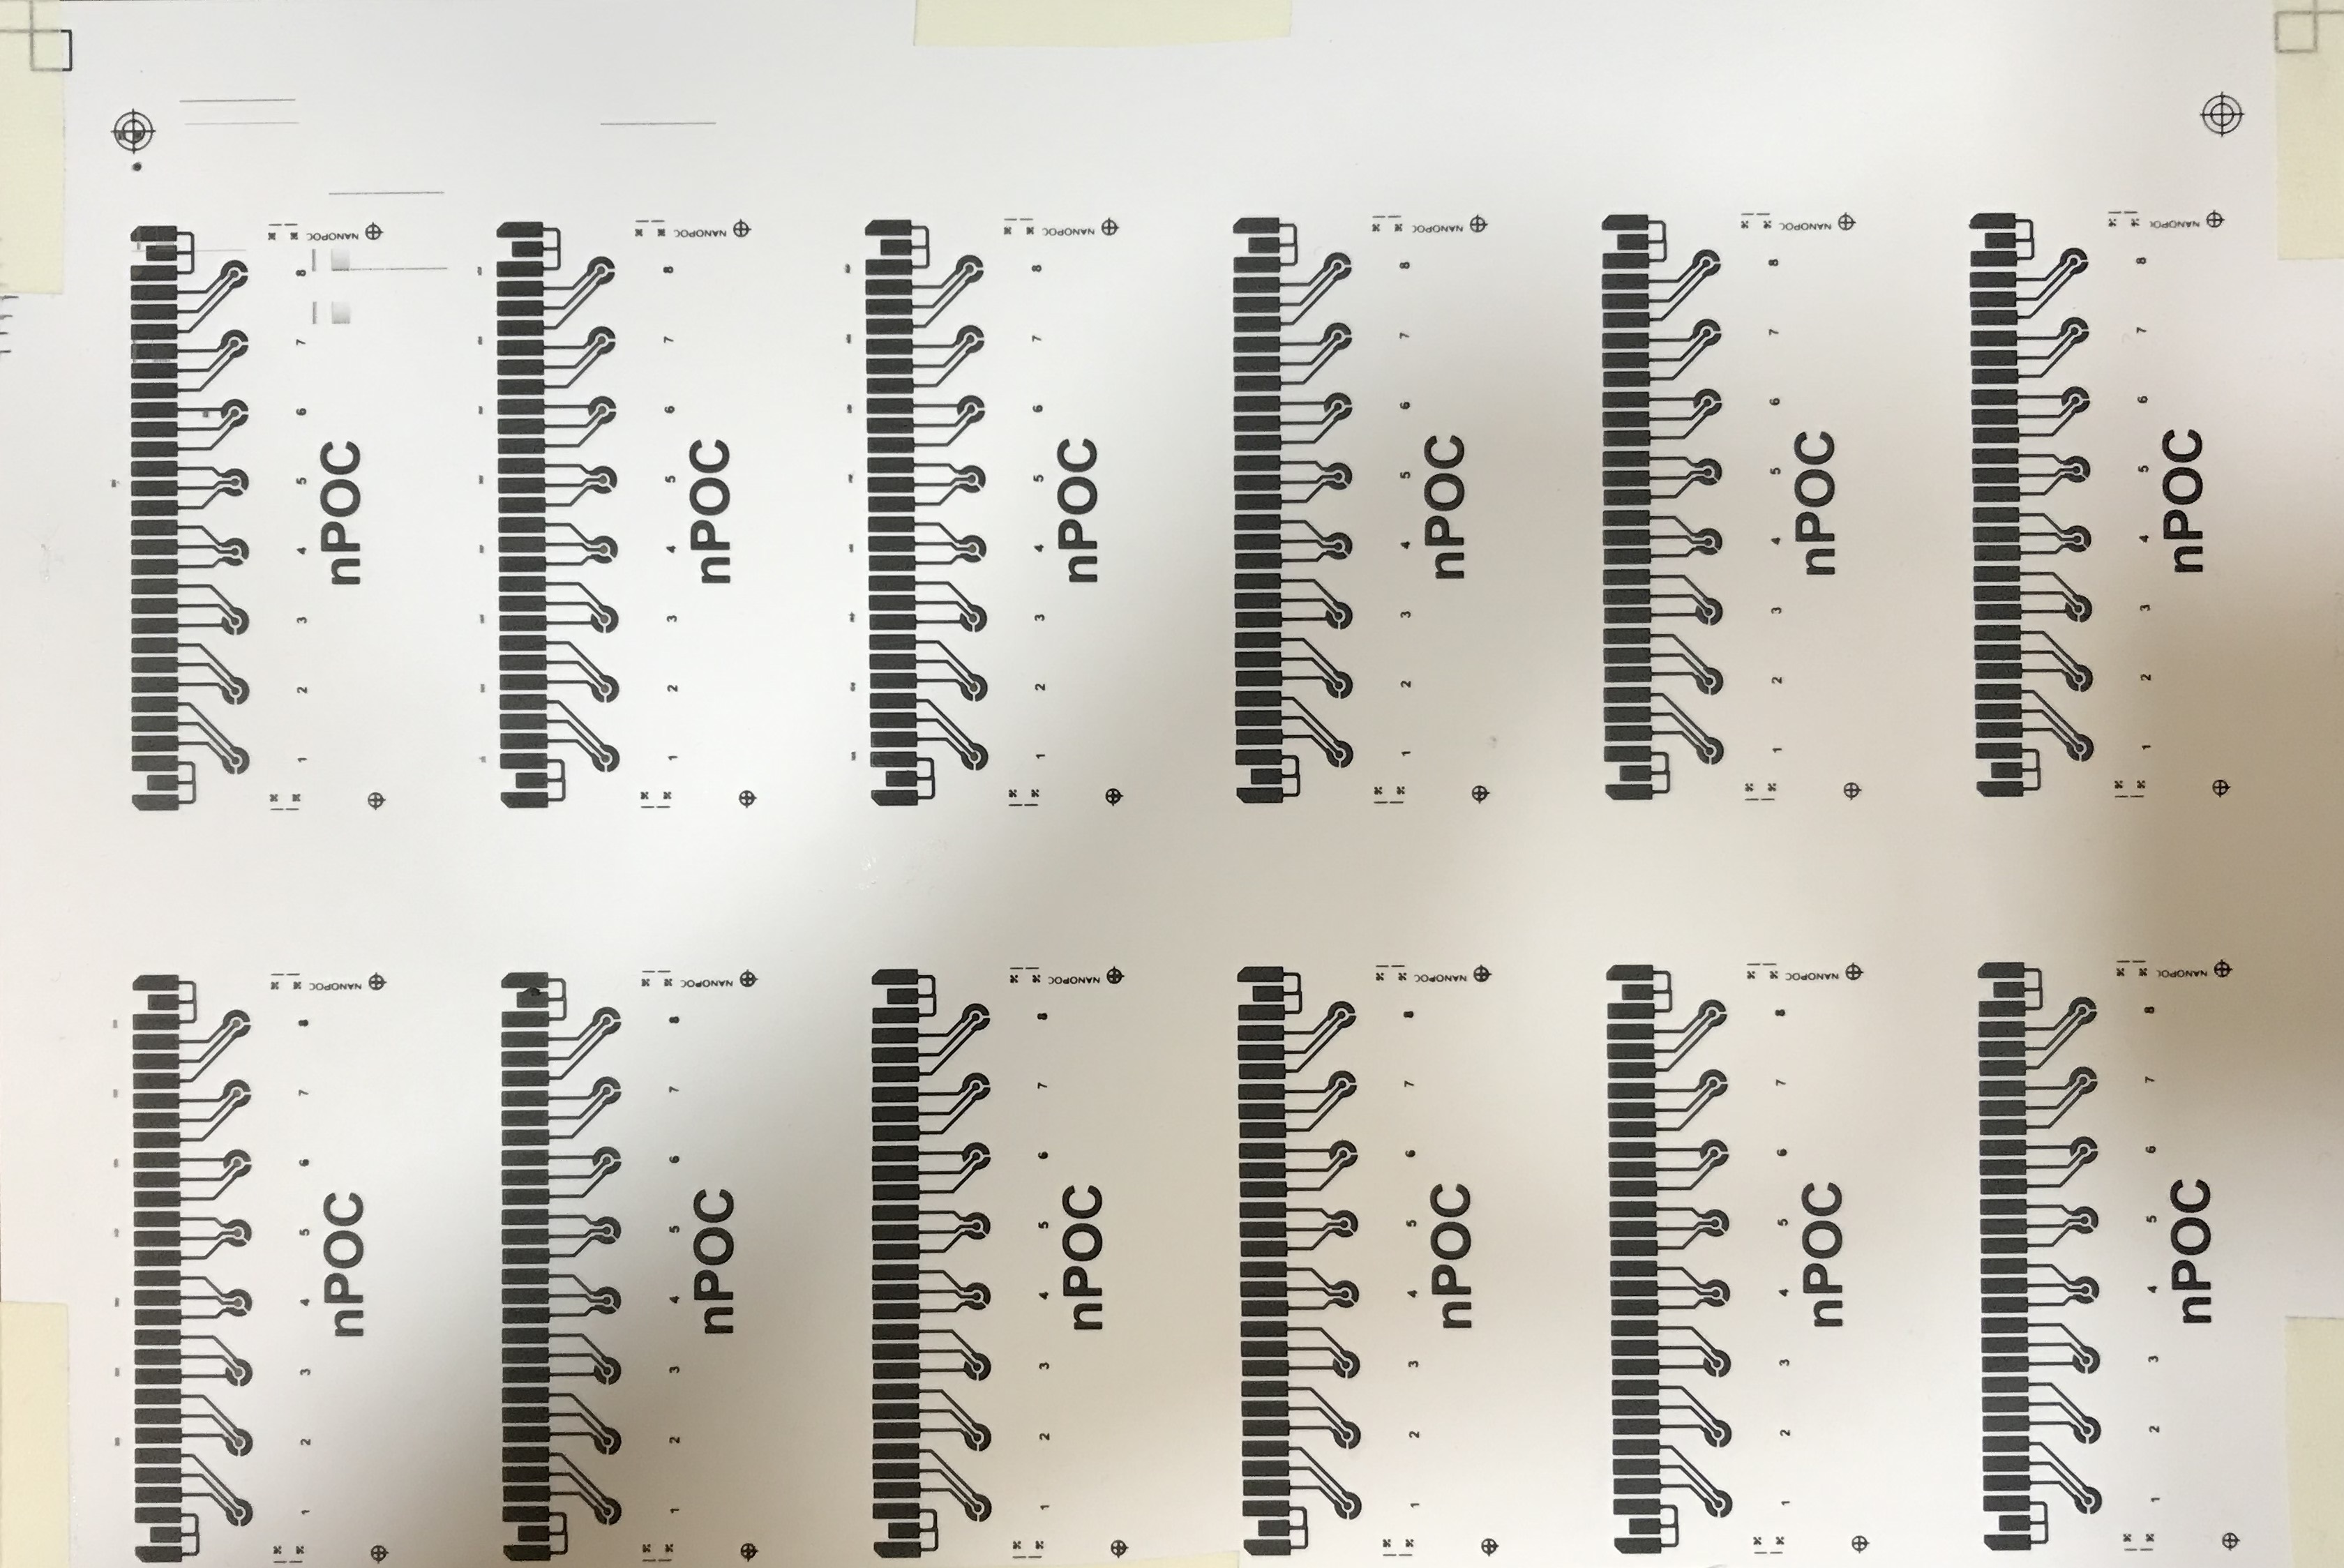
\includegraphics[width=0.5\textwidth]{Figuras/Figura_sensores_hoja_A4}
  \caption{Impresion serigráfica de biosensores en hoja A4}
  \label{fig:Figura_sensores_hoja_A4}
\end{figure}

\begin{figure}[H]
  \centering
    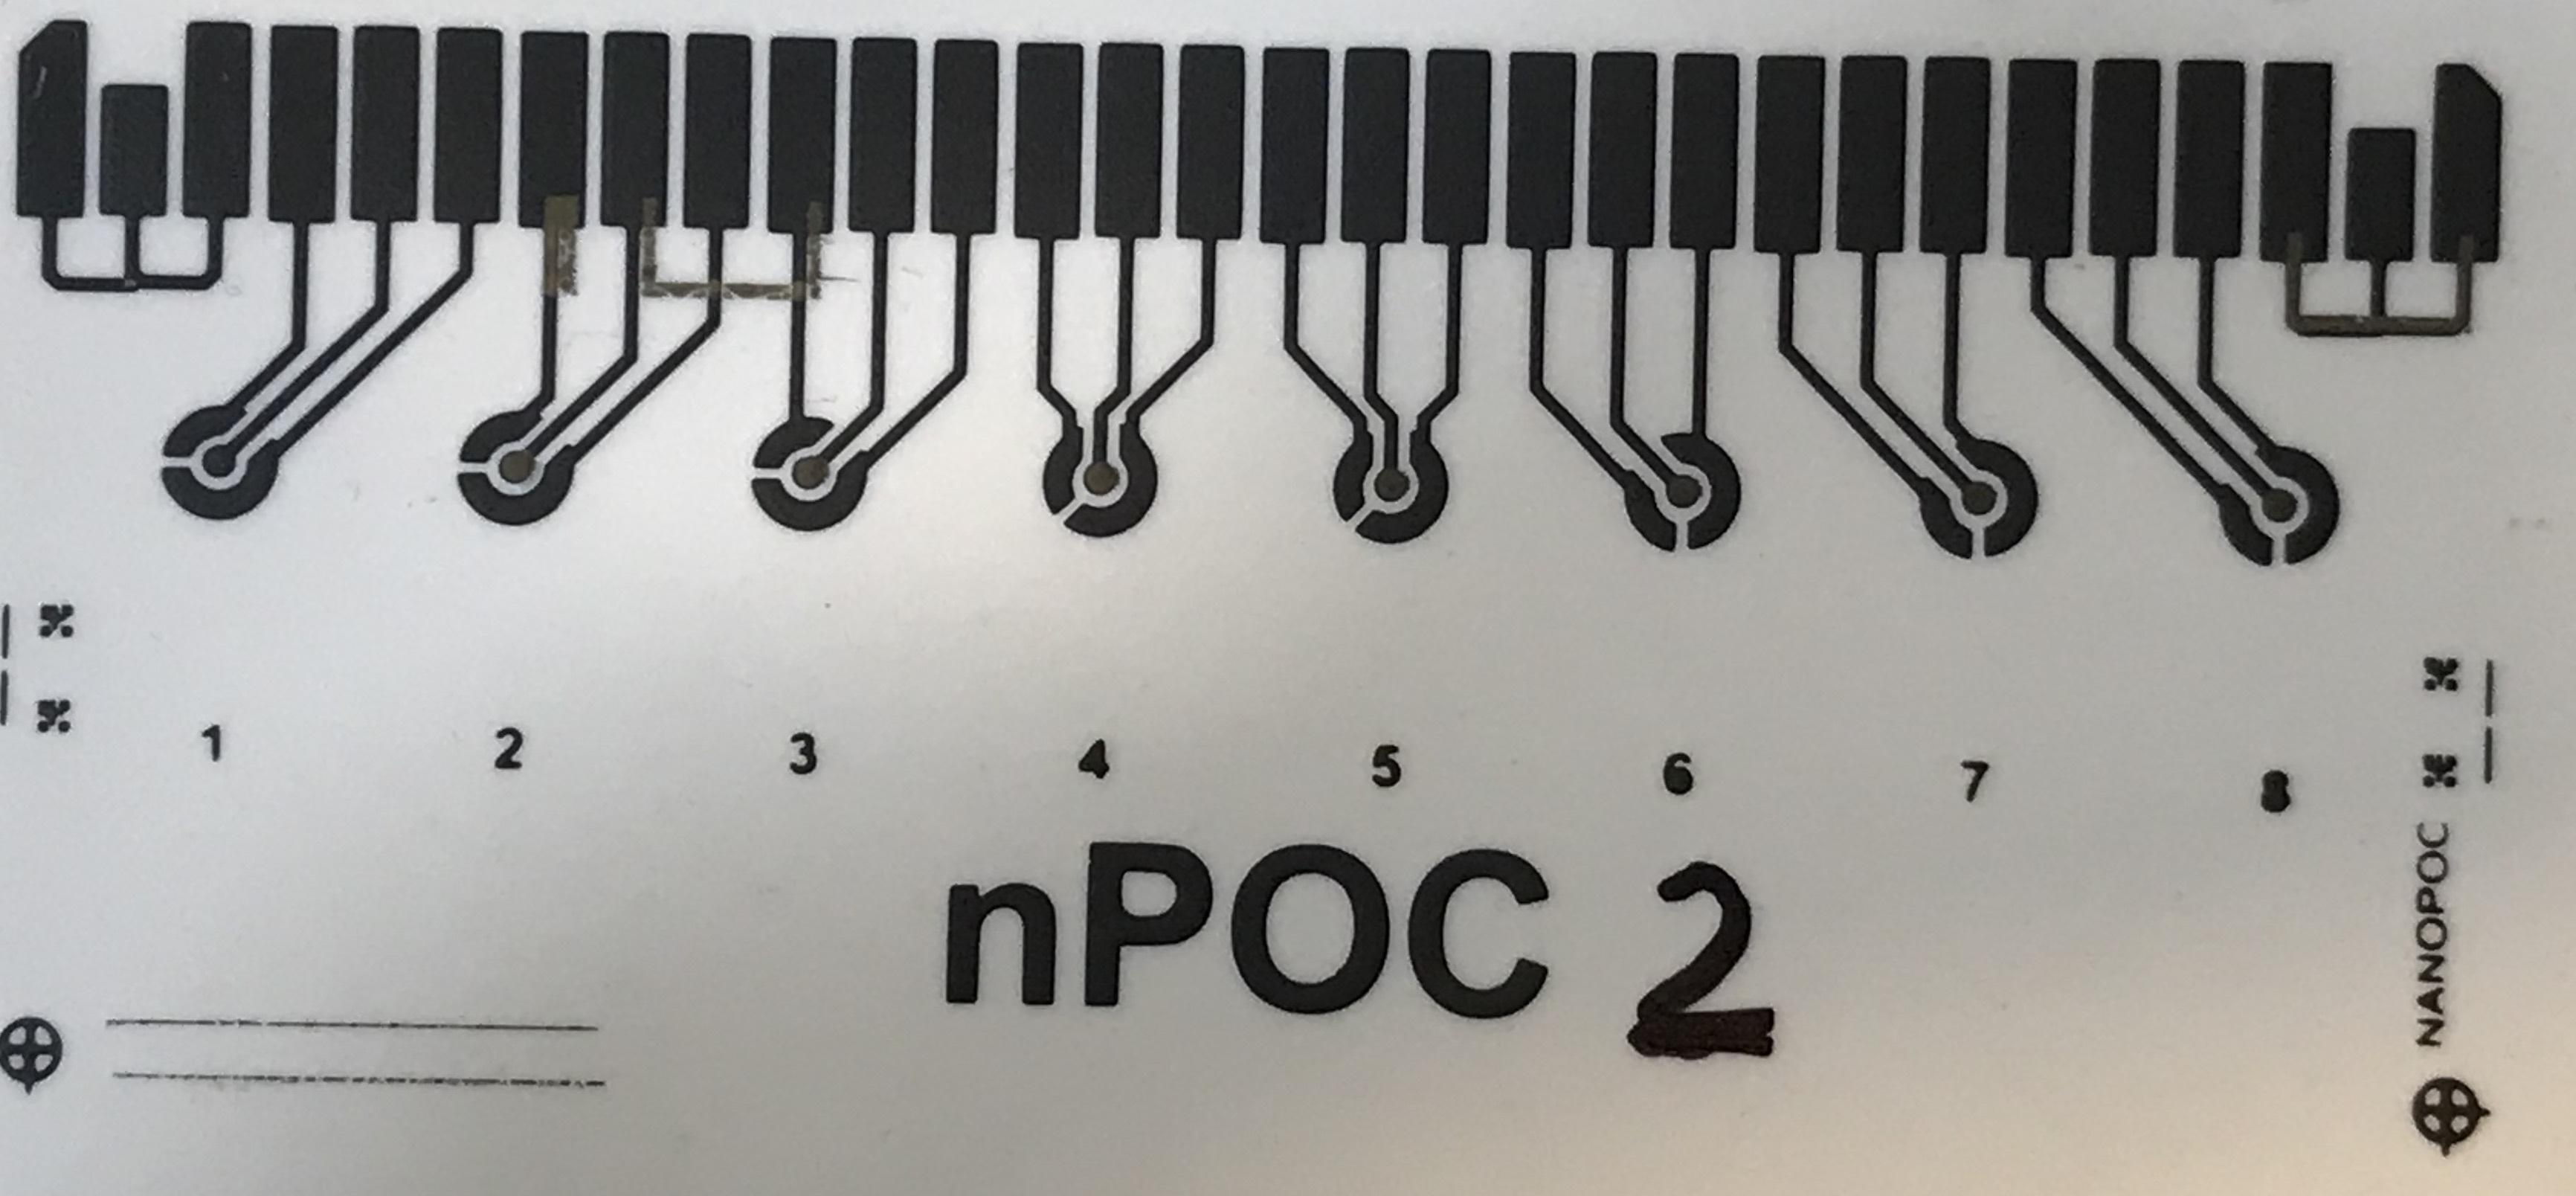
\includegraphics[width=0.5\textwidth]{Figuras/Figura_ejemplo_numeracion_nPoc}
  \caption{Ejemplo de numeración de sensor nPoc2}
  \label{fig:Figura_ejemplo_numeracion_nPoc}
\end{figure}

\subsection{Diseños de patrones de impresión}\label{subsec:diseno_impresion}
Una vez obtenidas las medidas necesarias de los sensores se procede a diseñar los patrones de impresión. Para esto se utilizó el editor profesional de vectores gráficos libre y de código abierto InkScape \cite{Inkscape} (Figura ~\ref{fig:Figura_Inkscape}).

\begin{figure}[H]
  \centering
    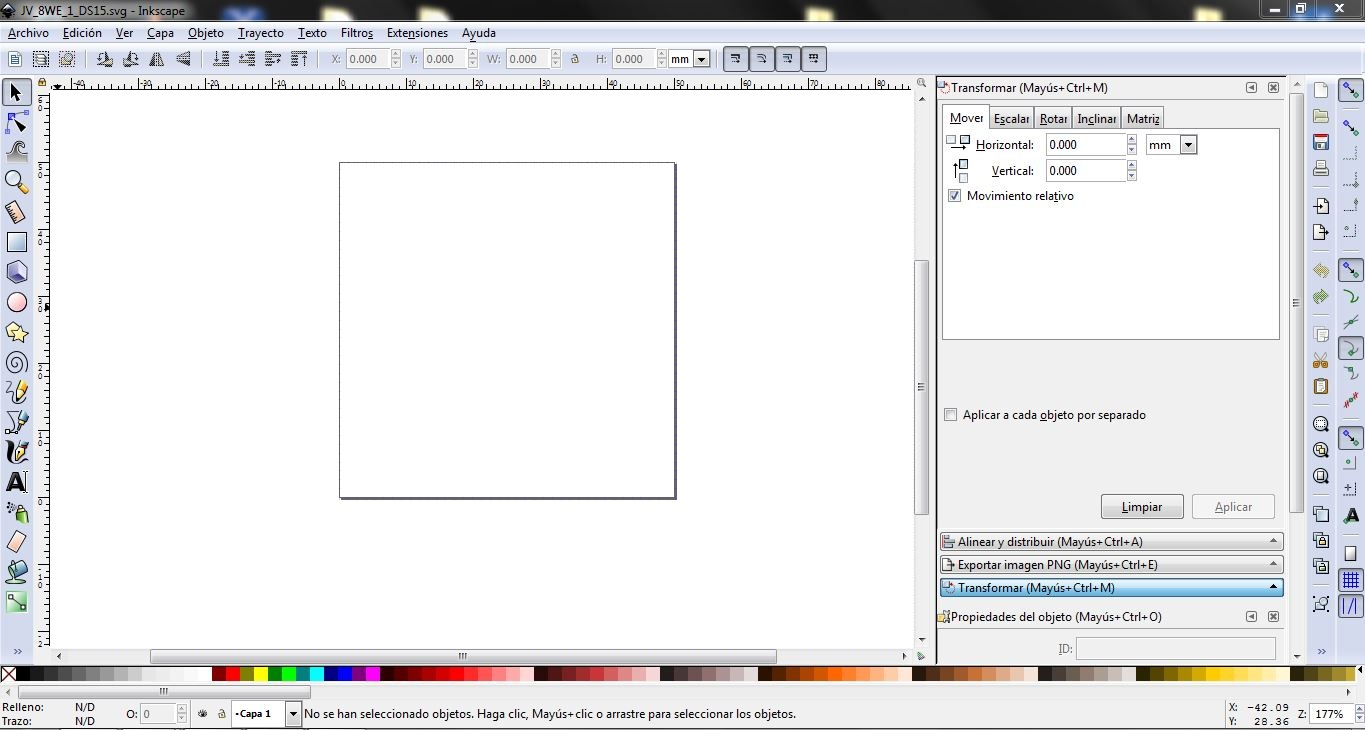
\includegraphics[width=0.65\textwidth]{Figuras/Figura_Inkscape}
  \caption{Editor profesional de vectores gráficos libre y de código abierto.}
  \label{fig:Figura_Inkscape}
\end{figure}

 Se realizaron cuatro dibujos con dos resoluciones posibles. Los primeros dibujos corresponden a un círculo de 1 mm y 1,1 mm de diámetro, el tamaño de un \emph{WE} y 100 $\mu$m más en el segundo. Con esto se pretende establecer si utilizando el mismo diámetro se logra una cobertura óptima con la tinta de nanopartículas de oro o se precisa agregar un \textit{offset}. Los otros dos dibujos constan de un arreglo de ocho círculos de 1 mm de diámetro, espaciados 9 mm entre sí y un arreglo de ocho círculos de 1,1 mm de diámetro, con el mismo espaciado (Figura ~\ref{fig:Figura_Diseno_Circulos}). Las resoluciones utilizadas fueron de 1693.33 y 1270 dpi, posteriormente se explicará la razón de dichas resoluciones.

\begin{figure}[H]
  \centering
    
\includegraphics[width=0.5\textwidth]{Figuras/Figura_Diseno_Circulos}
  \caption{Diseños de impresiones en 1 y 1,1 mm.}
  \label{fig:Figura_Diseno_Circulos}
\end{figure}

Dado que el software de la impresora (\textit{Dimatix Drop Manager}) no detecta imágenes a color o a escala de grises, se deben convertir las imágenes en archivos de 1 bit monocromático. De esta forma lo único presente en la imagen son pixeles blancos o negros, correspondiendo a donde debe eyectarse o no una gota de tinta. El formato que puede guardar imágenes de 1 bit es el Windows bitmap (ó BMP por sus siglas en inglés), y por esto es el único formato externo soportado por el \textit{Dimatix Drop Manager}. La conversión a formato BMP se realiza mediante el Software \textit{Microsoft Paint}. Realizando un zoom sobre la misma imagen en formato PNG y BMP, se pueden apreciar las diferencias a simple vista (Figura ~\ref{fig:Figura_comparacion_png_bmp}).

\begin{figure}[H]
  \centering
    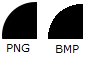
\includegraphics[width=0.5\textwidth]{Figuras/Figura_comparacion_png_bmp}
  \caption{Comparación archivos PNG y BMP.}
  \label{fig:Figura_comparacion_png_bmp}
\end{figure}

Una vez obtenidos los archivos en el formato correcto se puede proceder a la preparación y puesta a punto de los parámetros de la impresora.


\section{Puesta a punto y calibraci\'on de impresora}\label{sec:calib_impresora}
Luego de preparar, colocar y configurar el cartucho de tinta y el sustrato (ver \hyperref[chap:apendiceA]{Anexo A}) se debe agregar el diseño o patrón que se quiere imprimir.

Para esto el software DMP ofrece dos opciones. La primera permite realizar el dibujo con el mismo programa agregando posiciones (coordenadas X e Y) y los espesores deseados; la segunda permite importar imágenes con formato BMP monocromático. La creación de diseños mediante el software de DMP solo permite formas básicas y sobre todo confomadas por líneas rectas. Para dibujos más complejos se recomienda el procedimiento de diseño externo explicado en el apartado de diseño de patrones de impresión (Capítulo 3, \hyperref[subsec:diseno_impresion]{apartado 3.1.2}).

Para cualquiera de las dos opciones se les puede agregar coordenadas de referencia, utilizadas para ubicar la impresión en el sustrato y un $``$\textit{Leader Bar}$"$ con la posibilidad de configurar su ancho y su distancia ($``$\textit{Gap}$"$) con el diseño a imprimir. Esta última función es un procedimiento comúnmente utilizado para mantener los inyectores activos y su velocidad de caída uniforme al momento de la impresión, mejorando la calidad del patrón. Se debe tener en consideración que los $``$\textit{Leader Bars}$"$ deben ubicarse dentro del sustrato, de lo contrario se estará eyectando tinta sobre la platina de la impresora (Figura ~\ref{fig:Figura_Leader_Bar}).

\begin{figure}[H]
  \centering
    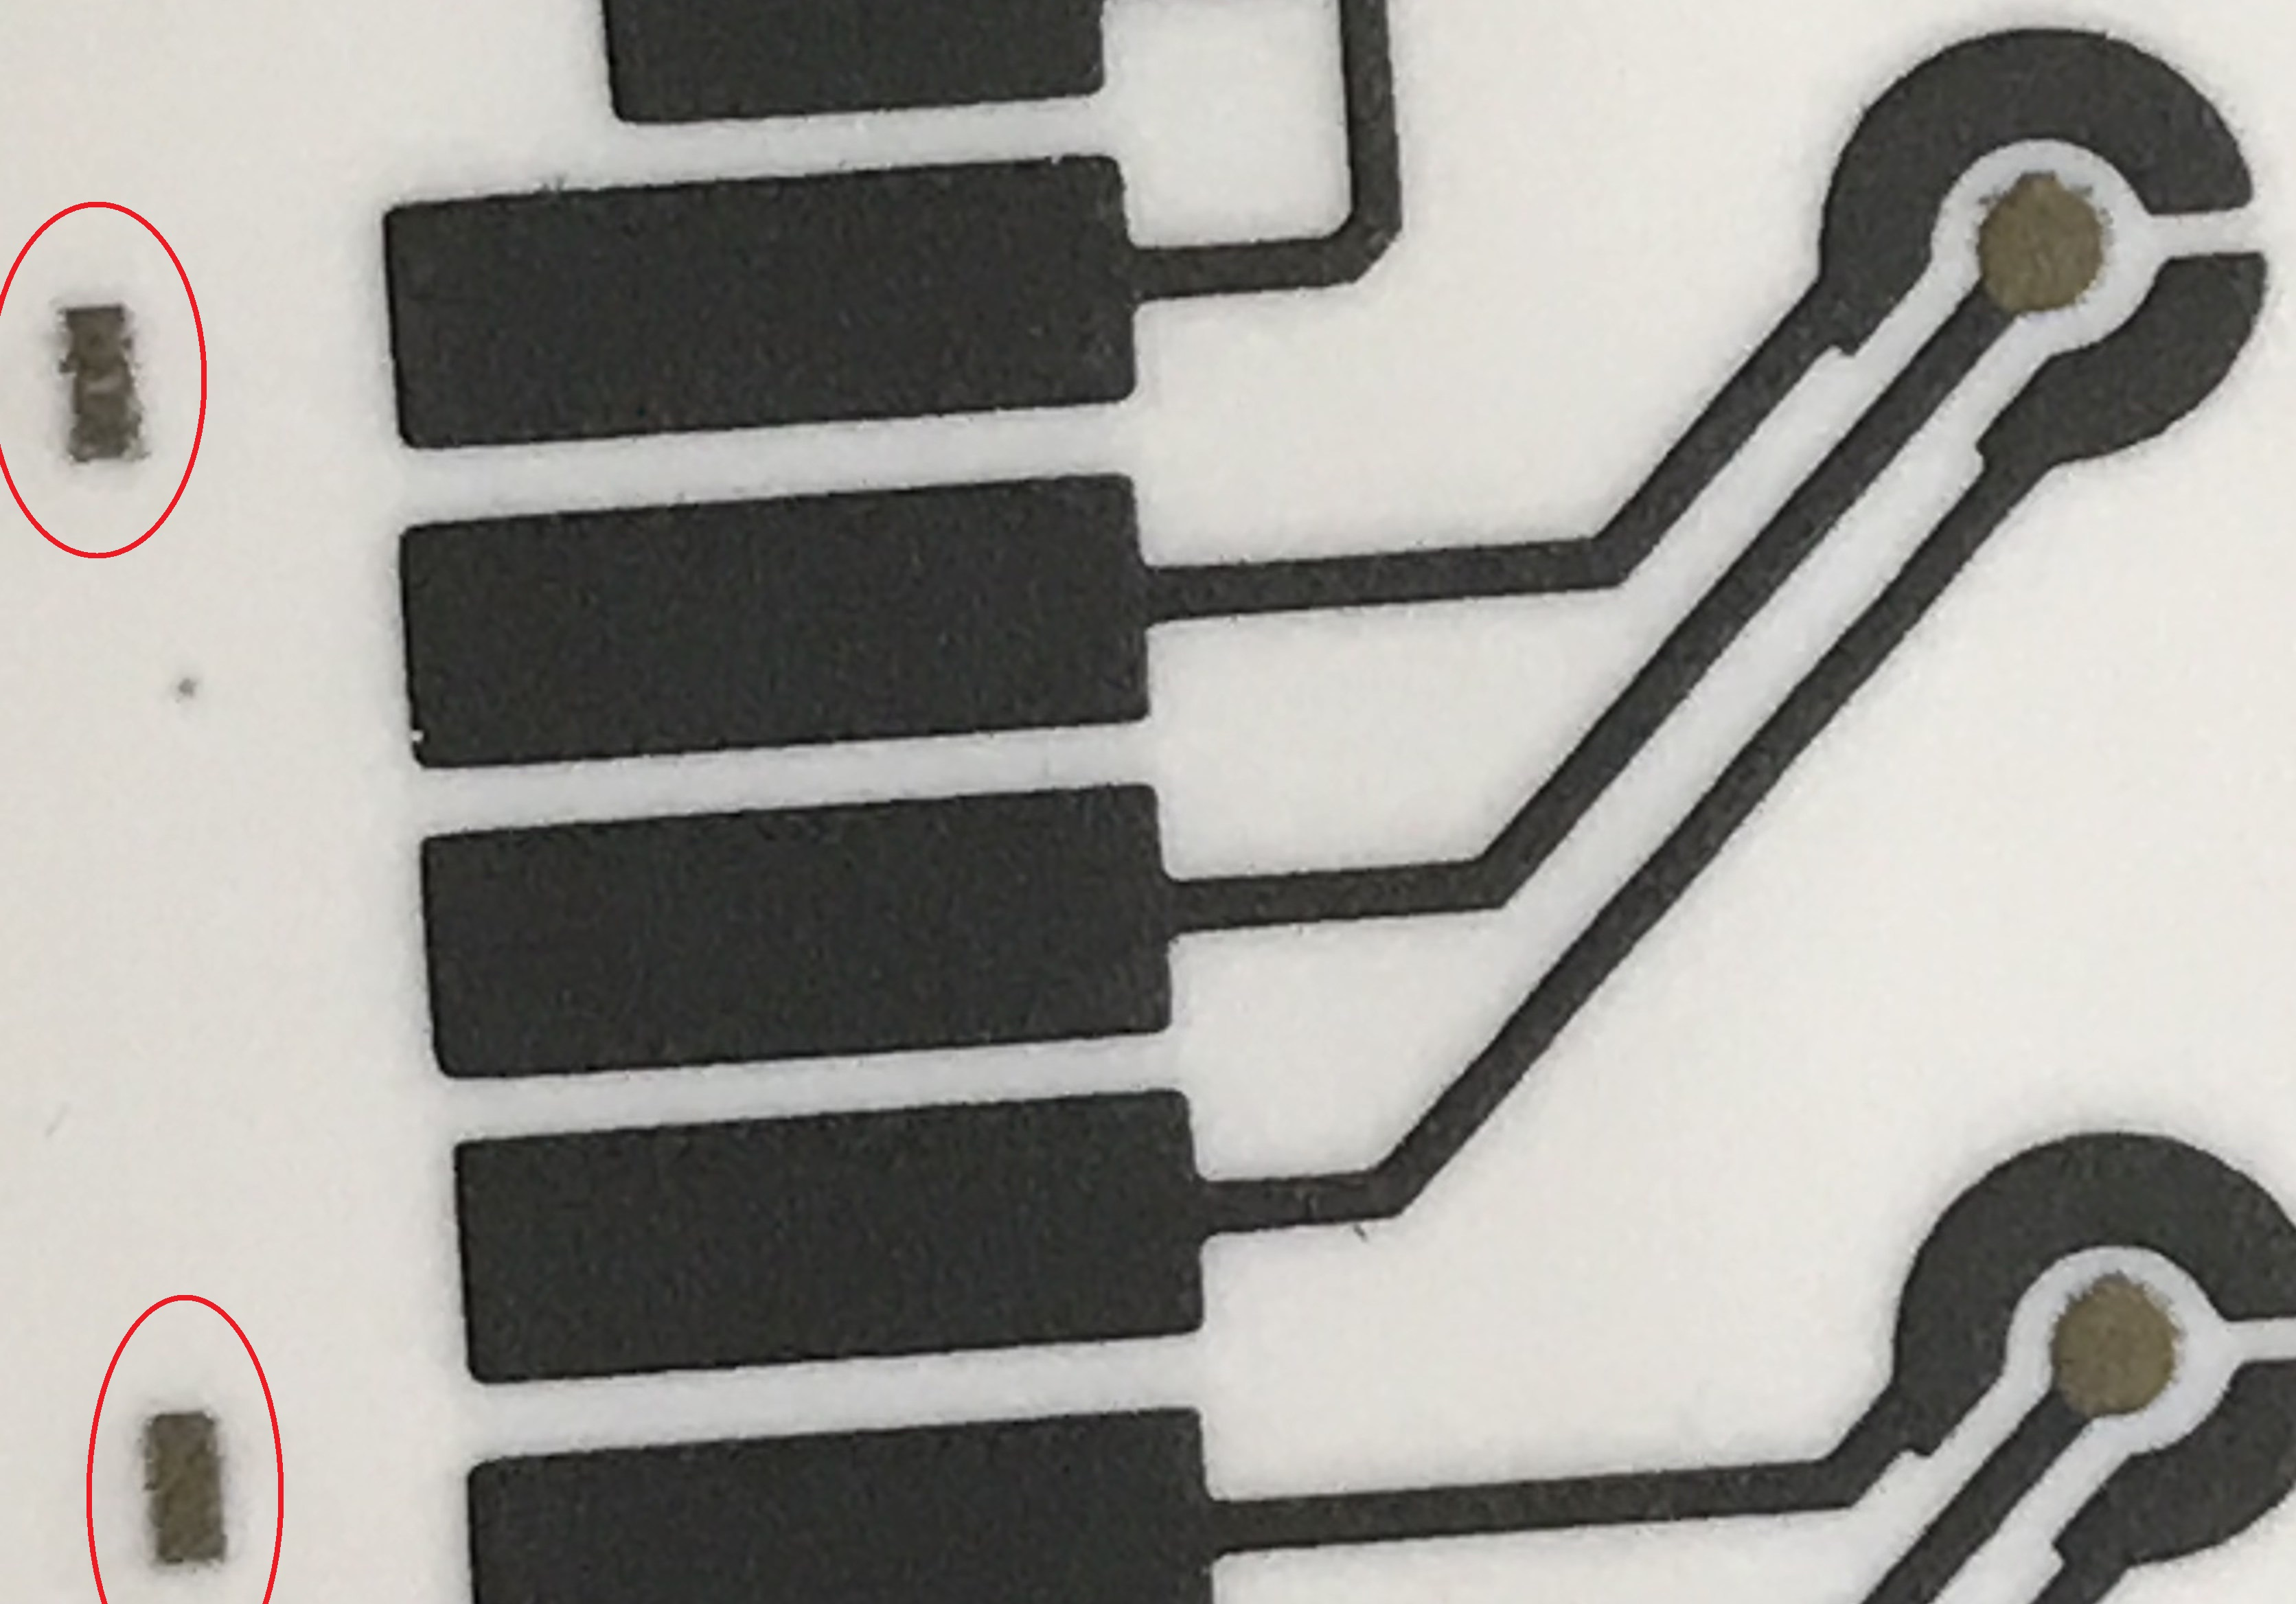
\includegraphics[width=0.5\textwidth]{Figuras/Figura_Leader_Bar}
  \caption{$``$\textit{Leader Bars}$"$ impresos sobre sustrato.}
  \label{fig:Figura_Leader_Bar}
\end{figure}

Llegado este momento, si no se realizó anteriormente, es aconsejable calibrar las tensiones de eyección de los inyectores (del inglés $``$\textit{Nozzles}$"$) que serán utilizados mediante el $``$\textit{Drop Watcher}$"$ (Figura ~\ref{fig:Figura_nozzles}). Este sistema consta de una cámara orientada a 45º del plano horizontal con foco en los eyectores del cabezal que ,mediante una luz estroboscópica, permite realizar fotografías o filmaciones sobre el funcionamiento de los orificios del cabezal (Eyección de gotas).

\begin{figure}[H]
  \centering
    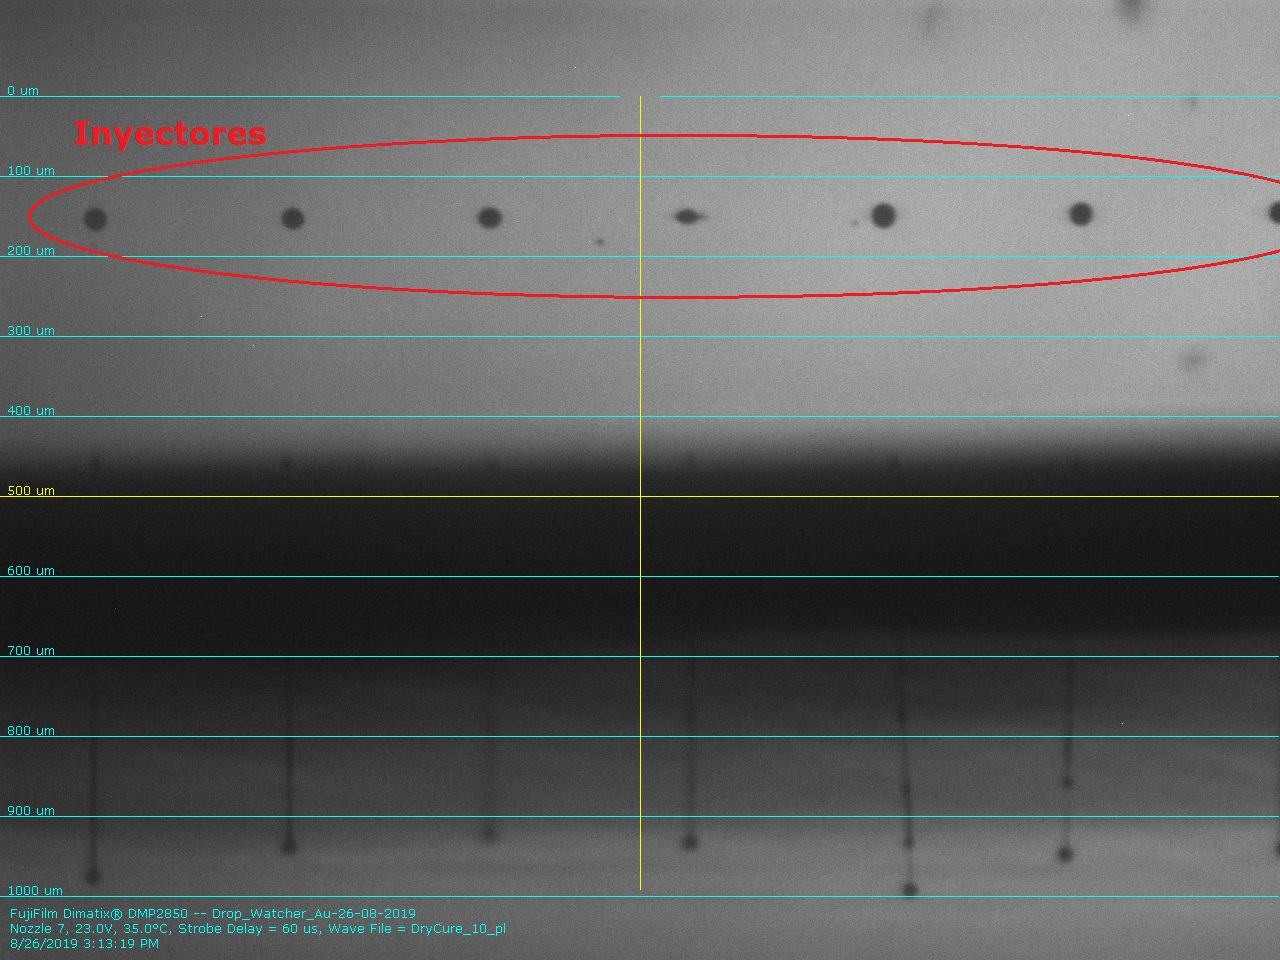
\includegraphics[width=0.5\textwidth]{Figuras/Figura_nozzles}
  \caption{Inyectores vistos desde cámara $``$\textit{Drop Watcher}$"$.}
  \label{fig:Figura_nozzles}
\end{figure}

Luego, utilizando la cámara fiducial, se realizan los procesos de alineación de gotas, sustrato y se fijan las coordenadas donde comienza la impresión.

La alineación del sustrato se logra mediante la calibración de \textit{Theta}. Para este procedimiento se deben seleccionar dos puntos que se encuentren alineados sobre el sustrato. En este caso, la impresión de carbono incluye distintos puntos de alineación, utilizando los más pequeños para obtener una mayor precisión, minimizando el error por el ancho mínimo de impresión de la fabricación serigráfica (Figura ~\ref{fig:Figura_alineacion_theta}).

\begin{figure}[H]
  \centering
    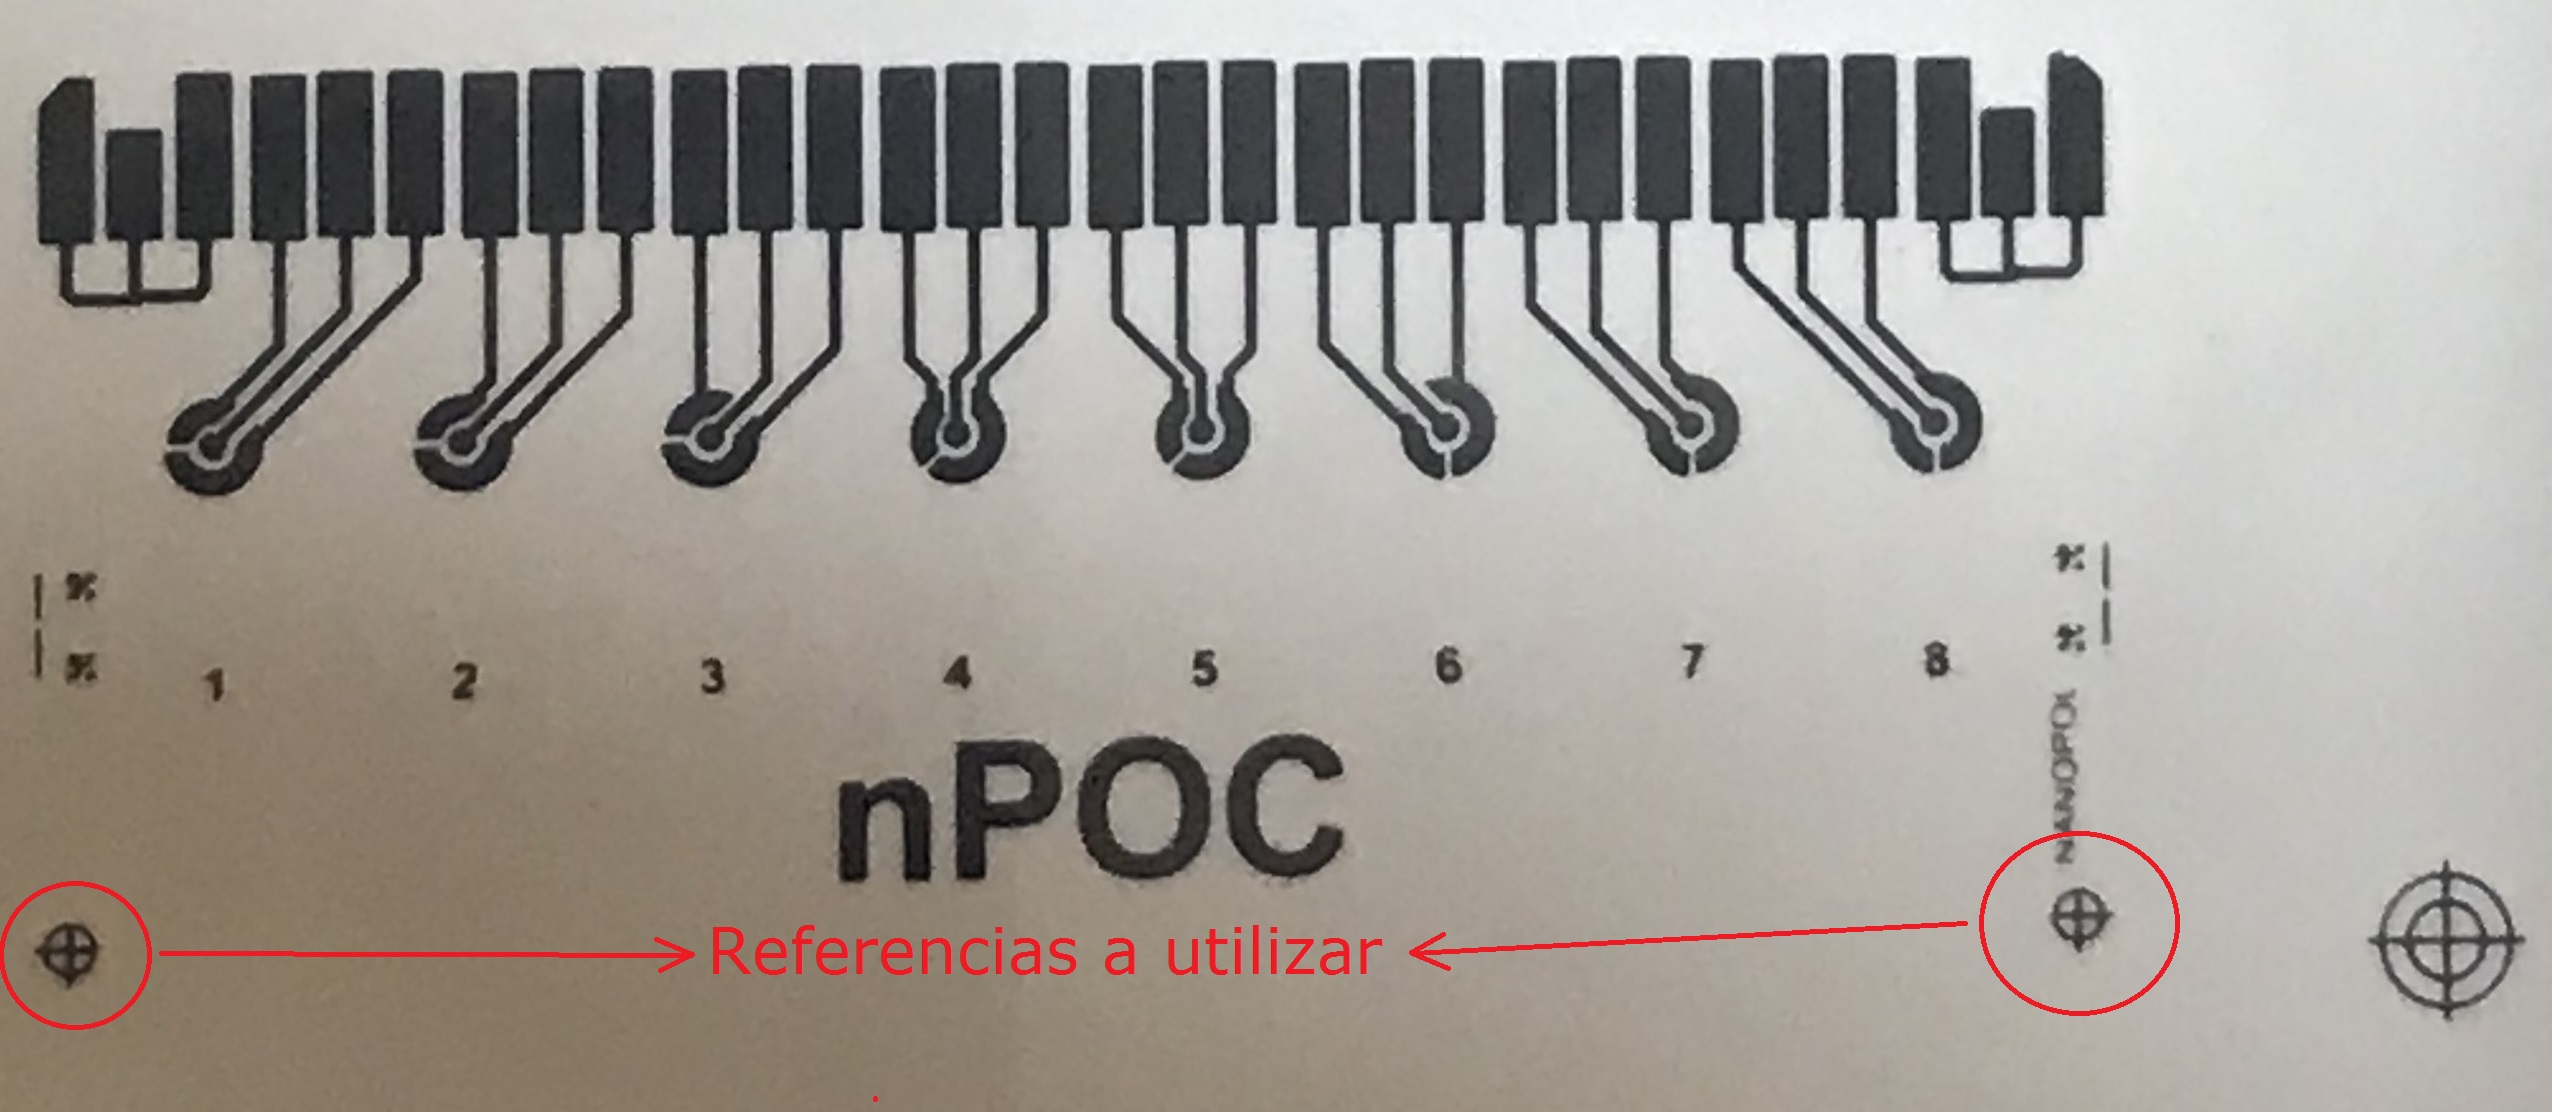
\includegraphics[width=0.5\textwidth]{Figuras/Figura_alineacion_theta}
  \caption{Referencias a utilizar para la calibración de \textit{Theta}.}
  \label{fig:Figura_alineacion_theta}
\end{figure}

Si bien, a simple vista, los objetos de alineación parecen de trazos finos y regulares, al utilizar la cámara fiducial se ve que no es sencillo determinar el punto medio (Figura ~\ref{fig:Figura_alineacion_theta2}).

\begin{figure}[H]
  \centering
    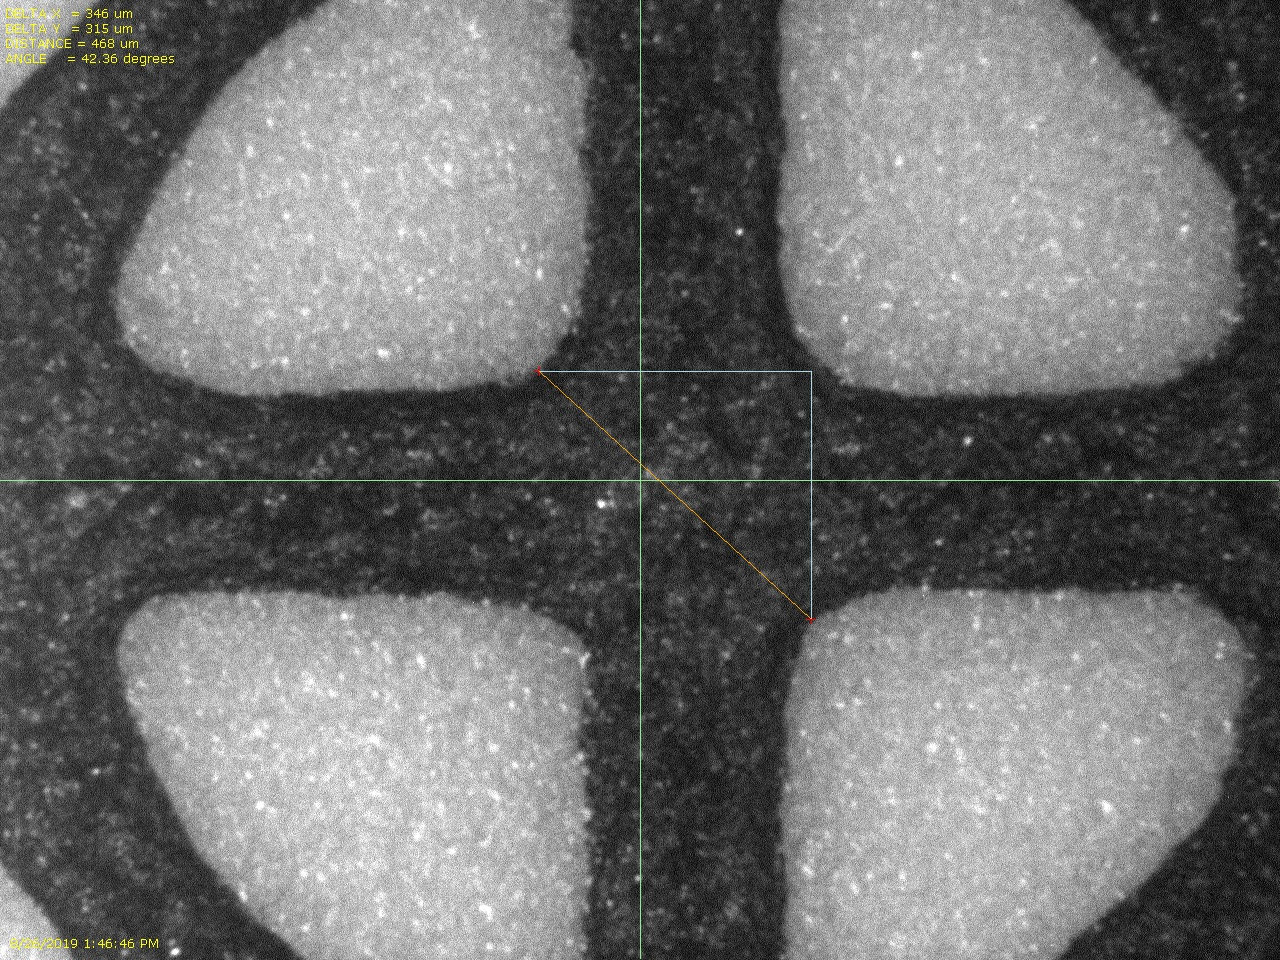
\includegraphics[width=0.4\textwidth]{Figuras/Figura_alineacion_theta2}
  \caption{Objeto de alineación visto con cámara fiducial.}
  \label{fig:Figura_alineacion_theta2}
\end{figure}

Seguido a alinear el sustrato, se debe definir el espaciado entre gotas que se utilizará al imprimir. Este parámetro es identificado como $``$\textit{Drop Spacing}$"$ (Desde ahora \emph{DS}) y, para determinarlo, se utilizó un patrón de gotas con los diferentes espaciados permitidos por la impresora, llamado $``$\textit{Line Pattern}$"$(Figura ~\ref{fig:Figura_Line_Pattern_Micro50X}). Luego de imprimir, se decide que $``$\textit{Drop Spacing}$"$ genera la línea mejor definida, tanto en continuidad como en homogeneidad de ancho de línea y espesor, sobre el sustrato a utilizar. Para la tinta de oro sobre \textit{Valox} se decidió utilizar un espaciado de 15 $\mu$m entre gotas, dado que este muestra una línea continua sin generar $``$\textit{Clusters}$"$ de tinta.

\begin{figure}[H]
  \centering
    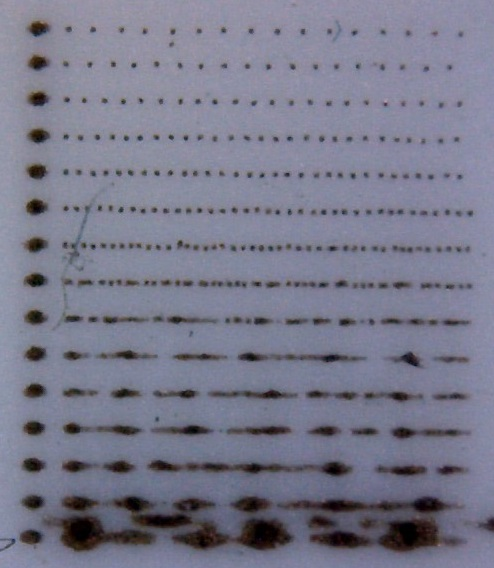
\includegraphics[width=0.35\textwidth]{Figuras/Figura_Line_Pattern_Micro50X}
  \caption{$``$\textit{Line Pattern}$"$, vista con microscopio de 50X.}
  \label{fig:Figura_Line_Pattern_Micro50X}
\end{figure}

Una vez definido el \emph{DS}, se ajusta la resolución del diseño que se desea imprimir. En el caso del $``$\textit{Drop Spacing}$"$ de 15 $\mu$m entre gotas, se utiliza una resolución de 1693.33 puntos por pulgada ($``$\textit{dpi}$"$). El manual de instrucciones de la impresora \cite{DimatixUM} brinda una tabla con la resolución que debe tener el diseño y el ángulo al que debe configurarse el cartucho para cada \emph{DS} (Figura ~\ref{fig:Figura_Tabla_angulos}).

\begin{figure}[H]
  \centering
    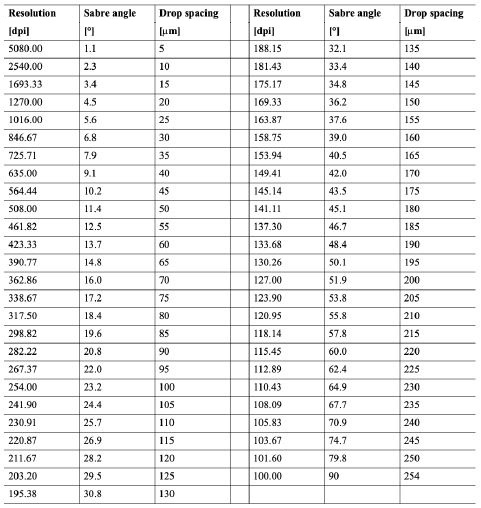
\includegraphics[width=0.5\textwidth]{Figuras/Figura_Tabla_angulos}
  \caption{Tabla de resoluciones y ángulos para cada \emph{DS}.}
  \label{fig:Figura_Tabla_angulos}
\end{figure}

A continuación se debe realizar la calibración de $``$\textit{Drop Offset}$"$. Este procedimiento compensa el error entre el punto en que la cámara fiducial está captando y la posición en la que el cartucho está imprimiendo. Es decir, compensa el vuelo de las gotas de tinta entre su eyección del cabezal hasta su impacto con el sustrato. Para esto, la impresora realiza una línea continua de 10 mm en el eje X seguido de un punto a 1 mm de la línea. La calibración se realiza una vez que se ubica este punto en la cámara fiducial y se hace $``$\textit{click}$"$ sobre él, lo más centrado posible (Figura ~\ref{fig:Figura_prueba_Drop_Spacing}).

\begin{figure}[H]
  \centering
    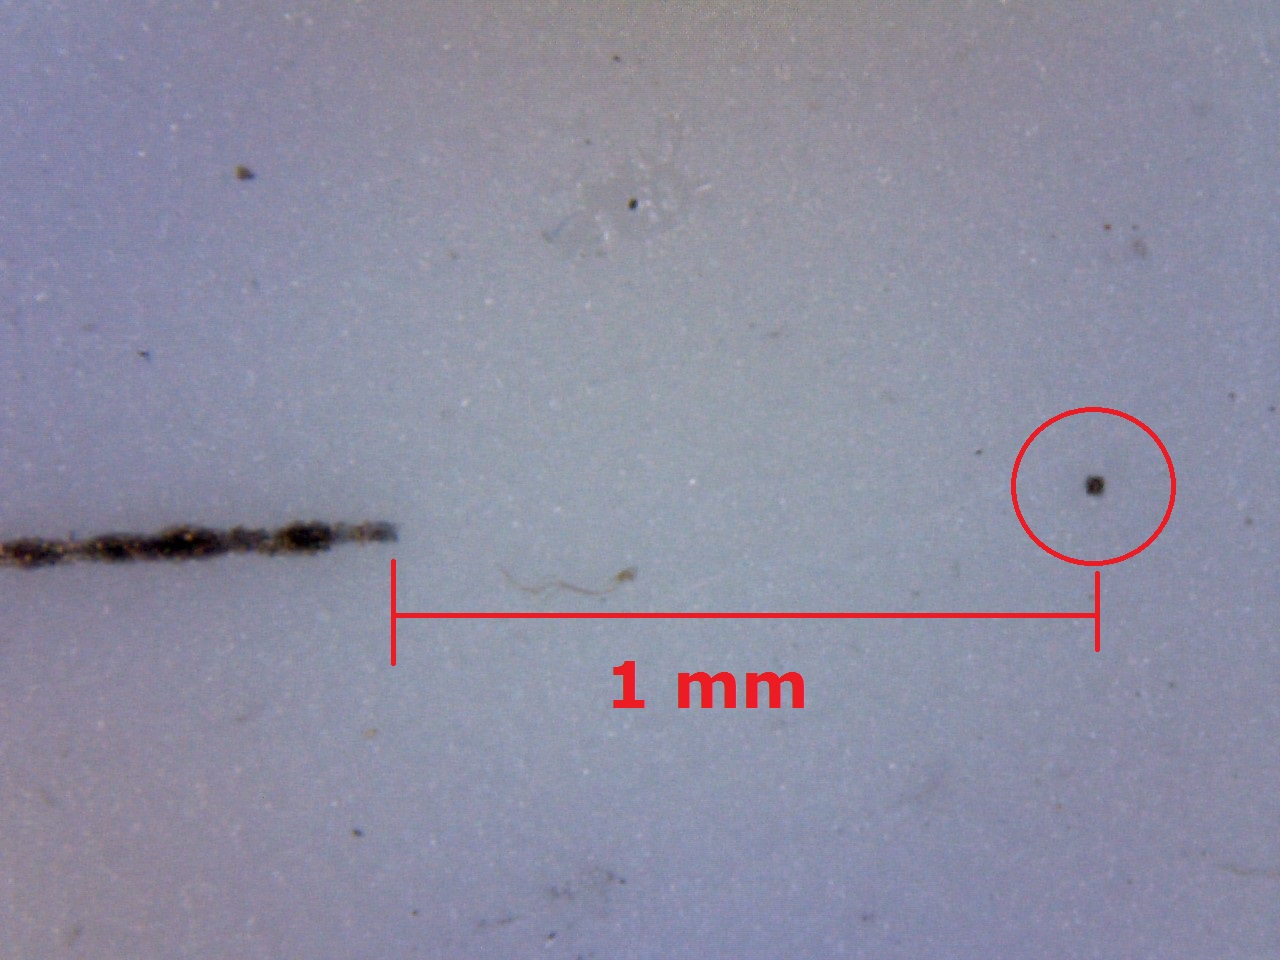
\includegraphics[width=0.5\textwidth]{Figuras/Figura_prueba_Drop_Spacing}
  \caption{Fin de línea y punto de procedimiento $``$\textit{Drop Offset}$"$, vista con microscopio de 1000X.}
  \label{fig:Figura_prueba_Drop_Spacing}
\end{figure}

La cámara fiducial es un elemento que forma parte del carrete donde se coloca el cartucho (Figura ~\ref{fig:Figura_Camara_Fiducial}). Esta es utilizada para los procedimientos de alineación del sustrato,  la calibración del tiempo de vuelo de las gotas eyectadas, el chequeo del sustrato y las impresiones sobre el mismo o mediciones sobre la superficie colocada sobre la platina. Tiene un campo de visión de 1,62 mm de ancho y 1,22 mm de alto, con una resolución de 2,54 $\mu$m por pixel.

\begin{figure}[H]
  \centering
    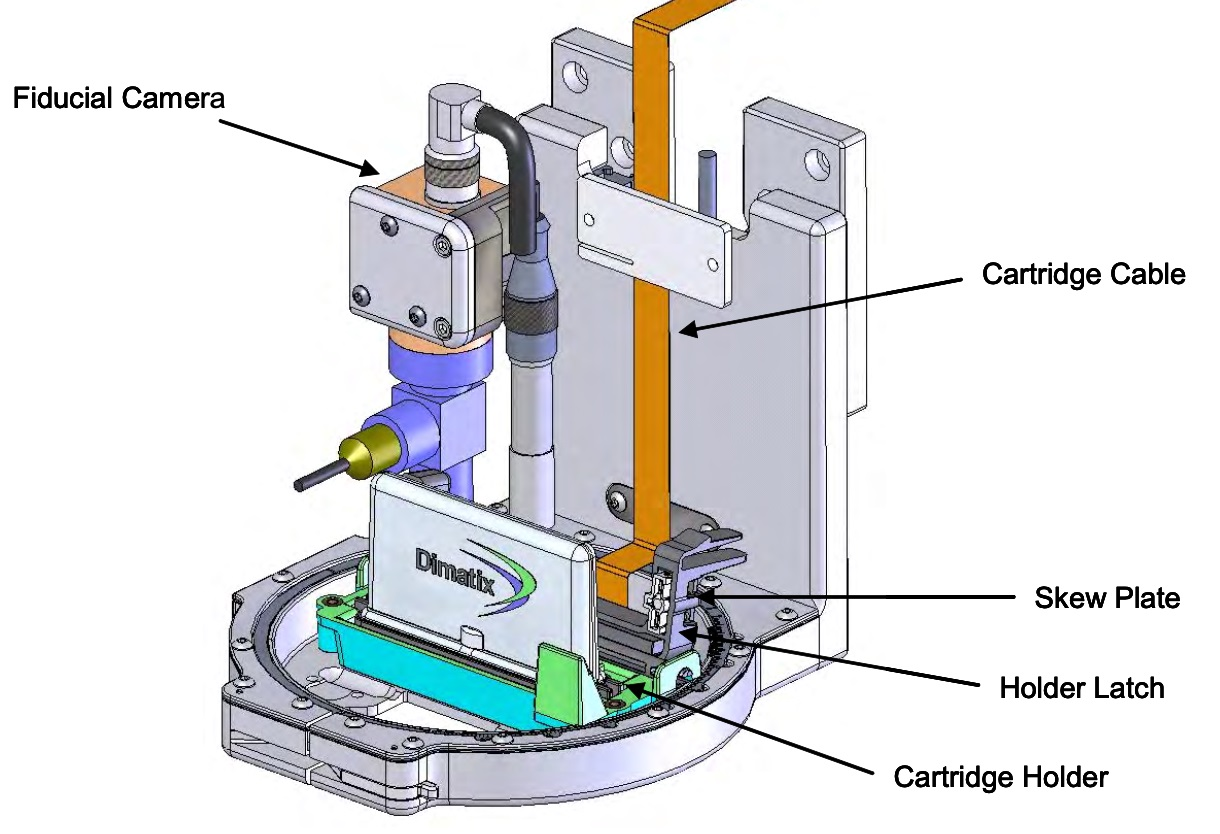
\includegraphics[width=0.5\textwidth]{Figuras/Figura_Camara_Fiducial}
  \caption{Ilustración de los distintos componentes del carrete de la impresora.}
  \label{fig:Figura_Camara_Fiducial}
\end{figure}

Como última configuración antes de comenzar la impresión, se deben definir las coordenadas del sustrato donde se comenzará a imprimir ($``$\textit{Print Origin}$"$) o de referencia, que concordarán con las definidas en el diseño ($``$\textit{Reference Point}$"$).

Si se decide utilizar el punto donde se comenzará a imprimir, se debe elegir la función \textit{Set Print Origin} de la cámara fiducial. En cambio, si se desea referenciar un punto del diseño con el sustrato, debe configurarse la función \textit{Set Reference Point} (Figura ~\ref{fig:Figura_Ventana_Camara_Fiducial}). Al utilizar la última función debe tenerse en cuenta que el punto de referencia debe estar definido en el diseño antes de cargarlo en la solapa de imagen a imprimir del software \textit{DMP}.

\begin{figure}[H]
  \centering
    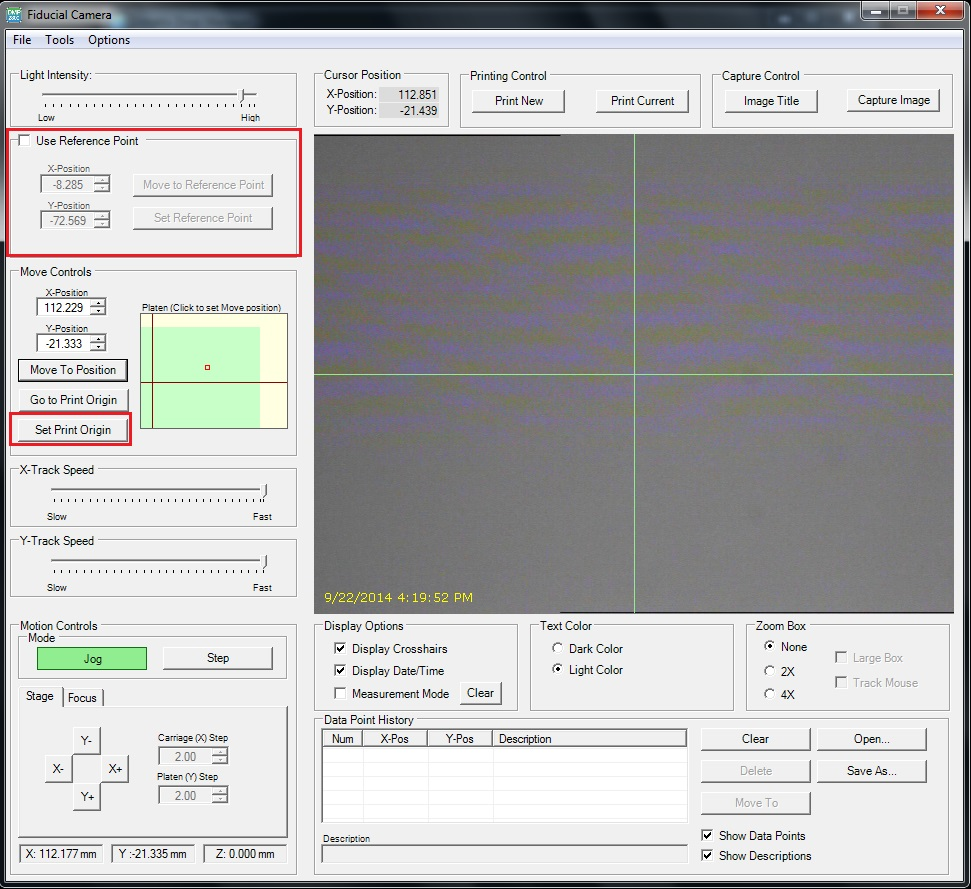
\includegraphics[width=0.5\textwidth]{Figuras/Figura_Ventana_Camara_Fiducial}
  \caption{Ventana de cámara fiducial con opciones para \textit{Print Origin} y \textit{Reference Point}.}
  \label{fig:Figura_Ventana_Camara_Fiducial}
\end{figure}

Para este trabajo se decidió utilizar como punto de referencia el centro del primer círculo, alineándolo con el electrodo de trabajo 1 del sensor. De esta manera, los otros 7 círculos quedaron alineados con su respectivo electrodo.

\section{Impresiones}
Como primera prueba, se realizó la impresión de un círculo de 1 mm de diámetro sobre la tinta de carbono y sobre el sustrato \textit{Valox}, para verificar el comportamiento de la tinta de oro sobre ambas superficies (Figura ~\ref{fig:Figura_Prueba_Sobre_Sustratos}).

\begin{figure}[H]
  \centering
    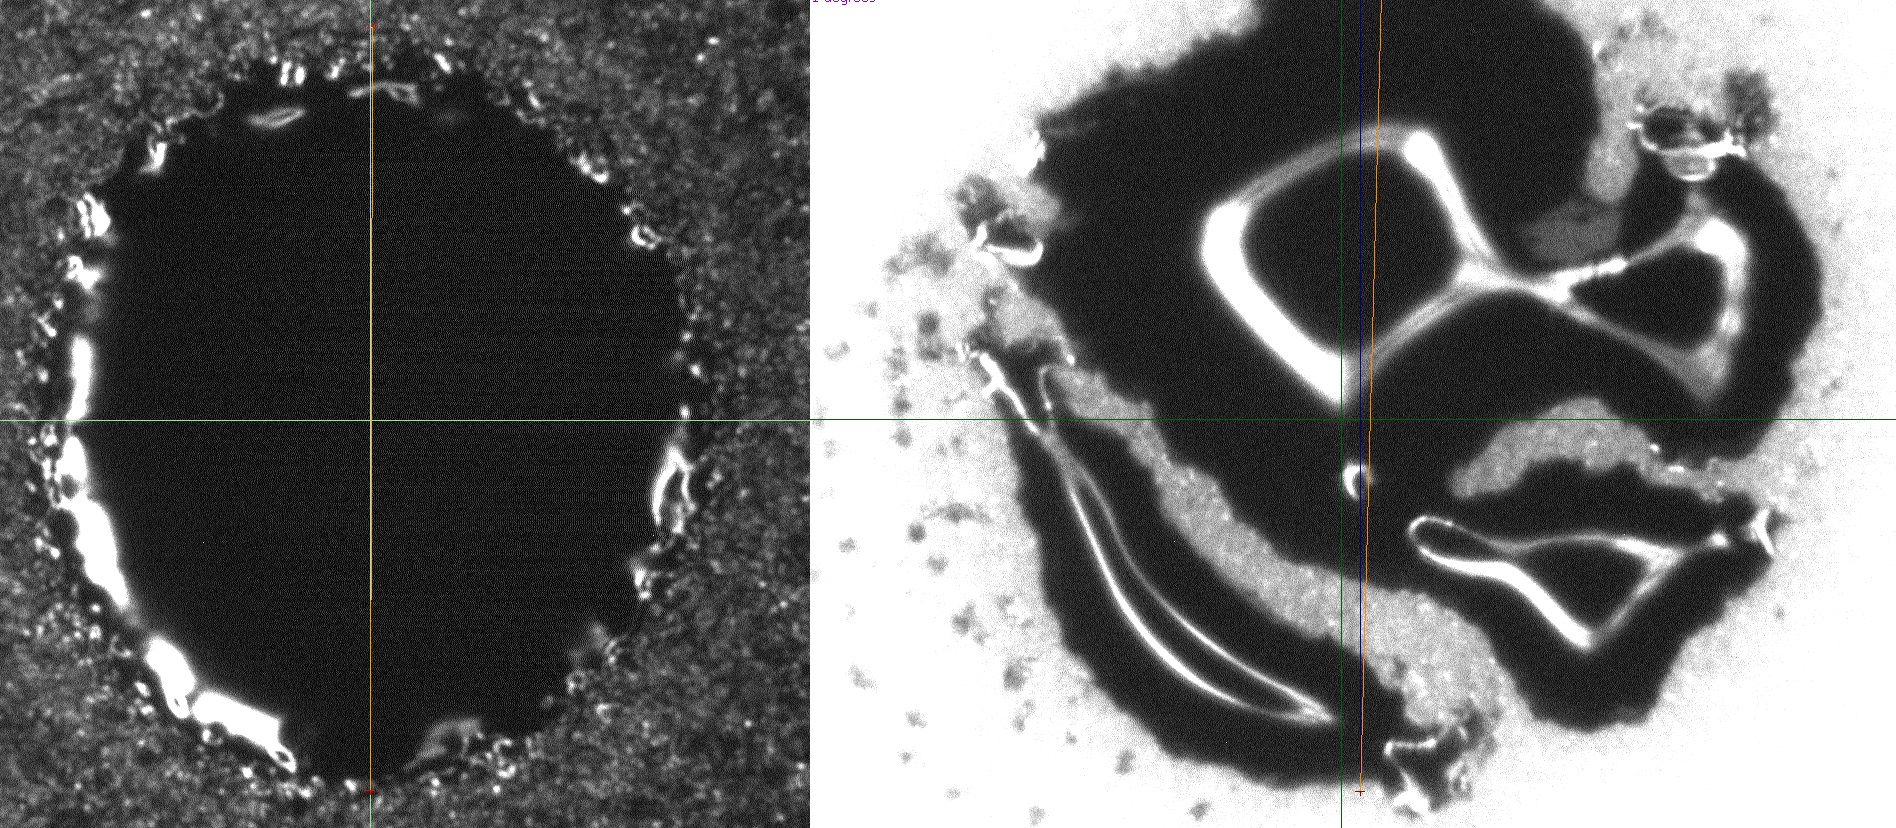
\includegraphics[width=0.5\textwidth]{Figuras/Figura_Prueba_Sobre_Sustratos}
  \caption{Prueba tinta de oro sobre tinta de carbono y sustrato \textit{Valox}.}
  \label{fig:Figura_Prueba_Sobre_Sustratos}
\end{figure}
Como se esperaba, la tinta de oro muestra un mejor anclaje sobre el carbono que sobre el sustrato.

La siguiente prueba fue alinear el punto de referencia con el dibujo a imprimir en el centro del primer electrodo de trabajo (WE1) del biosensor llamado \textit{nPoc1}, realizar la impresión de una capa de tinta y tomar el tiempo que tarde en absorberse la tinta (Figura ~\ref{fig:Figura_Primera_impresion_circulo}). Para obtener un promedio del tiempo necesario, se repite el mismo procedimiento de impresión en los ocho electrodos del \textit{nPoc1}.

\begin{figure}[H]
  \centering
    \includegraphics[width=0.5\textwidth]{Figuras/Figura_Primera_impresion_circulo}
  \caption{Primera impresión sobre electrodo de trabajo (WE1).}
  \label{fig:Figura_Primera_impresion_circulo}
\end{figure}

Se concluye que el tiempo promedio necesario para el secado de la tinta es de 10 minutos. La tinta no estará completamente seca y anclada hasta se realice el curado de la misma. Para el procedimiento de curado de la tinta de oro sobre sustrato \textit{Valox} se utiliza un \textit{Hot Plate} a 80ºC por 80 minutos (Figura ~\ref{fig:Figura_Hot_Plate}). 

\begin{figure}[H]
  \centering
    \includegraphics[width=0.4\textwidth]{Figuras/Figura_Hot_Plate}
  \caption{Curado de electrodos en \textit{Hot Plate}.}
  \label{fig:Figura_Hot_Plate}
\end{figure}

La segunda impresión se realiza con círculos de 1,1 mm de diámetro, para comparar los resultados con la impresión anterior. Se imprimen los 8 electrodos de trabajo del \textit{nPoc5}, uno a la vez. Como se puede observar (Figura ~\ref{fig:Figura_Segunda_Impresion_circulo}), la tinta que cae sobre el sustrato no se ancla correctamente generando \textit{clusters} de la misma fuera del \emph{WE}.

\begin{figure}[H]
  \centering
    \includegraphics[width=0.45\textwidth]{Figuras/Figura_Segunda_Impresion_circulo}
  \caption{Impresión de círculo de 1,1 mm sobre \emph{WE}.}
  \label{fig:Figura_Segunda_Impresion_circulo}
\end{figure}

Para aumentar el nivel de reproducibilidad a mayor escala, se diseña un patrón de ocho círculos de 1 mm de diámetro cada uno. El punto de referencia se centra en el primer círculo y se alinea con el centro del primer \emph{WE} del sustrato \textit{nPoc3}.

Al revisar la impresión se notan pequeñas desviaciones en la deposición de la tinta de oro, esto puede deberse a las variaciones que se obtienen por la impresión serigráfica del patrón de tinta de carbono. Sin embargo, no se detectan derrames de tinta considerables sobre el sustrato \textit{Valox} (Figura ~\ref{fig:Figura_impresion_8juntos}).

\begin{figure}[H]
  \centering
    \includegraphics[width=0.6\textwidth]{Figuras/Figura_impresion_8juntos}
  \caption{Comparación de impresión entre \emph{WE} 3 y 5.}
  \label{fig:Figura_impresion_8juntos}
\end{figure}

A continuación, se cura el biosensor sobre un \textit{Hot Plate} a 80ºC por 80 minutos. Se observa que la tinta toma un color más claro, semejante al color del oro puro (Figura ~\ref{fig:Figura_impresion_curado}).

\begin{figure}[H]
  \centering
    \includegraphics[width=0.45\textwidth]{Figuras/Figura_impresion_curado}
  \caption{Imágen con microscopio USB 1000X de \emph{WE} curado en \textit{Hot Plate}.}
  \label{fig:Figura_impresion_curado}
\end{figure}

Para la caracterización eléctrica se diseñó un patrón con la forma de conexión entre dos contactos de prueba del biosensor (Figura ~\ref{fig:Figura_contactos_prueba}).

\begin{figure}[H]
  \centering
    \includegraphics[width=0.45\textwidth]{Figuras/Figura_contactos_prueba}
  \caption{Contactos de prueba en biosensor.}
  \label{fig:Figura_contactos_prueba}
\end{figure}

El diseño tiene 2,5 mm de alto y 5,5 mm de largo, el ancho de las vías es de 0,4 mm. Para esta impresión no se utilizó punto de referencia sino que se agregó el punto de origen de impresión alineado con el comienzo de las vías de carbono. Se añadió 1 mm sobre los contactos para tener una mejor relación carbono-nanopartículas de oro. Dado el buen anclaje de la tinta de nanopartículas de oro sobre el carbono se obtuvo correctamente el diseño buscado, casi sin derrames (Figura ~\ref{fig:Figura_contactos_prueba_con_Oro}). Se imprimieron dos capas del diseño, ambas curadas en \textit{Hot Plate} a 80ºC por 80 minutos.

\begin{figure}[H]
  \centering
    \includegraphics[width=0.45\textwidth]{Figuras/Figura_contactos_prueba_con_Oro}
  \caption{Contactos de prueba con impresión de tinta con nanopartículas de oro.}
  \label{fig:Figura_contactos_prueba_con_Oro}
\end{figure}

Para tener mayor cantidad de pruebas en la caracterización electroquímica se realizaron impresiones con tinta de nanopartículas de oro sobre el sustrato \textit{Valox}, sin tinta de carbono (Figura ~\ref{fig:Figura_impresion_sustrato_valox_tinta_Oro}), sobre un sustrato PET (Tereftalato de polietileno) y una hoja de pulpa de celulosa (hoja de cuaderno convencional).

\begin{figure}[H]
  \centering
    \includegraphics[width=0.5\textwidth]{Figuras/Figura_impresion_sustrato_valox_tinta_Oro}
  \caption{Impresión sobre sustrato Valox.}
  \label{fig:Figura_impresion_sustrato_valox_tinta_Oro}
\end{figure}

Sobre el sustrato \textit{Valox} y la hoja de pulpa de celulosa se imprimieron dos círculos de 1 mm de diámetro separados 16 mm que luego fueron unidos por una línea de 17 mm de largo y 0,4 mm de ancho, de esta forma la tinta se imprimió desde la mitad de un círculo hasta la mitad del otro, asegurando la continuidad del material. Se imprimieron dos capas idénticas, para el sustrato \textit{Valox} se realizó un curado entre cada impresión en \textit{Hot Plate} a 80ºC por 80 minutos.

Para el sustrato PET se realizó un diseño diferente (Figura ~\ref{fig:Figura_impresion_sobre_PET}) debido a que no se tenía referencia de cómo se anclaría la tinta sobre la base. Se realizó un arreglo de seis dibujos en dos columnas, compuestos por dos cuadrados de 1 mm de lado separados 16 mm y una barra de 17 mm de largo y 0,4 mm de ancho. La separación entre columnas es de 65 mm y 20 mm entre filas. La separación en columnas se debe a que la mitad del sustrato se limpió superficialmente con alcohol etílico, de esta forma, se buscó obervar las diferencias entre el sustrato tratado y sin tratar. Se imprimieron dos capas idénticas con sus respectivos curados en \textit{Hot Plate} a 80ºC por 80 minutos.

\begin{figure}[H]
  \centering
    \includegraphics[width=0.5\textwidth]{Figuras/Figura_impresion_sobre_PET}
  \caption{Diseño impreso sobre sustrato PET.}
  \label{fig:Figura_impresion_sobre_PET}
\end{figure}

\section{Caracterizaciones}
\subsection{Caracterización eléctrica}
La caracterización eléctrica consta de la medición de resistencia a 4 puntas, explicada anteriormente en el Capítulo 2, \hyperref[subsec:carac_elec]{apartado 2.3.1}. Las mediciones de resistencia se hicieron sobre tinta de carbono, tinta de carbono más una capa y más dos capas de tinta de nanopartículas de oro curado.

Se debe tener en cuenta que los resultados obtenidos de esta medición se compone de un paralelo eléctrico entre la resistencia de la tinta de carbono y la resistencia de la tinta de nanopartículas de oro. Se obtuvo un descenso considerable de la resistencia (en comparación de un paralelo de dos resistencias de carbono) en concordancia con la teoría propuesta, dado que la resistividad del oro (2.44·10\textsuperscript{-8} Ohm·m) es mucho menor a la del carbono (3.5·10\textsuperscript{-5} Ohm·m) \cite{Resistividad}.

\subsection{Caracterización dimensional}
Para la caracterización dimensional se utilizó la cámara fiducial de la impresora \textit{Dimatix}, obteniendo las dimensiones de los \emph{WE} y las separaciones entre este, el \emph{CE} y el \emph{RE} (Figura ~\ref{fig:Figura_medicion_WE}).

\begin{figure}[H]
  \centering
    \includegraphics[width=0.5\textwidth]{Figuras/Figura_medicion_WE}
  \caption{Medición del diámetro del \emph{WE}.}
  \label{fig:Figura_medicion_WE}
\end{figure}

La rugosidad y los espesores de la película de carbono y de la película obtenida con la tinta de nanopartículas de oro se obtuvieron mediante un perfilómetro de contacto marca \textit{Bruker} modelo \textit{Dektak XT} con una punta \textit{Stylus} de 12,5  $\mu$m (Figura ~\ref{fig:Figura_Perfilometro}). La fuerza aplicada por la punta fue en ambos casos de 3 mgf.

\begin{figure}[H]
  \centering
    \includegraphics[width=0.5\textwidth]{Figuras/Figura_Perfilometro}
  \caption{Perfilómetro Dektak XT Advanced.}
  \label{fig:Figura_Perfilometro}
\end{figure}

Para dicha caracterización se determinó un recorrido de 2000 $\mu$m sobre el electrodo de trabajo durante 15 segundos y luego se seleccionó el área de interés para medir la rugosidad. Se tomaron tres valores sobre toda la muestra:

$\bullet$ El valor promedio de rugosidad máxima (Rz)

$\bullet$ El pico de rugosidad más alto (Rt)

$\bullet$ El valor promedio de rugosidad (Ra).
\\

Para la caracterización del espesor del \emph{WE} se fijó un recorrido de 1000 $\mu$m durante 15 segundos. El largo del recorrido se determinó en ese valor para poder obtener los escalones de subida/bajada y con esto poder obtener una referencia (Figura ~\ref{fig:Figura_grafico_perfilometro}). Para determinar el espesor de la tinta de oro se midió el espesor de un pad de carbono y el de un \emph{WE} con tinta de nanopartículas de oro. Haciendo la diferencia entre ambos se obtuvo el espesor de dos capas de tinta de oro impresas por \textit{Inkjet}.

\begin{figure}[H]
  \centering
    \includegraphics[width=0.8\textwidth]{Figuras/Figura_grafico_perfilometro}
  \caption{Gráfico de caracterización del espesor.}
  \label{fig:Figura_grafico_perfilometro}
\end{figure}

Para los mencionados estudios se utilizaron dos muestras, identificadas como cartuchos nPoc3 y nPoc5, teniendo dos capas curadas de 1 mm y 1,1 mm de diámetro (Tinta de nanopartículas de oro) respectivamente. De cada uno de ellos se utilizaron los electrodos de trabajo identificados como 3 y 4 para obtener un muestreo variado. Se realizaron dos mediciones sobre cada uno y luego se promediaron.

\subsection{Caracterización electroquímica}
La caracterización electroquímica se realizó sobre diferentes configuraciones de sustratos y tintas para obtener múltiples comparaciones de interés para el proyecto. Se listan las muestras por orden de prueba (Figura ~\ref{fig:Figura_pruebas_muestras}):

$\bullet$ Electrodo de película delgada de oro depositado por \textit{sputtering} sobre silicio. (Figura ~\ref{fig:Figura_pruebas_muestras} (a))

$\bullet$ Electrodo de película impresa con carbono por serigrafía sobre sustrato \textit{Valox}. (Figura ~\ref{fig:Figura_pruebas_muestras} (b))

$\bullet$ Electrodo de película impresa con tinta de carbono por serigrafía y con impresión de tinta de nanopartículas de oro de 1 mm de diámetro sobre sustrato \textit{Valox}. (Figura ~\ref{fig:Figura_pruebas_muestras} (c))

$\bullet$ Electrodo de película impresa con tinta de carbono por serigrafía y con impresión de tinta de nanopartículas de oro de 1,1 mm de diámetro sobre sustrato \textit{Valox}.

$\bullet$ Impresión de tinta de nanopartículas de oro sobre sustrato \textit{Valox}.

$\bullet$ Impresión de tinta de nanopartículas de oro sobre sustrato PET. (Figura ~\ref{fig:Figura_pruebas_muestras} (d))

$\bullet$ Impresión de tinta de nanopartículas de oro sobre sustrato de pulpa de celulosa. (Figura ~\ref{fig:Figura_pruebas_muestras} (e))

\begin{figure}[H]
  \centering
    \includegraphics[width=1\textwidth]{Figuras/Figura_pruebas_muestras}
  \caption{Muestras donde se realizó la caracterización electroquímica.}
  \label{fig:Figura_pruebas_muestras}
\end{figure}

Para que las pruebas sean comparables entre sí, se utilizó un contraelectrodo de platino de 2 cm\textsuperscript{2} de área y un electrodo de referencia de cloruro de mercurio(I) o \textit{Calomel} saturado de la firma \textit{Cole-Parmer} (Hg\textsubscript{2}Cl\textsubscript{2}), ambos externos a las muestras. El reservorio de la celda electroquímica fue fabricada en acrílico con un volumen aproximado de 3 ml. Posee un orificio en la parte inferior donde pueden colocarse sellos de polipropileno. En los experimentos se utilizó un sello de 1 mm de diámetro, para tener el mismo área geométrica de 0,785 mm\textsuperscript{2} en todas las pruebas.

Luego de poner en contacto el sello con el electrodo se llena la celda por la parte superior con la solución sonda de ferrocianuro (K\textsubscript{4}Fe(CN)\textsubscript{6}), ferricianuro (K\textsubscript{3}Fe(CN)\textsubscript{6}) y el electrolito soporte cloruro de potasio (KCl). Se verificó que no hubiera pérdidas de líquido (Figura ~\ref{fig:Figura_prueba_electroquimica}).

\begin{figure}[H]
  \centering
    \includegraphics[width=0.5\textwidth]{Figuras/Figura_prueba_electroquimica}
  \caption{Arreglo experimental para mediciones electroquímicas.}
  \label{fig:Figura_prueba_electroquimica}
\end{figure}

Se debe tener especial cuidado para que el sello no obstruya parte del electrodo de trabajo, de lo contrario el mismo no estará completamente cubierto por la solución sonda (Figura ~\ref{fig:Figura_electrodo_sonda}). Además, se debe comprobar que al llenar la cubeta no se formen burbujas, ya que tampoco se cubriría por completo el electrodo de trabajo.

\begin{figure}[H]
  \centering
    \includegraphics[width=0.5\textwidth]{Figuras/Figura_electrodo_sonda}
  \caption{Electrodo en celda de acrílico.}
  \label{fig:Figura_electrodo_sonda}
\end{figure}

Las mediciones fueron tomadas con un potenciostato marca \textit{Teq4}. La señal de excitación es un barrido de potencial lineal con una forma de onda triangular de potencial mínimo E1 (-200 mV) y un potencial máximo E2 (500 mV), con una velocidad de barrido de 50 mV·s\textsuperscript{-1}. Utilizando el software del potenciostato se tomaron los datos de tensiones y corrientes y se exportaron en formato \textit{valores separados por comas} (CSV) para ser procesados posteriormente en software de código libre \textit{GNUplot}. Además, se guardaron en formato PNG los gráficos realizados por el software del potenciostato para tener como referencia (Figura ~\ref{fig:Figura_software_potenciostato}).

\begin{figure}[H]
  \centering
    \includegraphics[width=0.5\textwidth]{Figuras/Figura_software_potenciostato}
  \caption{Software de potenciostato \textit{Teq4} con gráfico de medición.}
  \label{fig:Figura_software_potenciostato}
\end{figure}

Una vez realizados los experimentos sobre todas las muestras, se procesaron los datos para conocer los resultados y conclusiones del proyecto.

\section{Tinta dieléctrica fotorresistente}\label{sec:tinta_dielec}
En esta sección se dejará planteado un proyecto a continuar, como paso siguiente a la impresión de nanopartículas de oro sobre los electrodos de trabajo. Utilizando la tinta dieléctrica fotorresistente se realizarán microcubetas alrededor de los \emph{WE}. Para generar estas estructuras 3D por impresiones \textit{Inkjet}, se deberán imprimir varias capas con sus respectivos curados, formando un cilindro centrado sobre cada uno de los ocho \emph{WE}. De esta manera, se busca formar un contenedor por cada celda electroquímica, donde se inyectarán las muestras a analizar. La principal ventaja por la que se propone este proyecto es el de utilizar la impresora \textit{Inkjet} para la fabricación completa del biosensor, sin necesidad de utilizar otros procesos.

\subsection{Diseño}
Teniendo las dimensiones de los electrodos de trabajo, se diseñaron 3 anillos de diferentes tamaños como primera aproximación. Estas figuras, impresas en varias capas formarán la microcubeta que mantendrá la muestra contenida sobre la celda electroquímica. Las dimensiones de los diseños fueron de 1050, 1100 y 1150 $\mu$m de radio interior y 1350, 1300 y 1250 $\mu$m de radio externo, respectivamente. (Figura ~\ref{fig:Figura_anillos_SU8}).

\begin{figure}[H]
  \centering
    \includegraphics[width=0.5\textwidth]{Figuras/Figura_anillos_SU8}
  \caption{(a) Anillo de 1050 a 1350 $\mu$m. (b) Anillo de 1100 a 1300 $\mu$m. (c) Anillo de 1150 a 1250 $\mu$m.}
  \label{fig:Figura_anillos_SU8}
\end{figure}

De esta forma se obtienen anillos de 100, 200 y 300 $\mu$m de espesor, con los cuales se determinarán los valores óptimos para la impresión de varias capas sucesivas, formando la microcubeta.

\subsection{Preparación de cartucho de tinta}
Para la formulación de la tinta se utilizó una resina llamada \textit{SU-8 2007} como soluto y Ciclohexanona como solvente (Figura ~\ref{fig:Figura_SU8_Ciclohexanona}). Para obtener la viscosidad adecuada para formar y eyectar las gotas de tinta, se calculó la proporción necesaria de cada compuesto. Se determinó que son necesarios 2 ml de Ciclohexanona cada 3 ml de \textit{SU-8 2007}.

\begin{figure}[H]
  \centering
    \includegraphics[width=0.5\textwidth]{Figuras/Figura_SU8_Ciclohexanona}
  \caption{Soluto y solvente para formular la tinta dieléctrica fotorresistente.}
  \label{fig:Figura_SU8_Ciclohexanona}
\end{figure}

Dado que dicho soluto es fotosensible, la preparación debió realizarse en una sala oscura con filtros UV. A su vez, el reservorio del cartucho debió protegerse de los rayos UV debido a que la impresora no se encuentra en una sala oscura con los filtros adecuados, lo que secaría la tinta dentro del reservorio. Para esto se utilizó papel de aluminio, formando un cobertor, sin obstaculizar el cabezal y sus conexiones con el carrete (Figura ~\ref{fig:Figura_cartucho_SU8}).

\begin{figure}[H]
  \centering
    \includegraphics[width=0.5\textwidth]{Figuras/Figura_cartucho_SU8}
  \caption{Cartucho con tinta SU-8 protegido de rayos UV.}
  \label{fig:Figura_cartucho_SU8}
\end{figure}

\subsection{Puesta a punto y calibraci\'on de impresora}
Al instalar el cartucho de tinta en la impresora, se configuraron los parámetros del mismo utilizando la información que provee el fabricante \textit{Microchem} \cite{PriElexSU8}, y se realizaron las primeras pruebas de eyección de tinta en el \textit{Drop Watcher} (Figura ~\ref{fig:Figura_Drop_Watcher_SU8}).

\begin{figure}[H]
  \centering
    \includegraphics[width=0.5\textwidth]{Figuras/Figura_Drop_Watcher_SU8}
  \caption{Gotas de SU-8 vistas desde la cámara \textit{Drop Watcher}.}
  \label{fig:Figura_Drop_Watcher_SU8}
\end{figure}

Fueron necesarios varios ciclos de purga para obtener la eyección de gotas. Se calibraron las tensiones de los \textit{Nozzles} para tener el mismo tiempo de vuelo entre los 3 eyectores a utilizar.

\subsection{Impresiones}
Se realizó la impresión del archivo $``$\textit{Line Pattern}$"$ para poder definir el espaciado entre gotas necesario para obtener una línea contínua con la tinta \textit{SU-8} sobre sustrato \textit{Valox}. Se definió que el \textit{Drop Spacing} óptimo es de 15 $\mu$m (Figura ~\ref{fig:Figura_LinePattern_SU8}).

\begin{figure}[H]
  \centering
    \includegraphics[width=0.5\textwidth]{Figuras/Figura_LinePattern_SU8}
  \caption{Imagen ampliada de impresión $``$\textit{Line Pattern}$"$.}
  \label{fig:Figura_LinePattern_SU8}
\end{figure}

Para este DS es necesario que los archivos a imprimir tengan una resolución de 1693,33 dpi como se vio anteriormente en el Capítulo 3, \hyperref[sec:calib_impresora]{apartado 3.2}.

Una vez configurados los archivos importados mediante el softare \textit{DMP}, se procedió a imprimir el primer anillo de radios 1050 $\mu$m interior y 1350 $\mu$m exterior (Figura ~\ref{fig:Figura_Anillo105a135_SU8}).

\begin{figure}[H]
  \centering
    \includegraphics[width=0.5\textwidth]{Figuras/Figura_Anillo105a135_SU8}
  \caption{Impresión anillo de radios 1050 $\mu$m interior y 1350 $\mu$m exterior.}
  \label{fig:Figura_Anillo105a135_SU8}
\end{figure}

Posteriormente, se imprimió un anillo de radios 1100 $\mu$m y 1300 $\mu$m de radios interior y exterior respectivamente (Figura ~\ref{fig:Figura_Anillo110a130_SU8}).

\begin{figure}[H]
  \centering
    \includegraphics[width=0.5\textwidth]{Figuras/Figura_Anillo110a130_SU8}
  \caption{Impresión anillo de radios 1100 $\mu$m interior y 1300 $\mu$m exterior.}
  \label{fig:Figura_Anillo110a130_SU8}
\end{figure}

Por último, se imprimió el anillo de radios 1150 $\mu$m y 1250 $\mu$m interior y exterior (Figura ~\ref{fig:Figura_Anillo115a125_SU8}).

\begin{figure}[H]
  \centering
    \includegraphics[width=0.5\textwidth]{Figuras/Figura_Anillo115a125_SU8}
  \caption{Impresión anillo de radios 1150 $\mu$m interior y 1250 $\mu$m exterior.}
  \label{fig:Figura_Anillo115a125_SU8}
\end{figure}

\subsection{Caracterizaciones}
Todas las nuevas configuraciones de celdas electroquímicas con microcubetas, obtenidas por impresión \textit{inkjet} con tintas \textit{ad hoc}, serán caracterizadas en un trabajo futuro.
\chapter{Mediciones y Resultados}
En el presente capítulo se resumirán las mediciones realizadas y los resultados obtenidos luego del desarrollo de los biosensores. Se dividirá en tres procedimientos diferenciados por el tipo de caracterización: eléctrica, dimensional y electroquímica.

\section{Caracterización eléctrica}
Se realizaron las mediciones de resistencia a cuatro puntas obteniendo los siguientes resultados:

$\bullet$ Entre dos pads de carbono: \textbf{2,2 k$\Omega$}.

$\bullet$ Mismos pads de carbono con una capa de tinta de nanopartículas de oro curado: \textbf{1,15 k$\Omega$}.

$\bullet$ Mismos pads de carbono con dos capas de tinta de nanopartículas de oro curado: \textbf{500 $\Omega$}.

Dada la deposición de la capa de tinta de oro sobre el carbono, se forma un paralelo entre los dos elementos. Utilizando la ecuación de resistencias en paralelo (\ref{ecuacion1}) puede calcularse la resistencia que posee la impresión de una y dos capas curadas de nanopartículas de oro.

\begin{equation}\label{ecuacion1}
R_{1//2}=\frac{R_{1} \times R_{2}}{R_{1}+R_{2}}
\end{equation}

De esta forma se obtienen los siguientes valores:

$\bullet$ Una capa de nanopartículas de oro curado: \textbf{2,4 k$\Omega$}.

$\bullet$ Dos capas de nanopartículas de oro curado: \textbf{0,65 $\Omega$}.


Asumiendo que las capas de Oro son impresiones de películas delgadas se utiliza la ecuación (\ref{ecuacion2}) para obtener la resistividad del material.

\begin{equation}\label{ecuacion2}
\rho_{Bulk}=\frac{R \times w \times t}{L}
\end{equation}

siendo $\rho$\textsubscript{Bulk} la resistividad, $R$ la resistencia, $w$ el ancho, $t$ el espesor y $L$ el largo del material. En este caso, la vía de nanopartículas de oro. El ancho del diseño es de 0,04 cm, el espesor promedio para dos capas 0,00055 cm (obtenido mediante perfilómetro) y el largo 1,05 cm dando los siguientes resultados:

$\bullet$ Una capa de tinta de nanopartículas de oro curado (asumiendo la mitad del espesor): \textbf{0,025 $\Omega$ $\times$ cm}

$\bullet$ Dos capas de tinta de nanopartículas de oro curado: \textbf{0,0000136 $\Omega$ $\times$ cm o 13,6 $\mu\Omega$ $\times$ cm}


Según la tabla de resistividad de los materiales, el oro puro posee una resistividad de \textbf{2,35 $\mu\Omega$ $\times$ cm} \cite{Resistividad}.

\section{Caracterización dimensional}
Luego de medir ópticamente los ocho electrodos de un cartucho, se promedió el diámetro en \textbf{993 $\mu$m} y las separaciones entre elementos de la celda electroquímica en \textbf{390 $\mu$m}.

En la tabla de la figura~\ref{fig:Figura_tabla_rugosidades} se muestran los resultados de las rugosidades obtenidas.

\begin{figure}[H]
  \centering
    \includegraphics[width=0.6\textwidth]{Figuras/Figura_tabla_rugosidades}
  \caption{Valores de rugosidad obtenidos para dos \emph{WE} de dos biosensores (nPoc3 y nPoc5).}
  \label{fig:Figura_tabla_rugosidades}
\end{figure}

Se midieron los espesores de los mismos \emph{WE} sobre los mismos biosensores. Para poder obtener el espesor estimado de las 2 capas impresas con la tinta de nanopartículas de oro, se midió el espesor sobre un electrodo de carbono puro.

En la tabla de la figura~\ref{fig:Figura_tabla_espesores} se muestran los valores obtenidos de los espesores.

\begin{figure}[H]
  \centering
    \includegraphics[width=0.6\textwidth]{Figuras/Figura_tabla_espesores}
  \caption{Valores de espesores obtenidos para dos \emph{WE} de dos biosensores (nPoc3 y nPoc5).}
  \label{fig:Figura_tabla_espesores}
\end{figure}

Las tablas fueron extraídas del informe realizado en el Centro de Física y Metrología del Instituto Nacional de Tecnología Industrial \cite{caracdimen}.
\newpage 
\section{Caracterización electroquímica}
La primera voltametría cíclica se realizó con un electrodo de oro puro depositado sobre silicio mediante un proceso de \textit{Sputtering}. Se obtuvo la respuesta para las sondas electroquímicas ferro y ferricianuro sobre un electrodo de oro depositado por \textit{sputtering}(Figura ~\ref{fig:Figura_EQ_Oro_Sputtering_1mm}), la cual se usará como referencia para comparar con los electrodos impresos con tinta de nanopartículas de oro mediante el proceso de impresión \textit{Inkjet}.

\begin{figure}[H]
  \centering
    \includegraphics[width=0.8\textwidth]{Figuras/Figura_EQ_Oro_Sputtering_1mm}
  \caption{Voltametría cíclica con electrodo de oro obtenido por Sputtering.}
  \label{fig:Figura_EQ_Oro_Sputtering_1mm}
\end{figure}

Como segunda medición se optó por observar el comportamiento de las sondas electroquímicas sobre un electrodo de carbono (Figura ~\ref{fig:Figura_EQ_Carbono}), de esta forma se tienen las dos curvas que se superpondrían al probar un electrodo de carbono recubierto por la tinta de nanopartículas de oro.

\begin{figure}[H]
  \centering
    \includegraphics[width=0.8\textwidth]{Figuras/Figura_EQ_Carbono}
  \caption{Voltametría cíclica con electrodo de carbono.}
  \label{fig:Figura_EQ_Carbono}
\end{figure}
A continuación, se realizó la medición electroquímica sobre un electrodo de carbono recubierto con dos capas de tinta de nanopartículas de oro de 1 mm de diámetro (Figura ~\ref{fig:Figura_EQ_Oro_Inkjet_Ambos} (a)) y 1,1 mm de diámetro (Figura ~\ref{fig:Figura_EQ_Oro_Inkjet_Ambos} (b)).

Comparando el resultado de la curva voltamétrica cíclica de la celda electroquímica con \emph{WE} de oro depositado por \textit{Sputtering} con los \emph{WE} con tinta de nanopartículas de oro (Figura ~\ref{fig:Figura_EQ_Sputt_2-Inkjet}), se observa la similitud manteniéndose los picos de corriente correspondientes al oro.

\begin{figure}[H]
  \centering
    \includegraphics[width=1\textwidth]{Figuras/Figura_EQ_Oro_Inkjet_Ambos}
  \caption{Voltametría cíclica con \emph{WE} de carbono recubierto por tinta de nanopartículas de oro de diferentes diámetros: (a)1 mm; (b)1,1 mm.}
  \label{fig:Figura_EQ_Oro_Inkjet_Ambos}
\end{figure}

\begin{figure}[H]
  \centering
    \includegraphics[width=0.8\textwidth]{Figuras/Figura_EQ_Sputt_2-Inkjet}
  \caption{Comparación de voltametrías cíclicas de celdas electroquímicas con \emph{WE} de oro depositado por \textit{Sputtering} y con \emph{WE} de carbono con tinta de nanopartículas de oro.}
  \label{fig:Figura_EQ_Sputt_2-Inkjet}
\end{figure}

El aumento de intensidad en los electrodos con impresión \textit{inkjet} de oro se debe a la presencia de carbono debajo de la misma, como se puede comprobar superponiendo las curvas anteriores con la del carbono puro (Figura ~\ref{fig:Figura_EQ_Oro_Inkjet_Ambos}) y además, al aumento del área efectiva de los \emph{WE} debido a la diferencia de rugosidad entre el oro depositado por \textit{sputtering} y la tinta de nanopartículas de oro impreso mediante \textit{inkjet}.

\begin{figure}[H]
  \centering
    \includegraphics[width=0.8\textwidth]{Figuras/Figura_EQ_Sptt_AuInkjet_Carbono_Valox}
  \caption{Superposición de \emph{WE} con oro depositado por \textit{Sputtering}, \emph{WE} de carbono y \emph{WE} de carbono con tinta de nanopartículas de oro.}
  \label{fig:Figura_EQ_Sptt_AuInkjet_Carbono_Valox}
\end{figure}

Para tener comparaciones sobre la tinta de nanopartículas en diferentes sustratos, se realizaron mediciones de impresiones \textit{Inkjet} de la tinta sobre Valox, PET y hoja de pulpa de celulosa (Figura ~\ref{fig:Figura_EQ_Inkjet_Valox_PET_Papel}).

\begin{figure}[H]
  \centering
    \includegraphics[width=1\textwidth]{Figuras/Figura_EQ_Inkjet_Valox_PET_Papel}
  \caption{Resultados de voltametría cíclica sobre impresión \textit{inkjet} de tinta con nanopartículas de oro sobre: (a)Valox; (b)PET y (c)Papel.}
  \label{fig:Figura_EQ_Inkjet_Valox_PET_Papel}
\end{figure}

Se destacan los resultados comparables obtenidos entre el oro depositado por \textit{Sputtering} y la impresión \textit{Inkjet} sobre sustrato liso (PET) (Figura ~\ref{fig:Figura_EQ_Sputt_Inkjet_PET}).

\begin{figure}[H]
  \centering
    \includegraphics[width=0.8\textwidth]{Figuras/Figura_EQ_Sputt_Inkjet_PET}
  \caption{Comparación de voltametría cíclica sobre \emph{WE} de oro depositado por \textit{Sputtering} e impresión \textit{inkjet} de tinta con nanopartículas de oro sobre PET}
  \label{fig:Figura_EQ_Sputt_Inkjet_PET}
\end{figure}
\chapter{Conclusiones}

\section{Conclusiones del trabajo realizado}
$\bullet$ A lo largo de este proyecto la concentración y el esfuerzo fueron dedicados al perfeccionamiento de un \textbf{biosensor} impreso en carbono por serigrafía mediante tinta de nanopartículas de oro impresa por el método \textit{Inkjet}. A su vez se buscó lograr una fabricación escalable para, en caso que sea viable, poder industrializar la fabricación.


$\bullet$ Se concluye que la tinta posee un anclaje aceptable con la tinta de carbono, logrando realizarse diseños con una precisión aceptable. Sin embargo, sobre un sustrato rugoso \textit{Valox} no logra un anclaje suficiente para poder mantener el diseño deseado.

$\bullet$ Para un correcto curado de cada capa de tinta, se debe curar por 80 minutos en \textit{Hot Plate} a 80ºC.

$\bullet$ Dos capas de tinta con nanopartículas de oro posee un espesor 3 veces menor a la de una impresión de carbono por serigrafía.

$\bullet$ La resistividad de dos capas curadas es aproximadamente 5 veces mayor a la del oro puro.

$\bullet$ La capacidad electroquímica de un \emph{WE} de carbono con 2 capas de nanopartículas de oro curadas es comparable a la de un \emph{WE} de oro depositado por \textit{Sputtering}. Recordando la ecuación de Randles-Sevcik \ref{ecuacion3}, la diferencia puede atribuirse, en parte, a la diferencia en las áreas efectivas de los \emph{WE}. Si bien geométricamente son idénticos (1 mm de diámetro), la rugosidad genera una diferencia en el valor efectivo usado en los cálculos. Las ventajas de la impresión por \textit{inkjet} son la facilidad de fabricación y el costo considerablemente menor. 

$\bullet$ La impresión de dos capas de tinta de nanopartículas de oro por \textit{Inkjet} sobre un sustrato liso a nivel macroscópico como el PET, se acerca a la curva de voltametría cíclica del oro depositado por \textit{sputtering} sobre silicio, una superficie lisa a nivel nanométrico.

$\bullet$ Se logró la correcta eyección de gotas y su definición del espaciado entre las mismas para la tinta dieléctrica SU-8. Esto permitió realizar las impresiones con el diseño deseado y motivó a continuar con el desarrollo de esta tinta para futuros proyectos.

\section{Trabajo futuro}
El presente proyecto sobre biosensores impresos por método \textit{Inkjet} promueve, al menos, dos pasos inmediatos a desarrollar. El primero vinculado a la composición e impresión de la tinta de carbono, para independizarse del paso intermedio de serigrafía. El segundo, y con mayor impacto, lograr la composición de una tinta dieléctrica y su impresión por método \textit{Inkjet} para la formación de microcubetas que contendrán la muestra a analizar sobre el electrodo, sin necesidad de pasar por otros procesos de fabricación.

En el apartado de Desarrollo Experimental (Capítulo 3, \hyperref[sec:tinta_dielec]{apartado 3.5}) se menciona la formulación de la tinta dieléctrica y las primeras impresiones de prueba con la misma, las cuales deberían tenerse en cuenta para la continuidad del desarrollo de la tecnología y las próximas mejoras en los biosensores.

\nocite{Banica}
\nocite{Prudenziati}
\nocite{Voros}
\nocite{Poc}
\nocite{PosterPoc1}
\nocite{DMPDatasheet}
\nocite{AgParticlesDimatix1}
\nocite{AgParticlesDimatix2}

\appendix
\renewcommand{\appendixname}{Anexo}

\chapter{Configuración de impresora}\label{chap:apendiceA}
Para comenzar con el trabajo de impresión, se debió leer y entender el manual de procedimientos incluido con el dispositivo \cite{DimatixUM}. A su vez, dada la alta complejidad de estos trabajos se analizaron publicaciones realizadas en la Universidad de Pennsylvania \cite{UPenn} y en la Universidad de Michigan \cite{UMic}, donde se explica con mayor detalle las calibraciones y manejo de muestras.

La impresora (Figura ~\ref{fig:Figura_Impresora_DMP2850}) consta de una platina con sistema de vacío para sujeción de muestras y un sistema calefactor. 

\begin{figure}[H]
  \centering
    \includegraphics[width=0.5\textwidth]{Figuras/Figura_Impresora_DMP2850}
  \caption{Impresora Fujifilm Dimatix DMP-2850.}
  \label{fig:Figura_Impresora_DMP2850}
\end{figure}

El sistema de acarreo del cabezal de impresión posee un sistema para variar el ángulo del cartucho de tinta y asi modificar la distancia entre gotas de los distintos eyectores (Figura ~\ref{fig:Figura_Carriage_angulo}) y una cámara fiducial, que permite ver el sustrato y la impresión en tiempo real y realizar mediciones a través del Software incluído con la impresora (Figura ~\ref{fig:Figura_Vista_Camara_Fiducial}). 

\begin{figure}[H]
  \centering
    \includegraphics[width=0.8\textwidth]{Figuras/Figura_Carriage_angulo}
  \caption{a) Sistema de acarreo de cabezal de impresi\'on b) Sistema para variar el ángulo del cartucho.}
  \label{fig:Figura_Carriage_angulo}
\end{figure}

\begin{figure}[H]
  \centering
    \includegraphics[width=0.5\textwidth]{Figuras/Figura_Vista_Camara_Fiducial}
  \caption{Vista de Cámara Fiducial desde Software DMP.}
  \label{fig:Figura_Vista_Camara_Fiducial}
\end{figure}

Para observar el estado del cabezal, la eyección de las gotas y calibrar el sistema de impresión se utiliza el \textit{Drop Watcher}. Este sistema consta de una cámara orientada a 45º del plano horizontal, con foco en los eyectores del cabezal (Figura ~\ref{fig:Figura_Drop_Watcher}). Mediante una luz estroboscópica se pueden realizar fotografías o filmaciones del funcionamiento de cada uno de los orificios del cabezal (Figura ~\ref{fig:Figura_Drop_Watcher}).

\begin{figure}[H]
  \centering
    \includegraphics[width=0.5\textwidth]{Figuras/Figura_Camara_Drop_Watcher}
  \caption{Sistema de cámara, luz y reservorio de \textit{Drop Watcher}.}
  \label{fig:Figura_Camara_Drop_Watcher}
\end{figure}

\begin{figure}[H]
  \centering
    \includegraphics[width=0.5\textwidth]{Figuras/Figura_Drop_Watcher}
  \caption{Imágen de gotas siendo eyectadas mediante Software DMP.}
  \label{fig:Figura_Drop_Watcher}
\end{figure}

\section{Preparación de cartucho de tinta}
Dado que los reservorios y cabezales solo pueden utilizarse con un tipo de tinta, Fujifilm los ofrece en forma de Kits para impresión (Figura ~\ref{fig:Figura_kit_impresion}). Cada Kit consta de un reservorio de 3 ml, un cabezal (dependiendo del modelo puede ser de 1 pl o 10 pl, haciendo referencia al volumen de la gota eyectada), una jeringa de 3 ml, una aguja de punta redonda y un $``$\textit{pad}$"$ de limpieza (Figura ~\ref{fig:Figura_Cleaning_pad}). El tamaño de la jeringa no permite que se deposite un volumen mayor de tinta al soportado por el sistema del reservorio. El largo de la aguja previene la rotura del contenedor del cartucho.

\begin{figure}[H]
  \centering
    \includegraphics[width=0.5\textwidth]{Figuras/Figura_kit_impresion}
  \caption{Kit de impresión para Fujifilm Dimatix DMP2850 con cabezal de 10 pl lleno de tinta de nanopartículas de oro.}
  \label{fig:Figura_kit_impresion}
\end{figure}

\begin{figure}[H]
  \centering
    \includegraphics[width=0.5\textwidth]{Figuras/Figura_Cleaning_pad}
  \caption{Modo de uso de \textit{Cleaning Pad}.}
  \label{fig:Figura_Cleaning_pad}
\end{figure}

El $``$\textit{pad}$"$ de limpieza (\textit{Cleaning Pad} en inglés) se debe reemplazar una vez que se haya saturado de tinta. Esto se notará por un exceso de material sobre el sustrato, el taponamiento de eyectores o irregularidades en la impresión, como un mal alineamiento de las gotas sobre el sustrato. Para comprobar si se trata de tinta depositada sobre el cabezal se utiliza el \textit{Drop Watcher}, donde puede verse fácilmente el estado de los eyectores y el vuelo de las gotas. (Figura ~\ref{fig:Figura_suciedad_cabezal}).

\begin{figure}[H]
  \centering
    \includegraphics[width=0.5\textwidth]{Figuras/Figura_suciedad_cabezal}
  \caption{Tinta depositada sobre cabezal por $``$\textit{pad}$"$ de limpieza saturado.}
  \label{fig:Figura_suciedad_cabezal}
\end{figure}

En primera instancia se toma la cantidad de tinta a utilizar con la jeringa y se deposita dentro del reservorio. El largo de la aguja no permite llegar hasta el final del reservorio, preveniendo la perforación del mismo (Figura ~\ref{fig:Figura_carga_tinta}).

\begin{figure}[H]
  \centering
    \includegraphics[width=1\textwidth]{Figuras/Figura_carga_tinta}
  \caption{Procedimiento de llenado de reservorio.}
  \label{fig:Figura_carga_tinta}
\end{figure}

Una vez que se llenó el depósito con la tinta deseada, se instala el reservorio sobre el cabezal. Dado que el mismo tiene conexión a una línea de presión para generar vacío en el interior ayudando al movimiento de la tinta, el cartucho puede armarse solo en un sentido. Según las recomendaciones de Fujifilm, se debe ajustar primero del lado del conector de vacío, apretando hasta escuchar un $``$\textit{click}$"$, luego comprobar que el tanque de tinta se encuentra alineado con el cabezal y volver a hacer fuerza sobre el mismo hasta escuchar un segundo $``$\textit{click}$"$. De esta forma, el deposito de tinta queda anclado al cabezal.

El cartucho se debe introducir en el carrete (Figura ~\ref{fig:Figura_Carrete1}) teniendo en cuenta que la orientación correcta es la que permite que los contactos del cabezal queden alineados con los del carrete. Para esto la impresora debe estar encendida y el Software \textit{Dimatix Drop Manager} en ejecución con su procedimiento de chequeo inicial completo.

\begin{figure}[H]
  \centering
    \includegraphics[width=0.5\textwidth]{Figuras/Figura_Carrete1}
  \caption{Carrete donde se instala el cartucho.}
  \label{fig:Figura_Carrete1}
\end{figure}

Una vez instalado el cartucho, se deposita el $``$\textit{pad}$"$ de limpieza en el orificio dedicado para este objeto (Figura ~\ref{fig:Figura_Orificio_Cleaning_Pad}). Esto debe hacerse antes de cerrar el procedimiento de instalación del cartucho para evitar el derrame de tinta sobre la base de descanso del carrete.

\begin{figure}[H]
  \centering
    \includegraphics[width=0.5\textwidth]{Figuras/Figura_Orificio_Cleaning_Pad}
  \caption{Ubicación del \textit{Cleaning Pad}.}
  \label{fig:Figura_Orificio_Cleaning_Pad}
\end{figure}

Al cerrar la tapa de la impresora, se finaliza el procedimiento de la instalación del cartucho y el software pide cargar el archivo de configuración, el cual es único para cada tinta. Dentro de este archivo se encuentra la forma de onda que maneja a los eyectores (Figura ~\ref{fig:Figura_Pantalla_Waveform}) y los parámetros ajustados para que sea posible la formación y deposición de las gotas del material. Dentro de estos parámetros se encuentran el límite superior de tensión por cada eyector, la temperatura del cabezal, la presión de vacío para generar el meñisco de tinta, la altura a la que se moverá el cartucho con respecto al sustrato y los ciclos de limpieza antes, durante y después de una impresión (Figura ~\ref{fig:Figura_Configuraciones_cartucho}).

\begin{figure}[H]
  \centering
    \includegraphics[width=0.5\textwidth]{Figuras/Figura_Pantalla_Waveform}
  \caption{Pantalla de configuración con forma de onda.}
  \label{fig:Figura_Pantalla_Waveform}
\end{figure}

\begin{figure}[H]
  \centering
    \includegraphics[width=0.8\textwidth]{Figuras/Figura_Configuraciones_cartucho}
  \caption{Pantallas para configuración de parámetros de impresión.}
  \label{fig:Figura_Configuraciones_cartucho}
\end{figure}

Para comprobar el correcto funcionamiento del sistema, se utiliza el \textit{Drop Watcher} donde se puede ver en tiempo real la eyección de las gotas desde los \textit{Nozzles} configurados y a su vez se puede realizar el ajuste de tensiones para equiparar el tiempo de vuelo de los diferentes eyectores (Figura ~\ref{fig:Figura_drop_watcher1}).

\begin{figure}[H]
  \centering
    \includegraphics[width=0.5\textwidth]{Figuras/Figura_drop_watcher1}
  \caption{Pantalla de Drop Watcher.}
  \label{fig:Figura_drop_watcher1}
\end{figure}

Una vez finalizado el uso del cartucho, se debe colocar el mismo en forma vertical, de lo contrario el canal que alimenta el cabezal se vaciará de tinta (Figura ~\ref{fig:Figura_canal_cartucho_vacio}). Si esto pasa se deberán realizar varios ciclos de purga o bien rellenar con más tinta, pero no se asegura que el cartucho vuelva a funcionar correctamente.

\begin{figure}[H]
  \centering
    \includegraphics[width=1\textwidth]{Figuras/Figura_canal_cartucho_vacio}
  \caption{Canal de cartucho sin tinta.}
  \label{fig:Figura_canal_cartucho_vacio}
\end{figure}

\section{Sujeción de sustrato y configuración de platina}
La platina de la impresora es una superficie metálica con un arreglo de orificios donde se genera vacío para succionar el sustrato sobre el que se quiere imprimir (Figura ~\ref{fig:Figura_platina}). Si bien el vacío originado en los agujeros es considerable, se debe prestar especial atención en que toda la superficie esté en contacto, de lo contrario la sujeción no será suficiente para mantener dicho sustrato fijo al momento de imprimir. A su vez si todos los orificios no son obstruidos por el sustrato, el sistema no generará la presión negativa estipulada por el fabricante y la fijación no será segura.

\begin{figure}[H]
  \centering
    \includegraphics[width=0.5\textwidth]{Figuras/Figura_platina}
  \caption{Platina de impresora Fujifilm Dimatix DMP-2850.}
  \label{fig:Figura_platina}
\end{figure}

Para prevenir estos problemas y asegurar el correcto anclaje de la superficie a imprimir, se utiliza cinta adhesiva de papel.

Es de vital importancia que la base a imprimir no se mueva durante todo el proceso de impresión, prestando la mayor atención luego de realizar la calibración de \textit{Theta}, explicado en el apartado de Puesta a punto y calibración de la impresora, dado que la misma compensa el \textit{offset} angular que pueda generarse entre el sustrato una vez fijado y la platina.

Finalizado el posicionamiento y anclaje del sustrato, se debe configurar el espesor del mismo y la temperatura de la platina mediante el software de la impresora. Si se utilizó cinta adhesiva para la colocación de la muestra, es aconsejable agregar un espesor mayor para evitar el roce del carrete, pérdida de tinta o la rotura del cabezal.
\chapter{Proceso de cierre del proyecto}\label{chap:apendiceB}

\section{Entregables y espectativas}
Los entregables del proyecto han sido aceptados por los interesados, obteniendo a través de las caracterizaciones realizadas los resultados esperados. Estos incluyen la correcta puesta a punto de la impresora Fujifilm Dimatix DMP2850 para las tintas utilizadas, los diseños a utilizar para los entregables, la fabricación del producto y sus caracterizaciones para obtener las especificaciones finales.

Las espectativas han sido cumplidas y se han superado, pudiendo agregar al proyecto las pruebas con tinta dielectrica, propuesto como trabajo futuro. Se cumplió con los tiempos establecidos, la cantidad y características de los entregables propuestos y no se precisó utilizar más materiales de los proyectados desde el comienzo.

\section{Lecciones aprendidas}
Es crítico ser realista a la hora de estimar los tiempos de ejecución de la tareas de un proyecto.

Realizar un exhaustivo estudio sobre las teorías y otros trabajos realizados aplicados al proyecto ayuda a tener una mejor visión sobre la planificación del mismo y, a su vez, mejora el desarrollo de las tareas.

En un proyecto de investigación es vital tomar nota sobre todos los trabajos desarrollados y resultados obtenidos. Tener códigos de seguimiento de los distintos entregables simplifica el desarrollo y el conocimiento del historial de cada uno.

Mantener los archivos de seguimiento del proyecto actualizados día a día ayuda a mejorar la cantidad y calidad de la información que se vuelca.

Con respecto al proyecto realizado se enumeran los siguientes puntos a tener en cuenta para futuros trabajos:

$\bullet$ Antes de iniciar la impresora, verificar que el área de impresión este libre de obstáculos.

$\bullet$ Mantener los cartuchos en posición vertical, con el cabezal hacia abajo, para evitar la entrada de aire al canal del reservorio.

$\bullet$ Si se fija el sustrato a la platina con cinta adhesiva, se deberá tener en cuenta el espesor de la misma para sumarlo en la configuración de la impresión.

$\bullet$ Antes de hacer una impresión verificar que los eyectores estén funcionando correctamente y las gotas de tinta tengan un vuelo alineado.

$\bullet$ Controlar el estado del pad de limpieza periodicamente, si el cabezal comienza a llenarse de tinta sobre su base puede deberse a la saturación del material secante.



\bibliography{bibliografia}

\end{document}